% !TeX encoding = UTF-8
% !TeX program = pdflatex
% !TeX spellcheck = en_US

%%%%%%%%%%%%%%%%%%%%%%%%%%%%%%%%%%%%%%%%%%%%%%%%%%%%%%%%%%%%%%%%%%%%%%%%%%%%%%%
%%  SAPTHESIS TEMPLATE FOR: CINECA AGENTIC PLATFORM
%%  Enterprise-Grade AI Agent Orchestration Platform
%%  Connecting Multi-Tenant Architecture, MCP Tools, and Secure Graph Querying
%%  
%%  Master's Thesis in Data Science
%%  Sapienza Università di Roma
%%  Facoltà di Ingegneria dell'Informazione, Informatica e Statistica
%%  
%%  Author: Arman Feili (Matricola: 2101835)
%%  Email: feili.2101835@studenti.uniroma1.it
%%  
%%  University Supervisors:
%%    - Prof. Marco Raoul Marini (marini@di.uniroma1.it)
%%    - Dr. Valerio Venanzi (venanzi@di.uniroma1.it)
%%  
%%  CINECA Supervisors:
%%    - Dr. Giuseppe Melfi (G.MELFI@cineca.it)
%%    - Dr. Marco Puccini (m.puccini@cineca.it)
%%  
%%  Date: December 2025
%%  
%%  Links:
%%    - GitHub: https://github.com/armanfeili
%%    - Scholar: https://scholar.google.com/citations?user=qfG60rMAAAAJ
%%    - LinkedIn: https://www.linkedin.com/in/arman-feili/
%%%%%%%%%%%%%%%%%%%%%%%%%%%%%%%%%%%%%%%%%%%%%%%%%%%%%%%%%%%%%%%%%%%%%%%%%%%%%%%

%%%%%%%%%%%%%%%%%%%%%%%%%%%%%%%%%%%%%%%%%%%%%%%%%%%%%%%%%%%%%%%%%%%%%%%%%%%%%%%
%% DOCUMENT STRUCTURE (Based on thesis/guides/structure.md)
%% Target: ≤ 80 pages
%%%%%%%%%%%%%%%%%%%%%%%%%%%%%%%%%%%%%%%%%%%%%%%%%%%%%%%%%%%%%%%%%%%%%%%%%%%%%%%

\documentclass[a4paper]{sapthesis}

% Binding offset applied after sapthesis loads geometry internally
\geometry{bindingoffset=0.6cm}

%%%%%%%%%%%%%%%%%%%%%%%%%%%%%%%%%%%%%%%%%%%%%%%%%%%%%%%%%%%%%%%%%%%%%%%%%%%%%%%
%% PACKAGES
%%%%%%%%%%%%%%%%%%%%%%%%%%%%%%%%%%%%%%%%%%%%%%%%%%%%%%%%%%%%%%%%%%%%%%%%%%%%%%%

\usepackage[english]{babel}
\usepackage[utf8]{inputenc}
\usepackage{microtype}
\usepackage{listings}
\usepackage{xcolor}
\usepackage{tikz}
\usetikzlibrary{shapes.geometric, positioning}
\usepackage{pgfplots}
\pgfplotsset{compat=1.18}
\usepackage{algorithm}
\usepackage{algorithmic}
\usepackage{tabularx}
\usepackage{longtable}
\usepackage{amssymb}
\usepackage{subcaption}
\usepackage{url}
\usepackage{csquotes}
\usepackage{hyperref}

\hypersetup{
    pdftitle={CINECA AGENTIC PLATFORM: Enterprise-Grade AI Agent Orchestration Platform Connecting Multi-Tenant Architecture, MCP Tools, and Secure Graph Querying},
    pdfauthor={Arman Feili},
    pdfsubject={Master's Thesis in Data Science},
    pdfkeywords={AI Agents, LLM, Orchestration, MCP, Graph Database, Multi-tenancy, Enterprise},
    colorlinks=true,
    linkcolor=blue,
    citecolor=blue,
    urlcolor=blue,
    filecolor=blue
}

\graphicspath{{../sapthesis/figures/}}

%%%%%%%%%%%%%%%%%%%%%%%%%%%%%%%%%%%%%%%%%%%%%%%%%%%%%%%%%%%%%%%%%%%%%%%%%%%%%%%
%% CODE LISTING SETTINGS
%%%%%%%%%%%%%%%%%%%%%%%%%%%%%%%%%%%%%%%%%%%%%%%%%%%%%%%%%%%%%%%%%%%%%%%%%%%%%%%

\definecolor{codegreen}{rgb}{0,0.6,0}
\definecolor{codegray}{rgb}{0.5,0.5,0.5}
\definecolor{codepurple}{rgb}{0.58,0,0.82}
\definecolor{backcolour}{rgb}{0.95,0.95,0.92}

\lstdefinestyle{pythonstyle}{
    backgroundcolor=\color{backcolour},
    commentstyle=\color{codegreen},
    keywordstyle=\color{blue},
    numberstyle=\tiny\color{codegray},
    stringstyle=\color{codepurple},
    basicstyle=\ttfamily\footnotesize,
    breakatwhitespace=false,
    breaklines=true,
    captionpos=b,
    keepspaces=true,
    numbers=left,
    numbersep=5pt,
    showspaces=false,
    showstringspaces=false,
    showtabs=false,
    tabsize=2,
    language=Python
}

\lstset{style=pythonstyle}

\lstdefinelanguage{json}{
    basicstyle=\ttfamily\footnotesize,
    commentstyle=\color{codegreen},
    keywordstyle=\color{blue},
    stringstyle=\color{codepurple},
    numbers=left,
    numberstyle=\tiny\color{codegray},
    breaklines=true,
    breakatwhitespace=false,
    showstringspaces=false,
    showtabs=false,
    tabsize=2,
    morestring=[b]",
    morestring=[s]{'}{'},
    morecomment=[l]{//},
    morecomment=[s]{/*}{*/},
}

\lstdefinelanguage{javascript}{
    language=Java,
    morekeywords={typeof, new, true, false, catch, function, return, null, catch, switch, var, if, in, while, do, else, case, break, let, const, async, await},
    morecomment=[l]{//},
    morecomment=[s]{/*}{*/},
    morestring=[b]",
    morestring=[b]',
}

%%%%%%%%%%%%%%%%%%%%%%%%%%%%%%%%%%%%%%%%%%%%%%%%%%%%%%%%%%%%%%%%%%%%%%%%%%%%%%%
%% TITLE PAGE INFORMATION
%%%%%%%%%%%%%%%%%%%%%%%%%%%%%%%%%%%%%%%%%%%%%%%%%%%%%%%%%%%%%%%%%%%%%%%%%%%%%%%

\title{CINECA AGENTIC PLATFORM\\
       Enterprise-Grade AI Agent Orchestration Platform\\
       Connecting Multi-Tenant Architecture, MCP Tools,\\
       and Secure Graph Querying}

\author{Arman Feili}
\IDnumber{2101835}
\course{Master of Science in Data Science}
\courseorganizer{Facolt\`a di Ingegneria dell'Informazione,\\Informatica e Statistica}
\AcademicYear{2025/2026}
\advisor{Prof. Marco Raoul Marini}
\coadvisor{Dr. Valerio Venanzi}
\coadvisor{Dr. Giuseppe Melfi}
\coadvisor{Dr. Marco Puccini}
\copyyear{2026}
\authoremail{feili.2101835@studenti.uniroma1.it}
\thesistype{Master's Thesis}
\website{https://github.com/armanfeili}

%%%%%%%%%%%%%%%%%%%%%%%%%%%%%%%%%%%%%%%%%%%%%%%%%%%%%%%%%%%%%%%%%%%%%%%%%%%%%%%
%% DOCUMENT START
%%%%%%%%%%%%%%%%%%%%%%%%%%%%%%%%%%%%%%%%%%%%%%%%%%%%%%%%%%%%%%%%%%%%%%%%%%%%%%%

\newcommand{\ToolCount}{34}
\newcommand{\EndpointCount}{76}
\newcommand{\TestCount}{3,000+}
\newcommand{\TotalLOC}{411,700}
\newcommand{\OrchestratorLOC}{8,263}

%%%%%%%%%%%%%%%%%%%%%%%%%%%%%%%%%%%%%%%%%%%%%%%%%%%%%%%%%%%%%%%%%%%%%%%%%%%%%%%

\begin{document}

\frontmatter

\maketitle

\begin{abstract}
    Large Language Models (LLMs) can reason over text, but deploying them as
    autonomous agents inside an enterprise raises problems that no single
    existing framework solves together: multi-tenant data isolation, auditable
    tool execution, reliable multi-step planning, and safe access to knowledge
    graphs.  At CINECA, Italy's national supercomputing centre, researchers
    who need to query graph-structured bioinformatics data cannot write Cypher
    and must rely on developers, creating delays and bottlenecks.

    This thesis presents the \emph{Cineca Agentic Platform} (CAP), a
    full-stack system that closes this gap.  CAP pairs a three-layer
    architecture with a four-phase orchestration engine: intent
    classification, LLM-based plan generation, step-by-step execution
    (tool calls or graph queries), and safe response finalization with
    personally-identifiable-information (PII) scrubbing.  Two execution
    workflows serve different needs: synchronous \emph{Agent~Runs} for
    interactive chat and durable asynchronous \emph{Jobs} with real-time
    Server-Sent Events (SSE) streaming.  A native Model Context Protocol
    (MCP) runtime governs \ToolCount{} tools across seventeen categories with
    schema validation, role-based access control (RBAC), and audit logging.
    A Natural-Language-to-Cypher pipeline subjects every generated query to
    six safety layers before executing it on a graph database.  Security is
    built in via an eight-stage middleware stack covering OpenID~Connect /
    JSON~Web~Token authentication, RBAC, rate limiting, input/output guards,
    and tenant-scoped filtering.  The architecture is LLM-agnostic with
    circuit breakers and provider fallback.

    The platform exposes \EndpointCount{} API endpoints and \ToolCount{} MCP
    tools, validated by more than \TestCount{} automated tests spanning unit,
    integration, security, and end-to-end scenarios.  A comparison against
    ten contemporary platforms shows that CAP is the only solution that
    natively combines full-stack deployment, durable agentic orchestration,
    an MCP tool ecosystem, tenant-aware graph querying, and integrated
    observability.

    \vspace{0.4cm}
    \noindent\textbf{Keywords:} AI Agents, Large Language Models,
    Orchestration, Model Context Protocol, Graph Database, Multi-tenancy,
    Enterprise Security, Natural Language to Cypher
\end{abstract}

% Optional: Dedication
% \dedication{To my family and friends.}

% Optional: Acknowledgements
% \begin{acknowledgments}
% Acknowledgements text to be added.
% \end{acknowledgments}

{\let\cleardoublepage\clearpage\tableofcontents}

% Optional: List of Figures and Tables
% \listoffigures
% \listoftables
% \lstlistoflistings

%%%%%%%%%%%%%%%%%%%%%%%%%%%%%%%%%%%%%%%%%%%%%%%%%%%%%%%%%%%%%%%%%%%%%%%%%%%%%%%
%% LIST OF ACRONYMS AND GLOSSARY
%%%%%%%%%%%%%%%%%%%%%%%%%%%%%%%%%%%%%%%%%%%%%%%%%%%%%%%%%%%%%%%%%%%%%%%%%%%%%%%

\chapter*{List of Acronyms and Glossary}
\addcontentsline{toc}{chapter}{List of Acronyms and Glossary}

\vspace{0.5cm}
\noindent\textbf{\large Acronyms}
\vspace{0.3cm}

\noindent\begin{tabularx}{\textwidth}{@{}l X@{}}
AI     & Artificial Intelligence \\
API    & Application Programming Interface \\
ASGI   & Asynchronous Server Gateway Interface \\
CAP    & CINECA Agentic Platform \\
CINECA & Consorzio Interuniversitario per il Calcolo Automatico \\
JWT    & JSON Web Token \\
LLM    & Large Language Model \\
MCP    & Model Context Protocol \\
NL     & Natural Language \\
OIDC   & OpenID Connect \\
PII    & Personally Identifiable Information \\
RBAC   & Role-Based Access Control \\
REST   & Representational State Transfer \\
SSE    & Server-Sent Events \\
\end{tabularx}

\vspace{0.8cm}
\noindent\textbf{\large Glossary}
\vspace{0.3cm}

\noindent\begin{tabularx}{\textwidth}{@{}l X@{}}
Audit     & An immutable record of a system action for compliance and traceability. \\
Job       & A durable, asynchronous long-running agent task with progress tracking. \\
Principal & An authenticated user or service identity within the platform. \\
Run       & A single synchronous execution of an agent conversation or task. \\
Step      & An individual action or tool call within a run. \\
Tenant    & An isolated organizational unit with its own data, users, and policies. \\
Tool      & A registered capability (function) that an agent can invoke via MCP. \\
\end{tabularx}

%%%%%%%%%%%%%%%%%%%%%%%%%%%%%%%%%%%%%%%%%%%%%%%%%%%%%%%%%%%%%%%%%%%%%%%%%%%%%%%
%% MAIN MATTER — Structure from thesis/guides/structure.md
%%%%%%%%%%%%%%%%%%%%%%%%%%%%%%%%%%%%%%%%%%%%%%%%%%%%%%%%%%%%%%%%%%%%%%%%%%%%%%%

\mainmatter

%==============================================================================
% 1. Introduction (7–9 pages)
%==============================================================================

\chapter{Introduction}
\label{ch:introduction}

This chapter motivates the need for an enterprise-grade AI agent orchestration
platform, states the concrete problem that this thesis addresses, and
summarises the solution and its key results.  Section~\ref{sec:context-motivation}
describes the production gap between research-oriented agent frameworks and
what enterprise environments actually require.
Section~\ref{sec:problem-statement} isolates the five deficiencies that make
na\"ive chatbot deployments unsuitable for a multi-tenant supercomputing
centre.  Sections~\ref{sec:objectives-scope}--\ref{sec:proposed-approach}
define the objectives, scope, and high-level design of the Cineca Agentic
Platform.  Sections~\ref{sec:contributions}--\ref{sec:results-preview}
list the measurable contributions and preview the evaluation outcomes.
Section~\ref{sec:thesis-roadmap} provides a chapter-by-chapter guide to the
remainder of this document.

%----------------------------------------------------------------------
\section{Context and motivation}
\label{sec:context-motivation}
%----------------------------------------------------------------------

Large Language Models (LLMs) such as GPT-4 and LLaMA have demonstrated
strong capabilities in natural-language understanding, reasoning, and
generation.  A natural next step is to embed these models inside
\emph{AI~agents}: software entities that perceive their environment,
decompose a goal into sub-tasks, invoke external tools, and synthesise a
final answer across multiple reasoning steps.  The promise is compelling---
researchers could query complex datasets in plain language, operators could
trigger maintenance workflows conversationally, and analysts could
cross-reference graph-structured knowledge without writing a single line of
Cypher, SQL, or shell script.

In practice, however, a wide gap separates laboratory demonstrations of such
agents from systems that can be deployed safely inside an enterprise.  This gap,
referred to throughout this thesis as the \emph{production gap}, has three
dimensions.  First, research-oriented frameworks such as LangChain and
LangGraph are libraries rather than complete stacks: they provide agent
abstractions and prompt-chaining utilities but leave infrastructure
concerns---authentication, multi-tenant data isolation, durable job
execution, observability---to the adopter.  Second, basic chatbot
deployments can handle simple single-turn question answering but cannot plan
multi-step workflows, invoke governed tools, or survive a server restart
mid-execution.  Third, in a survey of ten representative platforms in the AI
orchestration space (introduced in Chapter~\ref{ch:background} and
discussed quantitatively in Chapter~\ref{ch:results}), we did not
find a platform that natively combines agentic orchestration with safe
access to a graph database---the exact capability that CINECA's
bioinformatics researchers need.

CINECA (Consorzio Interuniversitario per il Calcolo
Automatico)~\cite{cineca2023} is Italy's national supercomputing centre,
serving a large consortium of universities and research institutions.  Among its many activities, CINECA maintains a knowledge graph
that captures bioinformatics entities---users, institutions, computational
tasks, data files, genes, proteins, pathways, and their relationships.
Cypher is the query language used to interrogate such graphs.  Researchers
who wish to explore this graph must currently write Cypher queries or ask a
developer to write them on their behalf.  Both paths introduce delays: the first requires query-language
expertise that most domain scientists lack; the second creates a developer
bottleneck that slows down exploratory analysis.

The confluence of these observations---the proliferation of capable LLMs, the
inadequacy of library-only agent frameworks for enterprise use, and CINECA's
concrete need for safe natural-language access to graph data---motivates the
work presented in this thesis.  The central question is whether a single,
integrated platform can close the production gap by combining full-stack
deployment, durable agentic orchestration, a governed tool ecosystem,
tenant-aware graph querying, and built-in observability.

%----------------------------------------------------------------------
\section{Problem statement}
\label{sec:problem-statement}
%----------------------------------------------------------------------

Deploying an LLM-powered agent inside a multi-tenant enterprise environment
exposes five concrete deficiencies that existing frameworks and na\"ive
chatbot prototypes do not address together.

\paragraph{No multi-step planning or durable execution.}
A basic chatbot processes one prompt at a time.  If a task requires several
intermediate actions---for example, classifying the user's intent,
generating a graph query, executing it, and summarising the results---the
chatbot has no built-in mechanism to plan, track, or recover those steps.
If the hosting process crashes, any in-flight work is lost.

\paragraph{No governed tool ecosystem.}
Agentic operation becomes useful only when the agent can invoke external
tools---cache lookups, graph queries, data exports, model management
operations.  Without a registry that validates each tool's input schema,
enforces role-based access control (RBAC), and logs every invocation, tool
use becomes an unaudited attack surface.  RBAC is the practice of assigning
permissions not to individual users but to named roles (e.g., admin,
operator, user, viewer) so that access policies remain manageable as the
user base grows.

\paragraph{No multi-tenant data isolation.}
A \emph{tenant} is an organisational unit---a research group, a department, or
an entire institution---whose data, configuration, and policies must be
isolated from those of every other tenant sharing the same platform.
Research-oriented agent frameworks commonly assume a single-tenant
deployment.  In a centre such as CINECA, where many institutions share the
same infrastructure, the absence of tenant-scoped filtering means that one
group could inadvertently---or intentionally---access another group's data.

\paragraph{No safe graph querying.}
Translating a natural-language question into a Cypher query and executing it
on a live graph database is inherently risky.  Without validation, an LLM
might generate a write query that mutates production data, a deeply nested
traversal that exhausts memory, or a query that crosses tenant boundaries.
This pipeline, called \emph{NL-to-Cypher} throughout this thesis, requires
multiple safety layers: syntax checking, read-only enforcement, tenant
filtering, depth and timeout limits, and result-size caps.

\paragraph{No integrated security, audit, and observability.}
Enterprise deployments require authentication (who is calling?),
authorisation (what are they allowed to do?), audit logging (what did they
do?), rate limiting (how often can they do it?), and observability (how is
the system behaving?).  These concerns cut across every layer of the stack.
Bolting them onto a library-only framework after the fact is fragile and
error-prone.

These five deficiencies are not independent; they compound.  An agent that
can invoke tools but cannot verify the caller's identity is a security
liability.  A pipeline that can translate natural language to Cypher but
cannot enforce tenant boundaries is a data-isolation failure.  The
thesis therefore poses a single, integrated research problem:
\emph{Can a purpose-built platform close the production gap by addressing
all five deficiencies within a unified architecture?}

%----------------------------------------------------------------------
\section{Objectives and scope}
\label{sec:objectives-scope}
%----------------------------------------------------------------------

The primary objective of this thesis is to design, implement, and evaluate a
full-stack AI agent orchestration platform---the \emph{Cineca Agentic
Platform} (CAP)---that is intended to close the production gap identified in
Section~\ref{sec:problem-statement}.  The work targets four measurable goals:

\begin{enumerate}
    \item Provide two execution workflows---synchronous \emph{Agent~Runs}
          for interactive chat and durable asynchronous \emph{Jobs} with
          real-time progress streaming via Server-Sent Events (SSE)---so
          that both quick questions and long-running tasks are supported.
          An \emph{Agent Run} (or \emph{run}) is a single execution of the
          orchestrator in response to a user prompt; a \emph{Job} is a
          durable, queue-backed unit of work whose progress survives
          process restarts.
    \item Implement a governed tool ecosystem based on the Model Context
          Protocol (MCP), a specification that standardises how AI agents
          discover and invoke external capabilities.  Every tool is
          registered with a JSON schema, protected by RBAC, and its
          invocations are audit-logged.
    \item Deliver a six-stage NL-to-Cypher pipeline that translates
          natural-language questions into validated, tenant-scoped Cypher
          queries and executes them safely against a graph database.
    \item Integrate security, multi-tenancy, and observability as first-class
          architectural concerns rather than afterthoughts.
\end{enumerate}

The scope of the thesis encompasses the platform's architecture, its
four-phase orchestration engine, the MCP tool runtime, the NL-to-Cypher
subsystem, the security middleware stack, the data layer, and the
observability infrastructure.  Two user interfaces---a chat application for
end users and an administrative control panel for operators---are included
as integral parts of the full-stack design.

Certain topics fall outside this scope.  CAP is not a general-purpose LLM
training or fine-tuning framework; it consumes pre-trained models via
provider adapters.  It is not a replacement for HPC job schedulers such as
SLURM; its job system handles agent-oriented tasks, not arbitrary
compute-resource scheduling.  Formal verification of generated Cypher
queries and adversarial robustness testing of the LLM components are
identified as areas for future work rather than claims of this thesis.

%----------------------------------------------------------------------
\section{Proposed approach}
\label{sec:proposed-approach}
%----------------------------------------------------------------------

CAP adopts a three-layer architecture---presentation, backend services, and
data infrastructure---with cross-cutting modules for security, configuration,
and observability.  At the presentation layer, a chat interface serves end
users while an administrative control panel serves operators.  Both
communicate with the backend through a versioned REST API
(Representational State Transfer Application Programming Interface) behind
a reverse proxy.

The backend centres on a four-phase \emph{orchestration engine}.  When a
user submits a prompt, the engine first classifies the intent into one of
six categories: conversational chat, graph query, security inquiry,
administrative action, a potentially dangerous operation, or an
explain-only analysis.  It then generates a plan---a sequence of to-do
items---using an LLM.  Each to-do item is executed as a \emph{step}, which
may involve calling an LLM provider, invoking an MCP tool, or running the
NL-to-Cypher pipeline.  A \emph{step} is the smallest auditable unit of
work inside a run: it records its action, input, output, and latency.
Finally, the engine assembles the results, applies personally
identifiable information (PII) scrubbing and output-safety checks, and
returns a normalised response.

Two execution workflows share the same core orchestration logic.
The synchronous path (Agent~Runs) executes within the API process and is
polled by the client.  The asynchronous path (Jobs) enqueues work onto a
queue in the in-memory store, where a dedicated worker process picks it up, executes the
same orchestrator, and streams progress events to the client via SSE.  The
asynchronous path is designed to survive process restarts and to scale
horizontally by adding workers.

The data layer uses three complementary stores: a relational database as
the durable control plane (tenants, runs, steps, jobs, tool definitions,
audit logs), an in-memory store for the low-latency data plane (caching,
job queues, rate-limit counters, session state), and a graph database that
hosts the bioinformatics domain model and serves as the target of the
NL-to-Cypher pipeline.

Security is enforced through a multi-stage middleware stack applied to
every API route before the request reaches business logic.  The stages
cover cross-origin policy, distributed tracing, token-based authentication
with RBAC enforcement, rate limiting, tenant resolution, input validation
and injection prevention, output sanitisation, and centralised error
handling.  Because the same middleware chain is applied to all API
routes, security and tenant checks are enforced consistently across the
platform.  Chapter~\ref{ch:results} reports dedicated negative and
positive security tests exercising token validation, RBAC, tenant
isolation, rate limiting, injection prevention, and PII scrubbing.

The platform is designed to be LLM-agnostic.  Provider adapters abstract
the differences between cloud-hosted, enterprise, and locally self-hosted
models, and a resilience layer adds automatic retries, provider fallback
chains, and failure isolation so that a transient error in one provider
does not cause the in-flight request to fail.

%----------------------------------------------------------------------
\section{Contributions}
\label{sec:contributions}
%----------------------------------------------------------------------

This thesis makes the following contributions, each of which is designed to
be independently testable:

\begin{itemize}
    \item A \textbf{full-stack, enterprise-grade AI agent platform} comprising
          two user interfaces, a versioned API layer, and an asynchronous
          worker subsystem, deployable as a single containerised stack.

    \item A \textbf{four-phase orchestration engine} that classifies intent,
          generates a multi-step plan, executes each step through LLM
          calls, tool invocations, or graph queries, and finalises the
          response with safety checks.

    \item A \textbf{governed MCP tool runtime} hosting 34~tools across
          seventeen categories, each registered with a JSON input schema,
          protected by RBAC and per-tool rate limits, and audit-logged on
          every invocation.

    \item A \textbf{six-stage NL-to-Cypher pipeline} that translates
          natural-language questions into tenant-scoped, safety-validated
          Cypher queries executed against a graph database.

    \item A \textbf{multi-stage security middleware stack} providing
          token-based authentication, four-role RBAC, rate limiting,
          tenant-scoped data isolation, input and output guards, and PII
          scrubbing.

    \item A \textbf{comparative evaluation} against ten contemporary
          platforms---Temporal, Argo~Workflows, LangGraph,
          OpenAI~Agents~SDK, Semantic~Kernel, LlamaIndex, Haystack, n8n,
          Windmill, and Langfuse---indicating that, among the surveyed
          platforms, CAP is the only one that natively combines full-stack
          deployment, durable agentic orchestration, a governed tool
          ecosystem, tenant-aware graph querying, and integrated
          observability.
\end{itemize}

%----------------------------------------------------------------------
\section{Results preview}
\label{sec:results-preview}
%----------------------------------------------------------------------

The platform was validated through more than 3{,}000 automated tests
spanning unit, integration, security, and end-to-end scenarios, together
with a structured capability comparison against ten contemporary platforms
in the AI orchestration space.  The principal outcomes are summarised below.

\paragraph{Functional coverage.}
Both execution workflows---synchronous Agent~Runs and durable
asynchronous Jobs---were exercised end-to-end.  The four-phase
orchestration engine handles six intent categories (chat, graph,
security, admin, dangerous, explain), and the NL-to-Cypher pipeline
was tested with representative bioinformatics queries over a graph
schema comprising fourteen node types and four relationship types.

\paragraph{Security validation.}
The test suite includes dedicated security tests covering token
validation, RBAC enforcement across four roles (admin, operator, user,
viewer), tenant isolation, rate limiting, injection prevention, and PII
scrubbing.  The middleware stack is exercised by dedicated tests
that cover enforcement of the security stages across the API surface,
including negative cases (Chapter~\ref{ch:results}).

\paragraph{Comparative positioning.}
A capability-by-capability comparison against ten platforms---including
Temporal (workflow durability), LangGraph (agent loops with state
checkpointing), and Langfuse (LLM tracing)---indicates that, among the
surveyed platforms, CAP is the only one that achieves full marks across
eight evaluation dimensions: full-stack deployment, orchestration
durability, agent planning loop, tool ecosystem, security and governance,
graph NL-to-Cypher support, observability, and LLM-agnostic design.

\paragraph{LLM-agnostic operation.}
The adapter and resilience layer was exercised with three provider
families---cloud-hosted, enterprise, and locally self-hosted---demonstrating
that the platform can switch providers at the request, session, or tenant
level without code changes.

%----------------------------------------------------------------------
\section{Thesis roadmap}
\label{sec:thesis-roadmap}
%----------------------------------------------------------------------

The remainder of this document is organised as follows.

Chapter~\ref{ch:background} reviews the background material necessary to
understand the design decisions: agentic systems and tool use, orchestration
and workflow engines versus agent frameworks, tool-governance challenges,
and natural-language interfaces to graph databases.  It closes with a gap
analysis that positions CAP relative to the state of the art.

Chapter~\ref{ch:proposed-solution} presents the platform itself.  It opens
with requirements and design goals, describes the three-layer architecture
and core concepts, details the dual-workflow execution model with an
end-to-end walkthrough, and then covers the orchestration engine, the MCP
tool ecosystem, the NL-to-Cypher subsystem, the data layer, the security
model, observability, and design trade-offs.

Chapter~\ref{ch:tests} defines the evaluation methodology: experimental
setup, evaluation questions mapped to requirements, metrics, test protocols,
and baseline selection.

Chapter~\ref{ch:results} reports and discusses the results---functional,
performance, reliability, security, and comparative---and identifies
limitations and threats to validity.

Chapter~\ref{ch:conclusions} recaps the problem, the solution, and the
key findings, while Chapter~\ref{ch:future-work} outlines concrete next
steps including workflow unification, strengthened autonomy, and
deployment hardening.

\medskip
\noindent
In summary, this introduction has framed the production gap that separates
research-oriented agent frameworks from enterprise-ready deployments,
identified five concrete deficiencies that compound in multi-tenant
environments, and outlined how the Cineca Agentic Platform is designed to
address them.  The next chapter provides the technical background needed to
evaluate these design choices.

%==============================================================================
% 2. Related works and background (9–12 pages)
%==============================================================================

\chapter{Related Works and Background}
\label{ch:background}

This chapter reviews the technical foundations and prior work that inform the
design of the Cineca Agentic Platform.  It covers four domains: the emergence
of Large Language Model (LLM) based agents and their reliance on external
tools (Section~\ref{sec:agentic-systems}), the spectrum of orchestration
engines and agent frameworks with their respective strengths and limitations
(Section~\ref{sec:orchestration-frameworks}), the growing need for governed
tool ecosystems and the Model Context Protocol that addresses it
(Section~\ref{sec:tool-ecosystems}), and the challenge of translating
natural-language questions into safe, tenant-scoped graph-database queries
(Section~\ref{sec:nl-graphs}).  The chapter closes with a gap analysis
(Section~\ref{sec:gap-analysis}) that synthesises what existing systems do
not provide together and positions the contribution of this thesis.

%----------------------------------------------------------------------
\section{Agentic systems and tool-use}
\label{sec:agentic-systems}
%----------------------------------------------------------------------

\subsection{From language models to agents}

A Large Language Model is a neural network, typically based on the
Transformer architecture introduced by Vaswani et~al.~\cite{vaswani2017attention},
that is trained on a large text corpus to predict the next token in a
sequence.  Scaling studies have shown that model performance improves
predictably with increases in parameter count, dataset size, and compute
budget~\cite{kaplan2020scaling}.  Beyond a certain scale, LLMs exhibit
\emph{emergent capabilities} that were not explicitly programmed: in-context
learning (performing new tasks from examples provided in the prompt),
chain-of-thought reasoning (decomposing a problem into intermediate
steps~\cite{wei2022chain}), and---most relevant for this
thesis---\emph{tool use}, the ability to generate structured function calls
that invoke external services~\cite{schick2023toolformer}.

These capabilities have given rise to \emph{AI agents}: software entities
that perceive their environment through observations, reason about goals and
constraints with the help of an LLM, and take actions---such as invoking
a database query or calling an external API---to achieve a specified
objective.  Unlike a basic chatbot, which processes one prompt and returns
one response, an agent operates in a loop: it observes the result of its
last action, updates its internal state, and decides on the next action
until the goal is met or a termination condition is reached.

\subsection{Agent reasoning patterns}

Several architectural patterns have been proposed for structuring this
loop.  The \emph{ReAct} framework~\cite{yao2022react} interleaves
reasoning traces with action execution: at each step the agent (i)~thinks
(generates a natural-language explanation of its plan), (ii)~acts (selects
and invokes a tool), and (iii)~observes (incorporates the tool's output
into context).  An alternative is the \emph{plan-and-execute} paradigm,
in which the agent first generates a complete plan---a sequence of
sub-tasks---and then executes each sub-task in order, re-planning only
when an intermediate step fails.  More advanced approaches such as
Tree-of-Thought~\cite{yao2023tree} maintain multiple reasoning branches
and use search algorithms to find successful paths, at the cost of
significantly higher computational expense.

In practice the choice of reasoning pattern depends on the deployment
context.  Interactive scenarios, where a user expects low-latency
responses, favour single-pass ReAct loops.  Batch or analytical
scenarios, where correctness outweighs speed, can afford the overhead of
plan-and-execute or tree-search strategies.  The platform described in
this thesis adopts a ReAct-style loop for its synchronous path and a
plan-based approach for its asynchronous path, a trade-off discussed in
Chapter~\ref{ch:proposed-solution}.

\subsection{The role of tool use}

Tool use transforms a language model from a text generator into an agent
that can affect the external world.  When an LLM is provided with a set
of tool definitions---each described by a name, a natural-language
description, and a JSON schema specifying the expected input parameters---it
can recognise when a tool invocation is appropriate, generate a structured
call with the required arguments, and incorporate the tool's output into
its subsequent reasoning.  OpenAI's function-calling
convention~\cite{openai2023functions}, introduced in June~2023, established
a de~facto standard for such definitions and has since been adopted by many
other providers.

Tool categories in agent systems span information retrieval (web search,
database queries), computation (code interpreters, calculators), action
execution (API calls, file operations), and memory management (reading
from and writing to persistent storage).  As the number and power of
available tools grow, so does the risk of misuse.  An agent that can query
a database could also mutate it; an agent that can call an external API
could exfiltrate sensitive data.  In a multi-user, multi-tenant environment
such as a supercomputing centre, these risks are not hypothetical.  Three
governance requirements therefore accompany any serious tool ecosystem:
\emph{authorisation} (which user or role may invoke which tool),
\emph{validation} (are the tool's inputs well-formed and safe?), and
\emph{auditability} (is every invocation logged for compliance and
forensics?).  These concerns motivate the tool governance model discussed
in Section~\ref{sec:tool-ecosystems} and the platform's MCP tool runtime
described in Chapter~\ref{ch:proposed-solution}.

\subsection{Challenges in production deployment}

Deploying LLM-based agents in production raises challenges beyond those of
conventional web services.  First, LLMs can produce incorrect or
inconsistent outputs, particularly for edge cases, so the infrastructure
must detect failures, retry with backoff, and fall back to alternative
providers when a primary model is unavailable.  Second, LLM inference is
computationally expensive and introduces variable latency; enterprise
deployments must monitor response times, track token consumption for cost
control, and choose appropriately sized models for different tasks.  Third,
agents with tool access can potentially execute sensitive operations, which
demands authentication, authorisation, and audit trails at every layer.
Fourth, understanding agent behaviour in production requires comprehensive
observability: request-level metrics, structured logs with correlation
identifiers, and distributed traces that follow a request from ingress
through the orchestrator, the LLM provider, and any tool invocations.

These challenges---reliability, cost, security, and
observability---cannot be addressed by a library alone.  They require an
integrated platform that treats them as first-class architectural concerns,
a point that motivates the survey of existing frameworks in the next
section.

%----------------------------------------------------------------------
\section{Orchestration and workflow engines versus agent frameworks}
\label{sec:orchestration-frameworks}
%----------------------------------------------------------------------

The need to coordinate multi-step, tool-augmented agent work has produced a
diverse ecosystem of frameworks, libraries, and platforms.  They differ
along three axes that are important for enterprise adoption: the
\emph{abstraction level} (composable primitives, agent runtimes, or
full-stack platforms), the \emph{deployment model} (in-process library,
standalone service, or managed cloud), and the \emph{scope of concerns}
they address (prompting, tool invocation, persistence, security,
observability).  This section surveys the most prominent alternatives,
grouped into workflow orchestration engines, agent-oriented frameworks, and
full-stack automation platforms.

\subsection{Workflow orchestration engines}

Temporal~\cite{temporal2023} is a leading open-source workflow orchestration
engine that provides robust \emph{durable execution}: workflows
survive process crashes, network outages, and even infrastructure
migrations because every state transition is persisted and can be replayed.
Temporal offers polyglot SDKs (Go, Java, Python, TypeScript, among others)
and automatic retry logic with configurable back-off.  However, Temporal is
an engine, not an agent platform: although it ships a monitoring dashboard
for workflow visibility, it does not provide an end-user agent-interaction
UI (e.g., chat or administration), and it has no built-in agentic planning
loop and no graph-database integration.  Building an
agent on Temporal would require implementing intent classification, tool
governance, tenant isolation, and observability from scratch.

Argo~Workflows~\cite{argoworkflows2023} takes a container-native approach:
each workflow step runs as a Kubernetes pod, leveraging Kubernetes for
scheduling, resource management, and security.  Argo supports directed
acyclic graphs for modelling complex step dependencies and provides a web
interface for monitoring.  Its limitations mirror Temporal's from an
agentic perspective: there is no agent loop, no natural-language interface,
and access control relies entirely on Kubernetes RBAC, which operates at
the namespace level rather than at the level of individual tools or
tenants.

Both engines excel at what they were designed for---durable, infrastructure-level
workflow coordination---but they do not address the higher-level concerns
of LLM orchestration, tool governance, or multi-tenant data isolation.

\subsection{Agent-oriented frameworks}

LangChain~\cite{langchain2023} is arguably the most widely adopted
framework for building LLM-powered applications.  It provides composable
abstractions---models, prompts, chains, agents, memory, retrievers, and
tools---with integrations for many LLM providers, vector
stores, and external services.  Its primary strength is rapid prototyping:
a developer can assemble a ReAct agent with web-search tools in a few
lines of code.  For enterprise deployment, however, LangChain presents
significant gaps.  It provides no built-in authentication, authorisation,
or audit logging; multi-tenant isolation must be implemented by the
application developer; and because it is an in-process library, running it
as a standalone service with its own API, persistence, and health probes
requires substantial additional infrastructure.

LangGraph~\cite{langgraph2024}, a newer addition to the LangChain
ecosystem, addresses some of these limitations by introducing explicit
state machines for agent control flow, durable state checkpointing,
human-in-the-loop approval patterns, and streaming of intermediate
results.  LangGraph represents a step toward production readiness, but it
still relies on external systems for authentication, multi-tenancy, and
operational concerns.

LlamaIndex~\cite{llamaindex2023} focuses on the data side of LLM
applications, offering sophisticated connectors, indexes, and query engines
for retrieval-augmented generation (RAG).  Its agent support is less mature
than that of agent-focused frameworks, and, like LangChain, it is a
library without built-in production infrastructure.

Microsoft's Semantic Kernel~\cite{semantickernel2023} takes a
plugin-oriented approach with SDKs for C\#, Python, and Java, providing
planners that generate multi-step execution plans from high-level goals.
It integrates tightly with the Azure ecosystem but offers limited support
for multi-tenancy and requires the host application to provide its own
security layer.

The OpenAI Agents SDK~\cite{openaiagentssdk2025}, released in March 2025,
provides a Python-first framework with a built-in agent loop, tool
invocation, guardrails, and multi-agent handoffs.  It is designed primarily
for OpenAI models and does not include job scheduling, RBAC, tenant
isolation, or graph-database support.

A common thread runs through all these frameworks: they excel at the
\emph{agent logic} layer---prompt composition, reasoning loops, tool
calling---but leave \emph{infrastructure} concerns to the adopter.
Authentication, tenant-scoped data access, durable job execution, rate
limiting, and production observability must be bolted on after the fact,
which increases development effort, introduces integration risk, and makes
it difficult to enforce security and governance consistently.

\subsection{Full-stack automation platforms}

A smaller number of platforms do attempt a full-stack approach.
n8n~\cite{n8n2023} is a visual workflow automation tool that offers a web
interface, an API, and background execution; however, its agent support is
limited and it lacks fine-grained RBAC, graph-database integration, and
LLM-native orchestration.  Windmill~\cite{windmill2023} targets
developer-centric automation with scripts and flows, providing built-in
authentication and scheduling but no agentic planning loop and no
graph-querying capability.  Langfuse~\cite{langfuse2023} focuses
exclusively on LLM observability---tracing, evaluation, and prompt
management---without any workflow execution or agent orchestration.

None of these platforms addresses the complete set of concerns that an
enterprise agentic deployment requires: full-stack UI and API, durable
orchestration with an agent planning loop, a governed tool ecosystem,
multi-tenant security, graph-native knowledge access, and integrated
observability.  Section~\ref{sec:gap-analysis} quantifies this observation
through a structured capability comparison.

%----------------------------------------------------------------------
\section{Tool ecosystems and governance}
\label{sec:tool-ecosystems}
%----------------------------------------------------------------------

As the number of tools available to LLM-based agents grows, so does the
need for a \emph{governed} tool ecosystem---one that standardises how tools
are discovered, invoked, and audited.  This section reviews the governance
problem, introduces the Model Context Protocol (MCP) as a standardisation
effort, and discusses the enterprise extensions that the protocol alone does
not cover.

\subsection{The governance problem}

Each of the agent frameworks surveyed in Section~\ref{sec:orchestration-frameworks}
defines its own abstraction for tools: LangChain uses a \texttt{Tool} class
with a \texttt{run()} method, Semantic Kernel uses \emph{plugins} with
\emph{skills}, and the OpenAI API uses function definitions attached to
the model call.  This fragmentation means that a tool implemented for one
framework cannot easily be reused in another, that tool authors must
maintain parallel implementations, and that similar tools may behave
differently across frameworks because conventions differ.

Beyond interoperability, enterprise deployments face governance concerns
that research-oriented frameworks do not address.  In a multi-tenant
environment, different tenants may be entitled to different subsets of
tools; an ``admin'' role may invoke tools that a ``viewer'' role cannot;
every invocation must be logged with the caller's identity, the tool's
inputs, the output, and the execution time; and per-user or per-tenant
rate limits must prevent abuse or accidental resource exhaustion.  Without
a unified registry and invocation layer, enforcing these policies
consistently is difficult and error-prone.

\subsection{The Model Context Protocol}

The Model Context Protocol (MCP), introduced by Anthropic in late
2024~\cite{anthropic2024mcp}, is a specification that standardises how
AI applications---referred to as \emph{MCP clients}---discover and invoke
capabilities exposed by \emph{MCP servers}.  The protocol follows a
client--server architecture in which communication uses JSON-RPC~2.0
messages over configurable transports (standard I/O for local processes,
HTTP with Server-Sent Events for remote services).

A typical MCP interaction proceeds in four phases.  First, the client
connects to the server and exchanges capability information
(\emph{initialisation}).  Second, the client requests the list of
available tools via a standardised ``tools/list'' method
(\emph{discovery}).  Third, for each tool the client receives a JSON~Schema
that describes the tool's input parameters, enabling automatic validation
and documentation generation (\emph{schema retrieval}).  Fourth, when the
LLM decides a tool should be called, the client sends a ``tools/call''
request with the tool name and arguments, and the server returns the
result (\emph{invocation}).

MCP brings three benefits.  First, because tool definitions follow a common
schema, a tool implemented once can be used by any MCP-compatible client,
reducing vendor lock-in and duplicated effort.  Second, the
client--server separation enables process isolation: tool execution runs in
a separate process or even a separate network zone, limiting the blast
radius of failures.  Third, the standardised invocation interface provides
a natural interception point for authentication, logging, and rate
limiting.

A growing ecosystem of MCP servers already
exists~\cite{mcpservers2024}, including reference servers for file-system
access, GitHub operations, and PostgreSQL queries, as well as
community-contributed servers for Neo4j graph databases, Slack, and
Google~Drive.

\subsection{Enterprise extensions beyond MCP}

MCP standardises \emph{interoperability} but does not prescribe
\emph{governance}.  The specification does not define how to authenticate
callers, how to enforce role-based permissions, how to isolate tool access
across tenants, or how to persist audit records.  These are precisely the
concerns that distinguish a production deployment from a prototype.

An enterprise tool runtime must therefore extend the MCP model in several
directions: integrating tool-level authorisation with the platform's
identity and RBAC system, scoping tool visibility and data access to the
caller's tenant, recording every invocation (with caller identity, inputs,
outputs, latency, and outcome) in an immutable audit log, and enforcing
configurable rate limits per user, per tenant, and per tool.
Chapter~\ref{ch:proposed-solution} describes how the platform presented in
this thesis implements these extensions while preserving MCP-style
invocation patterns.

%----------------------------------------------------------------------
\section{Natural-language interfaces to graphs}
\label{sec:nl-graphs}
%----------------------------------------------------------------------

Graph databases store data as nodes connected by typed, directed
relationships---a representation well suited to domains where the
connections between entities are as important as the entities themselves.
This section introduces the property-graph model and the Cypher query
language, reviews approaches to translating natural-language questions into
Cypher, and explains why such translation requires multiple safety layers
in a multi-tenant deployment.

\subsection{Property graphs and Cypher}

In the property-graph model a \emph{node} represents an entity, carries one
or more \emph{labels} that categorise it (for example,
\texttt{Workflow}, \texttt{Dataset}, \texttt{User}), and stores attributes as
key--value \emph{properties}.  A \emph{relationship} is a directed edge
between two nodes, carrying a type (such as \texttt{DEPENDS\_ON} or
\texttt{PRODUCES}) and its own set of properties.  Compared with
relational databases, property graphs avoid join-heavy query patterns by
representing relationships explicitly, making relationship traversal a
first-class operation rather than a derived one.  They also offer schema
flexibility (nodes may carry varying properties without migration) and a
query idiom that naturally expresses path-based and pattern-matching
questions~\cite{francis2018cypher,hogan2021knowledge}.

Cypher is the most widely adopted query language for property
graphs~\cite{opencypher2023}.  Originally developed for
Neo4j~\cite{neo4j2023}, it is now supported by multiple databases through
the openCypher standard, including Memgraph~\cite{memgraph2023}.
Its ASCII-art syntax represents graph patterns visually, making queries
readable even to non-experts.  Cypher provides clauses for pattern matching
(\texttt{MATCH}), filtering (\texttt{WHERE}), projection (\texttt{RETURN}),
mutation (\texttt{CREATE}, \texttt{SET}, \texttt{DELETE}), and aggregation.

\subsection{Natural-language-to-Cypher translation}

The central challenge addressed by natural-language-to-Cypher
(NL-to-Cypher) systems is: given a question expressed in everyday language
and a graph schema describing the available node types, relationship types,
and properties, generate a syntactically correct and semantically
appropriate Cypher query that answers the question.  This challenge has
several dimensions.  The system must understand the graph schema in order to
map nouns and verbs in the question to node labels and relationship types.
It must resolve ambiguous references (``the preprocessing workflow'') to
specific entities.  It must infer implicit relationships and choose
appropriate aggregation functions for questions such as ``how many
workflows use GPU nodes?''.  And it must handle path queries of variable
length for questions about transitive dependencies or data lineage.

Historically, NL-to-Cypher systems used rule-based methods (high precision
on covered patterns, but limited coverage), semantic parsing (formal
methods requiring linguistic expertise), or neural sequence-to-sequence
models (requiring large training sets for each domain).  More recently,
LLM-based generation has become the dominant approach because of its
flexibility and zero-shot capability: the LLM is prompted with the graph
schema, optional examples, and the user's question, and it generates a
Cypher query directly.  This approach eliminates the need for
domain-specific training data but introduces a new problem---the generated
query may be syntactically malformed, semantically incorrect, or unsafe.

\subsection{Safety requirements for LLM-generated queries}

Executing an LLM-generated Cypher query against a live graph database
without validation is dangerous for at least three reasons.

First, the LLM may produce a query that \emph{mutates} production data.  A
question such as ``remove all outdated workflows'' might cause the model to
generate a \texttt{DELETE} clause, permanently destroying data.
\emph{Read-only enforcement}---rejecting any query that contains
\texttt{CREATE}, \texttt{SET}, \texttt{DELETE}, \texttt{MERGE}, or
\texttt{REMOVE} clauses---is therefore essential for analytical use cases.

Second, in a multi-tenant environment the generated query must be
\emph{scoped to the caller's tenant}.  A Cypher query that matches all
nodes of a given label without a tenant filter could return data belonging
to other organisations.  Automatic injection of a tenant predicate (for
example, \texttt{WHERE n.tenant\_id = \$tenant}) into every generated query
is necessary to prevent cross-tenant data leakage.

Third, the query may be \emph{resource-intensive}.  A variable-length path
pattern with no upper bound (e.g., \texttt{[:DEPENDS\_ON*]}) can cause
combinatorial explosion, exhausting memory or blocking other queries.
Safeguards include enforcing a maximum traversal depth, setting a query
timeout, and capping the number of returned results.

Additional safety measures include restricting the use of \texttt{CALL}
clauses to a whitelist of approved procedures and rejecting queries whose
estimated complexity exceeds a configurable threshold.  Together,
these layers form a defence-in-depth strategy that is designed to make
LLM-generated graph queries safe enough for production use.  The specific
pipeline implemented in this thesis comprises six such layers and is
described in detail in Chapter~\ref{ch:proposed-solution}.

\subsection{Comparison with retrieval-augmented generation}

An alternative to querying a graph database is retrieval-augmented
generation (RAG)~\cite{lewis2020rag}, in which the LLM's context is
enriched with text chunks retrieved from a vector store on the basis of
semantic similarity to the user's question.  RAG is effective when the
underlying knowledge is unstructured---research papers, manuals,
documentation---and when questions are open-ended.

Graph-based querying and document-based RAG are complementary rather than
competing.  Graph queries offer higher precision for structured domains
(where entities and relationships are well defined), handle aggregation and
multi-hop traversal natively, and produce deterministic, explainable
results.  Document-based RAG, by contrast, requires less upfront domain
modelling and handles synonyms and paraphrases more gracefully through
embedding-based matching.  In the domain that motivates this
thesis---bioinformatics workflows and high-performance-computing resource
management---the data is inherently structured: workflows have explicit
dependencies and execution orders, resources are linked to nodes and
allocations, and data lineage forms natural graph structures.  A
graph-native approach is therefore a better fit than unstructured retrieval.
Document-based RAG is noted as a potential extension for handling
supplementary unstructured content such as publications and user notes, but
it falls outside the scope of this work.

%----------------------------------------------------------------------
\section{Positioning and gap analysis}
\label{sec:gap-analysis}
%----------------------------------------------------------------------

The preceding sections have surveyed four domains---agentic systems,
orchestration frameworks, tool governance, and natural-language graph
interfaces---each of which is well served by at least one existing system
when considered in isolation.  The question is whether any existing system
addresses \emph{all} of these domains together in a form suitable for
enterprise deployment.  To answer this question concretely, this section
presents a capability comparison against ten contemporary platforms,
identifies the specific gap, and positions the contribution of this thesis.

\subsection{Capability comparison}

Table~\ref{tab:extended-comparison} compares the Cineca Agentic Platform
against ten representative platforms across eight dimensions that are
critical for enterprise deployment: whether the platform provides a
complete stack (user interfaces, API, and background-job infrastructure),
whether it supports durable execution with retries and resume, whether it
includes a built-in agent planning loop, whether it offers a governed tool
ecosystem with schema validation, whether it provides security features
(authentication, RBAC, audit), whether it supports natural-language-to-Cypher
graph querying, whether it integrates observability (metrics, traces, health
probes), and whether it is LLM-agnostic (supports multiple providers without
code changes).  Each capability is rated as follows: \textbf{Y}~(built-in)
means the feature is available out of the box with no external dependencies;
\textbf{P}~(partial) means the feature is achievable only through external
integrations, community plug-ins, or substantial custom development;
\textbf{N}~(not in scope) means the project does not address the capability.
All ratings reflect the publicly documented feature sets as of early~2025.
In particular, ``Full stack'' denotes an end-user-facing agent-interaction
stack (chat or administration UI, domain API, and job runtime), not merely
the presence of a monitoring dashboard or CLI.

\begin{table}[ht]
\centering
\caption{Capability comparison of the Cineca Agentic Platform (CAP) against
ten representative platforms across eight enterprise-readiness dimensions.
Y~=~built-in, P~=~partial or integration-dependent, N~=~not in scope.}
\label{tab:extended-comparison}
\small
\setlength{\tabcolsep}{3pt}
\renewcommand{\arraystretch}{1.15}
\resizebox{\textwidth}{!}{%
\begin{tabular}{lcccccccccccc}
    \hline
     & \rotatebox{70}{CAP}
     & \rotatebox{70}{Temporal}
     & \rotatebox{70}{Argo}
     & \rotatebox{70}{LangGraph}
     & \rotatebox{70}{OpenAI Ag.~SDK}
     & \rotatebox{70}{Sem.\ Kernel}
     & \rotatebox{70}{LlamaIndex}
     & \rotatebox{70}{Haystack}
     & \rotatebox{70}{n8n}
     & \rotatebox{70}{Windmill}
     & \rotatebox{70}{Langfuse} \\
    \hline
    Full stack (UI+API+Jobs) & Y & N & P & N & N & N & N & N & Y & Y & N \\
    Durable execution        & Y & Y & Y & Y & P & P & P & P & Y & Y & N \\
    Agent planning loop      & Y & N & N & Y & Y & Y & Y & P & P & N & N \\
    Tool ecosystem           & Y & P & P & Y & Y & Y & Y & Y & Y & Y & P \\
    Security (RBAC, audit)   & Y & Y & P & N & N & P & N & N & P & Y & P \\
    Graph NL-to-Cypher       & Y & N & N & P & P & P & P & P & N & N & N \\
    Observability            & Y & Y & P & P & P & P & P & P & P & P & Y \\
    LLM-agnostic             & Y & Y & Y & Y & P & Y & Y & Y & Y & P & Y \\
    \hline
\end{tabular}%
}
\end{table}

The platforms in Table~\ref{tab:extended-comparison} fall into distinct
categories.  Temporal and Argo~Workflows are \emph{workflow orchestration
engines}: they provide strong durability and infrastructure
coordination but have no agent planning loop, no tool governance, and no
NL-to-Cypher capability.  LangGraph, the OpenAI Agents~SDK, Semantic
Kernel, LlamaIndex, and Haystack~\cite{haystack2023} are \emph{agent or data frameworks}: they
excel at the agent-logic layer (reasoning loops, tool calling, retrieval)
but lack production infrastructure---security, multi-tenancy, job
scheduling, and observability must be added externally.  n8n and Windmill
are \emph{full-stack automation platforms} that provide UIs, APIs, and
background execution but have limited or no agent planning loops and no
graph-database integration.  Langfuse is an \emph{observability-only}
platform: it provides comprehensive LLM tracing but performs no workflow
execution or agent orchestration.

\subsection{The integration gap}

Three patterns emerge from this comparison.  First, no surveyed platform
natively combines an agent planning loop with durable job execution
\emph{and} full-stack deployment.  An organisation wanting this combination
would need to assemble at least two systems (for example, LangGraph for the
agent loop and Temporal for durability) and write the integration and
security layers itself.  Second, no surveyed platform provides native,
tenant-isolated, safety-validated NL-to-Cypher support; at best, some offer
partial graph integrations or library components (such as LangChain's
\texttt{GraphCypherQAChain}) that do not include tenant scoping, multi-layer
safety validation, or RBAC-protected execution.  Third, authentication,
authorisation, multi-tenancy, and audit logging are consistently missing
from the agent-oriented frameworks, which assume a trusted single-user
environment.

These three gaps compound in exactly the scenario that motivates this thesis:
a multi-tenant supercomputing centre that needs researchers to query a
bioinformatics knowledge graph in natural language, with governed tool
access, durable execution of long-running analytical tasks, and full
auditability.  No single existing system provides this combination.

\subsection{Positioning of the Cineca Agentic Platform}

The Cineca Agentic Platform (CAP) is designed to close this gap by
integrating the five capabilities that the surveyed platforms provide only
in isolation: a full-stack deployment with two user interfaces and a
versioned REST API, a four-phase orchestration engine with an agent
planning loop, a governed MCP-style tool ecosystem with RBAC and audit
logging, a six-stage NL-to-Cypher pipeline with tenant-scoped safety
validation, and built-in observability (metrics, traces, structured
logging).  CAP is not intended to replace libraries such as LangChain or
LlamaIndex; rather, it provides the production infrastructure---security,
multi-tenancy, job durability, and operational monitoring---around them.

It is important to note that CAP's scope also implies trade-offs.  A
full-stack platform is heavier than embedding a single chain or index in a
Python application.  CAP's graph subsystem currently targets Memgraph and
the openCypher dialect; deployments centred on Neo4j may prefer Neo4j-native
tooling.  Full MCP interoperability (allowing arbitrary external MCP clients
to connect) requires additional transport-layer work that is identified as
future work.  These trade-offs are discussed further in
Chapter~\ref{ch:proposed-solution}.

\bigskip
\noindent
In summary, this chapter has established the technical foundations for the
platform design: the emergence of tool-using LLM agents and the governance
they require, the spectrum of orchestration and agent frameworks and their
respective blind spots, the MCP standard and the enterprise extensions it
does not cover, and the safety challenges of NL-to-Cypher translation in a
multi-tenant setting.  The structured comparison against ten contemporary
platforms confirms that no existing system natively combines all five
capabilities.  The next chapter translates these findings into concrete
requirements and describes the platform architecture that addresses them.

%==============================================================================
% 3. Proposed solution: The CINECA Agentic Platform (24–30 pages)
%==============================================================================

\chapter{Proposed Solution: The CINECA Agentic Platform (CAP)}
\label{ch:proposed-solution}

This chapter presents the Cineca Agentic Platform (CAP) as a unified
response to the five production-gap deficiencies identified in
Chapter~\ref{ch:introduction} and the integration gap confirmed by the
comparative survey in Chapter~\ref{ch:background}.
Section~\ref{sec:requirements} defines the stakeholders, use cases, and
requirements that drive every subsequent design decision.
Section~\ref{sec:system-overview} introduces the three-layer architecture
and the core domain concepts that recur throughout the chapter.
Sections~\ref{sec:execution-model}--\ref{sec:orchestration-engine} describe
the dual-workflow execution model and the four-phase orchestration engine.
Sections~\ref{sec:mcp-tools}--\ref{sec:nl-cypher} cover the governed MCP
tool ecosystem and the NL-to-Cypher pipeline.
Section~\ref{sec:data-state} explains the data layer, while
Sections~\ref{sec:security}--\ref{sec:observability} address security,
multi-tenancy, and observability as cross-cutting concerns.
Section~\ref{sec:design-tradeoffs} closes with a synthesis of the
principal design trade-offs.  Throughout this chapter, claims about
platform guarantees are tied to the requirement identifiers
introduced in Section~\ref{sec:requirements} (e.g., FR-AE-01, NFR-MT-03)
and to the evaluation criteria defined in Chapter~\ref{ch:tests} (e.g.,
EC-FC-01, EC-SE-03), so that every ``the system ensures\ldots'' statement
is traceable to a testable artefact.

%----------------------------------------------------------------------
\section{Requirements and design goals}
\label{sec:requirements}
%----------------------------------------------------------------------

The platform's design is driven by a concrete deployment context: CINECA, a
multi-tenant supercomputing centre whose researchers need natural-language
access to graph-structured data, whose operators need to manage long-running
analytical jobs, and whose security team needs full auditability of every
agent action.  This section identifies the stakeholders, the use cases
they generate, and the functional and non-functional requirements that
those use cases impose.

\subsection{Stakeholders}

Four stakeholder groups interact with the platform.  \emph{Researchers and
end users} submit natural-language questions, trigger agent runs, and
inspect results; they expect low-latency responses, reproducible outputs,
and step-by-step explanations of how results were derived.
\emph{Administrators and operators} monitor runs and jobs, manage tools and
model configurations, and enforce organisational policies; they need
real-time dashboards, job-lifecycle control, and per-tenant configuration.
\emph{Security and compliance teams} audit tool usage, enforce scope-based
access policies, and verify that data isolation holds across tenants; they
require immutable audit logs and the ability to inspect every action
an agent has taken.  \emph{Developers} extend the platform by adding new
tools, integrating new LLM providers, or exposing new API endpoints; they
need a stable extension model and clear contracts.

\subsection{Core use cases}
\label{sec:use-cases}

The stakeholder roles above give rise to five core use cases.

\paragraph{UC1: Interactive agent runs.}
A researcher submits a prompt through the chat interface.  The platform
classifies the intent, plans a sequence of steps, executes them (including
LLM calls, tool invocations, or graph queries), and returns a safe,
structured response.  The researcher can inspect each step's input, output,
and latency.

\paragraph{UC2: Graph question-answering via NL-to-Cypher.}
A researcher asks a natural-language question about the bioinformatics
knowledge graph.  The platform translates the question into a Cypher query,
validates it for safety and tenant isolation, executes it against the graph
database, and summarises the results in natural language.

\paragraph{UC3: Long-running background jobs.}
An operator submits a job that may take minutes or hours---for example, a
batch data-quality audit or a multi-step analytical pipeline.  The platform
enqueues the job, assigns it to a worker, streams progress events in real
time via Server-Sent Events (SSE), and supports cancellation at any point.
The job's state survives process restarts.

\paragraph{UC4: Monitoring and usage analytics.}
An operator inspects job status, execution logs, tool-usage metrics, and
system health through the administrative control panel.  Dashboards display
per-tenant and per-provider breakdowns of latency, token consumption, error
rates, and active connections.

\paragraph{UC5: Governed tool discovery and expansion.}
A developer adds a new tool by providing its name, description, input
schema, required scope, and rate-limit policy through the
convention-over-configuration module structure.  A redeployment triggers
automatic discovery and registration.  Once registered, the platform
validates invocations against the schema, enforces RBAC, logs every call,
and makes the tool available to authorised users.  Policy and
configuration updates (scope changes, rate-limit adjustments) take effect
at runtime without redeployment.

\subsection{Functional requirements}
\label{sec:functional-requirements}

The use cases above translate into seventy-three functional requirements
organised into eight groups.  Each requirement is assigned a stable
identifier of the form \textbf{FR-\emph{XX}-\emph{nn}} (where \emph{XX}
denotes the group and \emph{nn} a sequence number) so that later chapters
can trace design decisions and test results back to specific requirements.
Table~\ref{tab:functional-requirements} summarises the groups and their
scope; the complete requirement list is provided in
Appendix~\ref{app:extended-tables}.

\begin{table}[ht]
\centering
\caption{Summary of functional requirement groups.  Each group identifier
(FR-\emph{XX}) prefixes the individual requirements within that group.}
\label{tab:functional-requirements}
\small
\begin{tabularx}{\textwidth}{@{}l l c X@{}}
    \hline
    \textbf{Group} & \textbf{ID prefix} & \textbf{Count} & \textbf{Scope} \\
    \hline
    Agent Execution   & FR-AE & 10 & Run lifecycle, intent classification,
        session management, cancellation, SSE streaming, timeout
        management \\
    Model Management  & FR-MM &  8 & Provider registration, default-model
        resolution, health monitoring, fallback chains, cost tracking \\
    Tool Integration  & FR-TL &  9 & MCP runtime, schema validation,
        per-tool RBAC, rate limiting, audit logging, discovery
        endpoints \\
    Graph Querying    & FR-GQ &  9 & NL-to-Cypher pipeline, catalog lookup,
        six-layer safety validation, tenant isolation, result
        summarisation \\
    Job Processing    & FR-JB & 11 & Queue-based submission, state machine,
        idempotency, SSE progress, heartbeat, cancellation,
        recovery, job-level output validation \\
    Administration    & FR-AD & 10 & Tenant CRUD, per-tenant config, batch
        operations, export/import, diagnostics \\
    API Contract      & FR-AP &  8 & Versioned REST, RFC~7807 errors,
        ETag caching, cursor pagination, rate-limit headers \\
    User Interface    & FR-UI &  8 & Chat UI for end users, control panel
        for operators, JWT auth, SSE streaming, step
        visualisation \\
    \hline
    \multicolumn{2}{@{}l}{\textbf{Total}} & \textbf{73} & \\
    \hline
\end{tabularx}
\end{table}

The most critical functional requirements, those that directly address the
five deficiencies from Section~\ref{sec:problem-statement}, are worth
highlighting explicitly.  FR-AE-02 mandates intent classification into
six categories (chat, graph, security, admin, dangerous, explain) so that
each request is routed to the appropriate handler.  FR-AE-07 requires both
in-process and durable (queue-backed) execution modes, addressing the gap
that simple chatbots have no durable execution path.  FR-TL-01 through FR-TL-06
together constitute the governed tool ecosystem: every tool must be
registered with a schema (FR-TL-03), protected by RBAC (FR-TL-04),
rate-limited (FR-TL-05), and audit-logged (FR-TL-06).  FR-GQ-05 requires
six-layer safety validation of generated Cypher queries, and FR-GQ-06
mandates automatic tenant-boundary injection.  FR-JB-02 and FR-JB-08
together ensure that jobs follow a well-defined state machine and that
their state is persisted durably.

\subsection{Non-functional requirements}
\label{sec:non-functional-requirements}

Beyond functionality, the platform must satisfy requirements across seven
quality dimensions: security, multi-tenancy, reliability, audit,
observability, scalability, and rate limiting.  These are identified with the prefix
\textbf{NFR-\emph{XX}-\emph{nn}}.  Table~\ref{tab:nonfunctional-requirements}
summarises the groups.

\begin{table}[ht]
\centering
\caption{Summary of non-functional requirement groups.}
\label{tab:nonfunctional-requirements}
\small
\begin{tabularx}{\textwidth}{@{}l l c X@{}}
    \hline
    \textbf{Group} & \textbf{ID prefix} & \textbf{Count} & \textbf{Scope} \\
    \hline
    Security      & NFR-SE & 10 & JWT/OIDC auth, RBAC, PII scrubbing,
        injection prevention, output guards, encrypted credentials \\
    Multi-Tenancy & NFR-MT &  8 & Tenant context extraction, query-level
        isolation in all three databases, per-tenant configuration \\
    Reliability   & NFR-RE &  8 & Circuit breakers, retries, fallback
        chains, graceful degradation, health probes, job recovery \\
    Audit         & NFR-AU &  8 & Auth events, authz decisions, tool
        invocations, run lifecycle, content hashing, trace
        correlation \\
    Observability & NFR-OB &  8 & Prometheus metrics, structured logging,
        OpenTelemetry tracing, Grafana dashboards, health probes \\
    Scalability   & NFR-SC &  6 & Horizontal API scaling, independent
        worker scaling, stateless design, connection pooling \\
    Rate Limiting & NFR-RL &  6 & Fixed-window counters, per-user /
        per-tenant / per-endpoint limits, cost-based limits,
        graceful fallback \\
    \hline
    \multicolumn{2}{@{}l}{\textbf{Total}} & \textbf{54} & \\
    \hline
\end{tabularx}
\end{table}

Several non-functional requirements deserve emphasis because they shape the
architecture in non-obvious ways.  NFR-MT-03 requires multi-tenant data
isolation at the database query level, not merely at the API routing level;
this means every repository operation must automatically scope its queries
by tenant identifier, which in turn requires a tenant resolver in the
middleware stack (Section~\ref{sec:security}).  NFR-RE-01 through NFR-RE-03
mandate circuit breakers, retries, and provider fallback chains for LLM
calls; without these, a single provider outage could render the entire
platform non-functional.  NFR-OB-04 requires request-context correlation
across logs, metrics, and traces, which means every component must accept
and propagate a shared correlation identifier.

\subsection{Design principles}

Nine design principles guide the translation of requirements into
architecture.  \emph{Three-layer separation} means that presentation
(routers), business logic (services and the orchestrator), and data access
(repositories and adapters) are separate concerns with explicit interfaces.
\emph{Defence in depth} means that security is not a single gate at the API
boundary but an eight-layer middleware stack applied to every request
(Section~\ref{sec:security}).  \emph{Fail-safe defaults} means that the
platform starts in a restrictive state: graph access defaults to read-only, RBAC is
active, and rate limiting is enabled unless explicitly overridden.
\emph{Extensibility} means that adding a new tool, a new LLM provider, or
a new API endpoint requires only a bounded number of new artefacts, without
modifying the core orchestrator.  \emph{Observability by design} means that
metrics, traces, and structured logs are built into every layer from the
outset, not retrofitted.  \emph{Stateless API} means that no session state
is stored in the API process; all state resides in the databases, so API
instances can be restarted or scaled horizontally without session loss.
\emph{Adapter pattern} means that LLM providers and database backends
expose a common interface, so switching from one to another requires only a
configuration change.  \emph{Repository pattern} means that data access is
encapsulated behind consistent interfaces that enforce tenant isolation.
\emph{Enterprise trade-offs} mean that where security conflicts with
simplicity, durability conflicts with speed, or governance conflicts with
developer convenience, the platform favours the enterprise concern.

\subsection{Traceability}

To ensure that every requirement is both implemented and verified, the
platform maintains a traceability chain from requirements through
evaluation criteria to test results.  Table~\ref{tab:traceability} provides
a summary mapping.  The evaluation criteria (EC-\emph{XX}-\emph{nn}) are
defined in Chapter~\ref{ch:tests}, and the corresponding results appear in
Chapter~\ref{ch:results}.

\begin{table}[ht]
\centering
\caption{Traceability summary: requirement groups mapped to evaluation
criteria and result sections.}
\label{tab:traceability}
\small
\begin{tabularx}{\textwidth}{@{}l l l X@{}}
    \hline
    \textbf{Requirement} & \textbf{Evaluation criteria} & \textbf{Results} &
        \textbf{Dimension} \\
    \hline
    FR-AE-01\,.\,.\,10 & EC-FC-01\,.\,.\,04, EC-PF-02 &
        \S\ref{sec:functional-results}, \S\ref{sec:performance-results} &
        Agent execution \\
    FR-MM-01\,.\,.\,08 & EC-RE-01\,.\,.\,03 &
        \S\ref{sec:reliability-results} &
        Model management \\
    FR-TL-01\,.\,.\,09 & EC-FC-06, EC-PF-04, EC-SE-02 &
        \S\ref{sec:functional-results}, \S\ref{sec:security-results} &
        Tool integration \\
    FR-GQ-01\,.\,.\,09 & EC-FC-05, EC-PF-03, EC-SE-03 &
        \S\ref{sec:functional-results}, \S\ref{sec:security-results} &
        Graph querying \\
    FR-JB-01\,.\,.\,11 & EC-FC-07\,.\,.\,08, EC-PF-05\,.\,.\,07 &
        \S\ref{sec:functional-results}, \S\ref{sec:reliability-results} &
        Job processing \\
    NFR-SE-01\,.\,.\,10 & EC-SE-01\,.\,.\,10 &
        \S\ref{sec:security-results} &
        Security \\
    NFR-MT-01\,.\,.\,08 & EC-SE-03 &
        \S\ref{sec:security-results} &
        Multi-tenancy \\
    NFR-RE-01\,.\,.\,08 & EC-RE-01\,.\,.\,08 &
        \S\ref{sec:reliability-results} &
        Reliability \\
    NFR-OB-01\,.\,.\,08 & EC-OB-01\,.\,.\,08 &
        \S\ref{sec:observability-results} &
        Observability \\
    NFR-AU-01\,.\,.\,08 & EC-SE-08\,.\,.\,10 &
        \S\ref{sec:security-results} &
        Audit \\
    NFR-SC-01\,.\,.\,06 & EC-PF-01, EC-PF-06\,.\,.\,07 &
        \S\ref{sec:performance-results} &
        Scalability \\
    NFR-RL-01\,.\,.\,06 & EC-SE-06 &
        \S\ref{sec:security-results} &
        Rate limiting \\
    \hline
\end{tabularx}
\end{table}

The platform defines 127 total requirements (73 functional plus
54 non-functional).  The traceability matrix in
Appendix~\ref{app:extended-tables} maps each requirement to its
evaluation criteria and result section; the table above highlights the
primary groups.  Of the 127 requirements, 87 are mapped to quantitative
evaluation criteria (the \emph{core tracked} set); the remaining 40 are
implementation-support requirements (e.g., configuration, deployment,
UI layout) verified through integration tests rather than dedicated
metrics.  Within the core tracked set, 80 are fully implemented and seven
are partially implemented; no requirement is left unaddressed.
The partial-implementation cases and their measured limitations are
discussed in Chapter~\ref{ch:results}.


%----------------------------------------------------------------------
\section{System overview and core concepts}
\label{sec:system-overview}
%----------------------------------------------------------------------

This section introduces the platform's architecture at a level of
abstraction sufficient to understand every subsequent section, and defines
the domain concepts that recur throughout the chapter.

\subsection{Three-layer architecture}

CAP adopts a three-layer architecture consisting of a presentation layer,
a business-logic layer, and a data-access layer, with cross-cutting
modules for security, configuration, and observability spanning all three.

The \emph{presentation layer} comprises the components through which
users and external systems interact with the platform.  Two graphical
interfaces serve the two primary stakeholder groups: a chat application
built with Next.js provides researchers with a conversational agent
interface (FR-UI-01), while an administrative control panel built with
Streamlit provides operators with job management, tool discovery, and
graph-query facilities (FR-UI-02).  Both interfaces communicate with the
backend through a versioned REST API whose endpoints cover agent runs,
jobs, tools, models, tenants, sessions, graph queries, health probes,
authentication, batch operations, export, and administration (FR-AP-01).  A reverse proxy
provides TLS termination, cross-origin resource sharing (CORS) handling,
and load balancing in front of the API.

The \emph{business-logic layer} contains the orchestration engine,
the service modules, and the MCP tool runtime.  The orchestration engine
(Section~\ref{sec:orchestration-engine}) is the central coordinator: it
receives a user prompt, classifies the intent, generates a plan, executes
each step, and assembles a safe response.  Service modules handle
domain-specific logic such as model management, job lifecycle, and session
tracking.  The MCP tool runtime (Section~\ref{sec:mcp-tools}) governs
tool discovery, schema validation, authorisation, and audit logging.

The \emph{data-access layer} uses three complementary databases, each
chosen for a specific operational characteristic
(Section~\ref{sec:data-state}).  A relational database serves as the
durable \emph{control plane}, storing tenants, agent runs, steps, jobs,
job events, tool definitions, provider configurations, and audit logs.
An in-memory key--value store serves as the low-latency \emph{data plane},
handling caches, job queues, rate-limit counters, circuit-breaker state,
and session data.  A graph database hosts the bioinformatics domain model
and serves as the target for NL-to-Cypher queries.

Cross-cutting modules span all three layers.  The security middleware stack
(Section~\ref{sec:security}) intercepts every request before it reaches
the business logic.  The observability infrastructure
(Section~\ref{sec:observability}) instruments every layer with metrics,
traces, and structured logs.  A configuration module loads environment-based
settings validated through typed schemas, so that each deployment
environment can override defaults without code changes (NFR-SC-03).

Three architectural diagrams illustrate the platform at increasing levels
of detail.  Figure~\ref{fig:arch-glance} provides a single-page overview
of the major components and their relationships.
Figure~\ref{fig:arch-simple} expands this view to show the service
boundaries within each layer.  Figure~\ref{fig:arch-full} presents the
complete architecture including both execution workflows, the middleware
stack, and all data-store interactions.

\begin{figure}[htbp]
  \centering
  
\includegraphics[width=\linewidth]{quick_glance_updated.png}
  \caption{At-a-glance architecture of CAP showing the three layers
           (presentation, business logic, data access) and the
           cross-cutting security and observability modules.}
  \label{fig:arch-glance}
\end{figure}

\begin{figure}[htbp]
  \centering
  
\includegraphics[width=\linewidth]{DIAGRAM_SIMPLE.png}
  \caption{Simplified architecture of CAP detailing the service
           boundaries within the business-logic layer, including the
           orchestration engine, MCP tool runtime, and NL-to-Cypher
           subsystem.}
  \label{fig:arch-simple}
\end{figure}

\begin{figure}[htbp]
  \centering
  
\includegraphics[width=\linewidth,height=0.9\textheight,keepaspectratio]{DIAGRAM_FULL_WORKFLOWS.png}
  \caption{Full architecture of CAP showing both execution workflows
           (synchronous Agent~Runs and durable asynchronous Jobs),
           the eight-stage middleware stack, the four-phase orchestration
           engine, and all data-store interactions.}
  \label{fig:arch-full}
\end{figure}

\subsection{Core domain concepts}

Seven domain concepts appear repeatedly in the remainder of this chapter
and are defined here for reference.

A \emph{tenant} (NFR-MT-01) is an isolated organisational unit---a research
group, a department, or an institution.  Every entity stored in the
platform (runs, jobs, tools, graph nodes) carries a tenant identifier.
For all platform-mediated access paths, database queries are automatically
scoped by this identifier so that one tenant's data is invisible to
another (NFR-MT-03).

A \emph{principal} is the authenticated identity of the caller.  It is
constructed from the claims embedded in the caller's JSON Web Token (JWT)
and carries the caller's user identifier, tenant identifier, assigned
roles, and granted scopes.  Every downstream authorisation decision is
made against the principal.

An \emph{agent run} (or simply \emph{run}) is a single execution of the
orchestration engine in response to a user prompt.  A run progresses
through a lifecycle of states---queued, running, succeeded, failed, or
cancelled---and produces one or more \emph{steps} (FR-AE-04).  A
\emph{step} is the smallest auditable unit of work inside a run.  Each
step records its type (message, assistant response, tool call, system
action, or error), its input and output, and its execution latency
(FR-AE-06).  Multiple runs may belong to the same \emph{session}, which
maintains conversational context across interactions (FR-AE-05).

A \emph{job} is a durable, queue-backed unit of asynchronous work.  Unlike
a run, whose execution is tied to the API process, a job is enqueued onto
a queue in the in-memory store and picked up by a dedicated worker process.  Jobs follow
their own state machine (queued, running, finished, failed, cancelled) and
emit progress events that clients can consume via SSE (FR-JB-02, FR-JB-05).

A \emph{tool} is a registered capability that an agent can invoke at
runtime.  Each tool is defined by a name, a natural-language description, a
JSON input schema, a required authorisation scope, and a rate-limit policy.
The platform hosts 34~tools across seventeen categories
(Section~\ref{sec:mcp-tools}).

An \emph{audit record} is an immutable log entry that captures a
security-relevant event: an authentication attempt, an authorisation
decision, a tool invocation, or a state transition.  Audit records carry
the principal's identity, the action performed, the inputs (sanitised to
remove PII), the outcome, and a trace identifier that links them to the
distributed trace (NFR-AU-01 through NFR-AU-08).


%----------------------------------------------------------------------
\section{Execution model: dual workflows}
\label{sec:execution-model}
%----------------------------------------------------------------------

A core architectural decision in CAP is to support two distinct execution
workflows that share the same orchestration logic but differ in their
durability guarantees, latency characteristics, and failure-recovery
semantics (FR-AE-07).  This section describes each workflow, explains why
both are necessary, and compares their trade-offs.

\subsection{Workflow~A: in-process Agent Runs}

In the in-process path (so called because execution runs within the API
process rather than in a separate worker), a client sends a prompt to
the agent-run endpoint.
The API validates the JWT and constructs a principal, checks RBAC
permissions, creates a run record in the control-plane database with an
initial status of \emph{queued}, and launches the orchestrator as a
background task within the same API process.  The response is returned
immediately with the run identifier and its current status.
The client then polls the run's status endpoint or
subscribes to an SSE stream to receive updates (FR-AE-09).

While the background task is active the run transitions from
\emph{queued} to \emph{running}.  The orchestrator classifies the intent,
generates and executes a plan, persists each step, and upon completion
transitions the run to \emph{succeeded}, \emph{failed}, or \emph{cancelled}.
Because execution happens inside the API process, the in-process path
offers the lowest latency for short-lived interactions---there is no
queuing delay, no inter-process communication, and no serialisation
overhead.  The cost is durability: if the API process crashes while a run
is in progress, the in-flight work is lost (FR-AE-08).

Workflow~A is therefore suited to interactive chat sessions, quick graph
queries, permission checks, and single-step orchestration tasks---use cases
where execution typically completes within seconds and where the user is
present to retry if a failure occurs (UC1, UC2).

\subsection{Workflow~B: durable asynchronous Jobs}

In the asynchronous path, a client creates a job through the job endpoint,
or posts an agent-run request with a flag that routes it to the job system.
The API validates the request, checks an idempotency key against both the
in-memory store and the control-plane database (FR-JB-04), creates a job
record with status \emph{queued}, pushes the job identifier onto a type-specific
queue in the in-memory store, and returns an HTTP~202 response with a
location header pointing to the job's status endpoint.

A dedicated worker process runs a blocking-pop loop on the queue, acquiring
exclusive ownership of the next job identifier.  The worker loads the job
metadata from the control-plane database, checks a cancellation flag,
transitions the status to \emph{running}, starts a periodic heartbeat, and
executes the job handler.  For jobs of type \emph{agent.run}, the handler
initialises the same orchestrator used in Workflow~A and runs the full
four-phase pipeline (Section~\ref{sec:orchestration-engine}).  Throughout
execution, the worker emits progress events (e.g., orchestrator
initialised, orchestration started, orchestration complete) that are
buffered in the in-memory store and streamed to the client via SSE
(FR-JB-05, FR-JB-09).

If the worker crashes, the heartbeat ceases, and a supervisor can detect
the orphaned job and re-enqueue it (NFR-RE-07).  Cancellation is
cooperative: the client sets a cancellation flag in the in-memory store,
and the worker checks this flag between steps; when the flag is detected,
the worker transitions the job to \emph{cancelled} and persists the
partial results (FR-JB-06).

Workflow~B is suited to complex multi-step workflows, batch processing,
and any operation expected to exceed thirty seconds---use cases where
durability, horizontal scaling (by adding workers), and real-time
progress visibility are more important than minimal latency (UC3, UC4).

\subsection{Workflow comparison}

The two workflows differ along five dimensions.
Table~\ref{tab:workflow-comparison} summarises the trade-offs.

\begin{table}[ht]
\centering
\caption{Comparison of the two execution workflows.  Both share
the same orchestration engine; they differ in durability, latency,
and infrastructure requirements.}
\label{tab:workflow-comparison}
\small
\begin{tabularx}{\textwidth}{@{}l X X@{}}
    \hline
    \textbf{Dimension} & \textbf{Workflow~A (Agent Runs)} &
        \textbf{Workflow~B (Jobs)} \\
    \hline
    Durability &
        Lost if API process crashes &
        Survives process restarts; queue-backed \\
    Latency &
        Minimal (no queuing delay) &
        Higher (queue + worker startup) \\
    Scaling &
        Bound to API process pool &
        Horizontal via independent workers \\
    Progress &
        Polling or SSE on run endpoint &
        SSE with reconnection support \\
    Suitable for &
        Interactive chat, quick queries &
        Batch jobs, long-running pipelines \\
    \hline
\end{tabularx}
\end{table}

The key design decision is that both workflows invoke exactly the same
orchestration engine; the choice between them is made at the entry point,
not inside the business logic.  This means that a prompt that today
executes via the in-process path (Workflow~A) can be migrated to the job
system by changing a single request parameter, without altering the
orchestration logic, the tool invocations, or the safety validations.  The state synchronisation
between the two workflows is maintained by writing all run and step records
to the same control-plane tables, regardless of which workflow creates them.


%----------------------------------------------------------------------
\subsection{End-to-end request walkthrough}
\label{sec:request-walkthrough}
%----------------------------------------------------------------------

To make the interaction between the architectural layers concrete, this
section traces a single representative request through the entire platform.
The scenario is a researcher asking a natural-language question about genes
associated with a disease---a question that exercises intent
classification, the NL-to-Cypher pipeline, tool invocation, tenant
isolation, and response finalization.

The researcher opens the chat interface, authenticates via the identity
provider (obtaining a JWT that encodes the user identifier, tenant
identifier, roles, and scopes), and submits the prompt: ``Find all genes
associated with diabetes and list their protein products.''

The reverse proxy terminates TLS and forwards the request to the API.
The request enters the eight-stage security middleware stack.  The CORS
handler validates the origin.  The trace-context middleware creates or
propagates a distributed-trace identifier.  The authentication middleware
validates the JWT against the identity provider's key set, extracts the
claims, and constructs a principal object.  The rate limiter checks
per-user, per-tenant, and per-endpoint counters against configured
thresholds.  The tenant resolver loads the caller's tenant configuration
from cache (or, on a cache miss, from the control-plane database) and
injects the tenant identifier into the request context.  The input guard
validates the request body against its schema and scans the prompt for
injection patterns.  The output guard and error handler are registered for
the response path.

Having passed all middleware stages, the request reaches the agent-run
router, which creates a run record in the control-plane database with
status \emph{queued} and launches the orchestrator as a background task
(Workflow~A).

In \textbf{Phase~1} (intent classification), the orchestrator analyses the
prompt and assigns the intent category \textsc{graph} with a confidence
score above the configured graph-routing threshold (FR-AE-02).  This routes
the request to the graph-query handler.

In \textbf{Phase~2} (planning), the graph-query handler recognises that
the question requires a Cypher query, a result interpretation, and a
natural-language summary.  It produces a plan with three to-do items
(FR-AE-03).

In \textbf{Phase~3} (step execution), the orchestrator executes each to-do
item as a step.  The first step invokes the NL-to-Cypher pipeline
(Section~\ref{sec:nl-cypher}): the prompt is normalised, checked against
the prompt catalog, and---if no deterministic match is found---sent to the
LLM with the graph schema as context.  The LLM generates a Cypher query
that matches gene nodes related to a disease node and follows an encoding
relationship to protein nodes.  The query passes through the six-layer
safety validator: syntax is correct, no write clauses are present,
a tenant-identifier filter is injected into every \texttt{WHERE} clause
(FR-GQ-06), traversal depth is within limits, a timeout is set, and a
result-count cap is applied.  The validated query is executed against the
graph database, and the results are returned as structured records.  A
second step feeds the records to the LLM for summarisation.  Each step is
persisted in the control-plane database with its type, input, output, and
latency (FR-AE-06).

In \textbf{Phase~4} (finalisation), the orchestrator aggregates the step
outputs, applies the PII scrubber to redact any personally identifiable
information that may have appeared in the graph data (NFR-SE-04), runs
the output guard to verify that no write operations or unbounded traversals
are embedded in the response (NFR-SE-07), records token-usage metrics, and
transitions the run to \emph{succeeded}.

The client, which has been polling the run's status endpoint (or receiving
SSE updates), retrieves the completed run, which includes the
natural-language summary, the executed Cypher query (for transparency),
the list of steps with their timings, and an overall latency measurement.
The audit log now contains entries for the authentication event, the tool
invocations, the graph query execution, and the run completion, all linked
by the distributed-trace identifier (NFR-AU-06).


%----------------------------------------------------------------------
\section{Orchestration engine}
\label{sec:orchestration-engine}
%----------------------------------------------------------------------

The orchestration engine is the central coordinator of all agent activity.
It receives a user prompt and a principal, and produces a structured
result that includes the response, the execution steps, timing metrics,
token-usage statistics, and any warnings or errors.  The engine operates
in four phases: intent classification,
plan generation, step execution, and finalisation.  This section
describes each phase at the method level, without reference to specific
source files or implementation details.

\subsection{Phase~1: intent classification}

Every incoming prompt is first analysed by an intent classifier that
assigns it to one of six categories (FR-AE-02):

\begin{description}
    \item[Chat] General conversational prompts that require only an LLM
        response.
    \item[Graph] Questions whose answer requires querying the graph
        database via the NL-to-Cypher pipeline.
    \item[Security] Questions about the caller's own permissions, roles,
        or scopes.
    \item[Admin] Requests to perform administrative actions such as
        managing tenants, providers, or model configurations.
    \item[Dangerous] Prompts that contain destructive intent---data
        deletion, privilege escalation, or system-level operations---and
        must be blocked or escalated.
    \item[Explain] Requests for explanations of previous results, platform
        behaviour, or orchestration decisions.
\end{description}

The classifier operates in a priority chain.  It first checks a prompt
catalog that maps known question patterns to deterministic responses,
assigning high confidence on a match.  If no catalog match is found, it
applies pattern-based rules to detect dangerous, administrative, security,
and graph intents, each with a configurable confidence threshold.  If
pattern matching also fails, it invokes the LLM as a fallback classifier.
If the LLM's confidence is below the minimum routing threshold for any
category, the prompt is routed to the chat handler.  The specific
threshold values used in the evaluation deployment are reported in
Chapter~\ref{ch:tests}.  Once the intent is determined, the engine
dispatches the prompt to the corresponding specialised handler.

\subsection{Phase~2: plan generation}

The specialised handler generates a plan: an ordered sequence of to-do
items, each described by a natural-language action, an expected outcome,
and any dependencies on earlier items (FR-AE-03).  The planning subsystem
supports three modes.  In \emph{full} mode, the handler always generates
a multi-step plan via the LLM, even for simple prompts.  In
\emph{optional} mode, the handler generates a plan only when the prompt
appears to require multiple steps; simple prompts bypass planning
entirely.  In \emph{none} mode, planning is disabled and the handler
executes a single-step response.  The mode is configurable per deployment
or per request and allows the operator to trade planning overhead for
latency.

\subsection{Phase~3: step execution}

The engine iterates through the plan's to-do items, executing each one as
a step.  Three kinds of actions may occur at each step: an LLM call (in
which the engine sends a prompt to the configured provider and records the
response), a tool invocation (in which the engine calls an MCP-registered
tool through the governed runtime described in
Section~\ref{sec:mcp-tools}), or a graph query (in which the engine runs
the NL-to-Cypher pipeline described in Section~\ref{sec:nl-cypher}).  Each
step is recorded as an immutable record containing its type, input, output,
duration in milliseconds, and success status (FR-AE-06).  A configurable
maximum step limit prevents unbounded execution (FR-AE-10).

During execution the engine maintains cumulative metrics: the number of
LLM calls, total input and output tokens, the number of tool invocations
and tool errors, and the wall-clock time since the run was created.  If
the run exceeds its configured timeout (which varies by deployment
profile and compute device), the engine terminates execution and marks
the run as failed.

Between steps, the engine checks the cancellation flag.  If the flag has
been set (by a client-initiated cancel request), the engine stops
execution, persists any partial results, and transitions the run to
\emph{cancelled} (FR-AE-08).

\subsection{Phase~4: finalisation}

After all steps have been executed (or the run has been terminated), the
engine aggregates the outputs, applies the PII scrubber to remove email
addresses, phone numbers, social security numbers, and other sensitive
patterns (NFR-SE-04), and runs the output guard to verify that the
response does not contain embedded write operations, destructive verbs, or
unbounded traversal patterns (NFR-SE-07).  It then persists the run's
final state and metrics to the control-plane database, updates the
in-memory cache, and returns a structured result object.  This result
includes a success flag, the list of outputs, the list of steps, the
to-do items, any errors or warnings, wall-clock latency, first-LLM-call
latency, per-LLM-call metrics (model, tokens, latency, cost estimate),
total token counts, tool-call counts, and a degradation flag indicating
whether a fallback provider was used.

The same four-phase pipeline is used regardless of whether the run was
initiated via Workflow~A (in-process) or Workflow~B (queue-backed).


%----------------------------------------------------------------------
\section{MCP tool ecosystem}
\label{sec:mcp-tools}
%----------------------------------------------------------------------

An agent that cannot invoke external capabilities is limited to what the
LLM can generate from its training data.  The platform addresses this
limitation by providing a governed tool ecosystem that follows the Model
Context Protocol (MCP) invocation model while extending it with the
enterprise governance features---authorisation, audit, rate limiting, and
tenant isolation---that the MCP specification does not prescribe.

\subsection{Tool runtime architecture}

The tool runtime consists of four components.  The \emph{tool registry}
manages the catalog of available tools.  At startup, it
automatically discovers and registers every tool that follows the
project's naming convention.  For each tool, the registry stores the tool's name,
description, input schema (derived from a typed schema definition), the
required authorisation scope, and the rate-limit policy (FR-TL-02,
FR-TL-07).  Once registered, tools are discoverable through API endpoints
that return the tool's name, description, and input schema, allowing
clients and the LLM to inspect available capabilities (FR-TL-09).

The \emph{execution context} is a data structure created for each tool
invocation.  It carries the caller's principal, the tenant identifier, the
distributed-trace identifier, and the invocation timeout.  By passing
context explicitly, the runtime ensures that every tool invocation is
aware of who is calling, on behalf of which organisation, and within which
trace.

The \emph{runtime wrapper} intercepts every tool invocation.
When the LLM or a client invokes a tool, the wrapper executes a
multi-step governance sequence (FR-TL-01).  First, it builds an execution context from
the request metadata.  Second, it performs an RBAC check: the principal's
scopes are compared against the tool's required scope, and if the
principal lacks the necessary permission the invocation is rejected with a
403~Forbidden response (FR-TL-04).  Third, it checks the per-principal
rate limit and rejects the call with a 429~Too Many Requests response if
the limit has been exceeded (FR-TL-05).  Fourth, it validates the
invocation arguments against the tool's input schema, rejecting malformed
inputs before execution begins (FR-TL-03).  Fifth, it records a
pre-invocation audit entry with the caller's identity, the tool name, and
the sanitised inputs (FR-TL-06).  Sixth, it executes the actual tool
function.  Seventh, it records telemetry: a latency histogram and an
invocation counter, both tagged by tool name and outcome (NFR-OB-01).
Eighth, it records a post-invocation audit entry with the result status.
Ninth, it normalises the response into a standard shape (content, status,
metadata) before returning it to the orchestrator.

The \emph{telemetry layer} exposes per-tool metrics through the
observability infrastructure (Section~\ref{sec:observability}), enabling
operators to monitor invocation rates, latency distributions, error rates,
and per-tool cost contributions.

\subsection{Tool categories}

The platform hosts 34~tools organised into seventeen capability
categories (FR-TL-01).  The largest category is \emph{graph}, with eight
tools covering secure queries, schema inspection, analytics, and Cypher
generation.  The \emph{security} category provides five tools for
permission checks, audit queries, and principal inspection.  The
\emph{system} category offers four tools for health, status, metrics, and
backup.  Smaller categories (one or two tools each) cover data quality,
model management, output formatting, cache management, catalog discovery,
database switching, error reporting, privacy consent, rate-limit
management, session management, tenancy management, user profiles, and
visualisation.  The complete tool inventory is provided in
Appendix~\ref{app:tool-inventory}.

\subsection{Authorisation model}

Tool-level authorisation follows a scope-based model integrated with the
platform's RBAC system (Section~\ref{sec:security}).  Each tool declares
a required scope at registration time, using a \texttt{resource:action}
naming convention (e.g., \texttt{tools:basic}, \texttt{tools:all}).
When a tool is invoked, the runtime compares the caller's scopes (extracted
from the JWT) against the tool's requirement.  Wildcard patterns are
supported: a scope of \texttt{tools:*} matches all tool-related
operations, and \texttt{admin:all} is a super-admin scope that grants
access to every tool.  The authorisation decision flow proceeds through
JWT validation, principal construction, tenant matching, scope
verification, and policy evaluation.  If any check fails, the invocation
is denied before the tool function is called, and the denial is recorded
in the audit log (NFR-AU-02).

\subsection{Error handling}

Tool errors are structured into a hierarchy.  The base error type captures
any unexpected failure.  Specialised subtypes cover validation failures
(malformed inputs), permission denials (insufficient scopes), timeout
errors (tool execution exceeded its deadline), and rate-limit errors (the
caller has exhausted their quota).  Each error type carries a standard HTTP
status code and a machine-readable error identifier, which the API layer
maps to an RFC~7807 Problem Details response (FR-AP-05).


%----------------------------------------------------------------------
\section{NL-to-Cypher subsystem}
\label{sec:nl-cypher}
%----------------------------------------------------------------------

The NL-to-Cypher subsystem is the component that allows researchers to
query the bioinformatics knowledge graph in natural language, without
writing Cypher.  As discussed in Section~\ref{sec:nl-graphs} of
Chapter~\ref{ch:background}, executing an LLM-generated Cypher query on a
live database without validation is dangerous: the query may mutate data,
cross tenant boundaries, or exhaust resources.  CAP addresses these risks
through a six-stage pipeline in which each stage narrows the set of
possible errors before the query reaches the database (FR-GQ-01).

\subsection{Stage~1: natural-language normalisation}

The incoming prompt is sanitised, enriched with entity information, and
analysed for intent signals (FR-GQ-02).  Sanitisation removes extraneous
whitespace, normalises Unicode, and strips characters that could interfere
with downstream processing.  Entity extraction identifies names, labels,
and identifiers that might correspond to nodes or properties in the graph
schema.  Context enrichment annotates the prompt with the caller's tenant
identifier and any session history that might disambiguate references.

\subsection{Stage~2: catalog lookup}

Before invoking the LLM, the pipeline checks a \emph{prompt catalog}: a
curated mapping from known question patterns to pre-written, validated
Cypher queries (FR-GQ-03).  If the normalised prompt matches a catalog
entry with sufficient confidence, the corresponding Cypher query is used
directly, bypassing LLM generation entirely.  This deterministic path
serves two purposes: it guarantees that frequently asked, well-understood
questions always produce correct and safe queries, and it reduces latency
and LLM costs for common cases.  Catalog categories are mapped to intent
modes (for example, a \texttt{read\_only} catalog entry maps to the
\textsc{graph} intent, an \texttt{admin\_write} entry maps to
\textsc{admin}, and a \texttt{dangerous} entry maps to \textsc{dangerous}).

\subsection{Stage~3: LLM-based Cypher generation}

If no catalog match is found, the pipeline invokes the LLM to generate a
Cypher query (FR-GQ-04).  The prompt sent to the LLM includes the graph
schema (node labels, relationship types, properties), a set of example
queries that illustrate the expected style, safety guidelines (e.g.,
``never generate \texttt{CREATE}, \texttt{DELETE}, or \texttt{SET}
clauses''), and the user's original question.  A low temperature
setting is used to reduce randomness and improve determinism.

\subsection{Stage~4: safety validation}

The generated query must pass through six validation layers before
execution (FR-GQ-05), each targeting a specific class of risk.

\paragraph{Layer~1: syntax validation.}
A Cypher parser verifies that the query is syntactically well-formed.
Malformed queries---for example, those with unclosed brackets or invalid
keywords---are rejected immediately.

\paragraph{Layer~2: read-only enforcement.}
The validator scans the query for write-oriented keywords
(\texttt{CREATE}, \texttt{DELETE}, \texttt{SET}, \texttt{REMOVE},
\texttt{MERGE}).  Any query containing such keywords is rejected to
prevent accidental or malicious data mutation.

\paragraph{Layer~3: tenant isolation.}
The validator inspects (and if necessary injects) a tenant-identifier
predicate into every pattern match, ensuring that the query can only
access nodes and relationships belonging to the caller's tenant
(FR-GQ-06, NFR-MT-04).  For example, a query that matches
\texttt{(g:Gene)} is rewritten to include
\texttt{WHERE g.tenant\_id = \$tenant}.  This injection is enforced by
the validation layer and is designed to be non-overridable by the prompt
(FR-GQ-06, validated by EC-SE-03).

\paragraph{Layer~4: depth limit.}
Variable-length path patterns (e.g., \texttt{[:DEPENDS\_ON*]}) can cause
combinatorial explosion.  The validator verifies that all path patterns
have an explicit upper bound on traversal depth and rejects those that do
not.

\paragraph{Layer~5: timeout.}
A query-level timeout is set at the database-connection level.  If
execution exceeds the timeout, the database engine aborts the query and
the pipeline returns an error rather than allowing a runaway query to
block other traffic.

\paragraph{Layer~6: result cap.}
The validator ensures that every query includes a \texttt{LIMIT} clause,
capping the number of returned records.  If no limit is present, the
validator adds one with a configurable default.  This prevents large
result sets from consuming excessive memory or network bandwidth.

Together, these six layers form a defence-in-depth strategy: even if the
LLM generates a query that violates one assumption, at least one subsequent
layer is designed to catch it before execution.

\subsection{Stage~5: query execution}

The validated query is executed against the graph database with the
caller's tenant identifier bound as a parameter (FR-GQ-09).  The query
runs under the timeout and depth constraints set in Stage~4.  Results
are returned as structured records (lists of key--value maps).

\subsection{Stage~6: result summarisation}

The raw query results are converted into a natural-language summary
(FR-GQ-07).  For simple scalar results (counts, single values), the
summariser produces a direct textual answer without invoking the LLM.
For complex, multi-record results, the LLM is called with the results
and the original question as context, and it generates a narrative
summary.  The summary is then subject to the same PII scrubbing and
output-guard checks applied in the orchestrator's finalisation phase.

\subsection{Design alternatives considered}

Three alternative approaches were considered and rejected.  \emph{Direct
Cypher input} would require users to know the query language, bypass
safety validation, and limit accessibility---the very problems motivating
the platform.  \emph{Template-based query generation} cannot handle novel
questions not covered by templates and imposes a high maintenance burden as
the schema evolves.  \emph{Fine-tuning a domain-specific LLM} requires a
large corpus of labelled (question, Cypher) pairs, retraining whenever the
schema changes, and does not eliminate the need for safety validation.

\subsection{Known limitations}

The NL-to-Cypher subsystem has known limitations that are acknowledged as
areas for future work.  The pipeline is schema-dependent: changes to the
graph schema (new node types, renamed properties) require updating the
schema context provided to the LLM.  Generation can be brittle for complex
questions that involve multiple relationship types.  Fuzzy matching (e.g.,
``diabetes'' matching ``Type~2 Diabetes Mellitus'') is limited because the
pipeline relies on exact label matching rather than embedding-based
similarity.  These limitations are revisited in the evaluation
(Chapter~\ref{ch:results}) and future-work (Chapter~\ref{ch:future-work})
chapters.


%----------------------------------------------------------------------
\section{Data and state}
\label{sec:data-state}
%----------------------------------------------------------------------

The platform uses three databases, each selected for a specific
operational characteristic.  The guiding principle is that every
piece of data resides in exactly one authoritative store; other stores may
hold cached or derived copies, but the authoritative location determines
the consistency and durability guarantees.

\subsection{Control plane: relational database}

The relational database (PostgreSQL) serves as the durable control plane.
It persists all entities whose loss would compromise auditability,
correctness, or recoverability (FR-JB-08).  These include tenant
definitions with their configuration (rate limits, default models, feature
flags), agent run records with their lifecycle state, step records with
their inputs, outputs, and timing, session records that link runs into
conversational contexts, job records with their state-machine transitions,
job-event records that capture the full timeline of a job's execution,
tool definitions with their schemas and authorisation scopes, tool
invocation audit logs, provider and model-instance registrations with
credential references, audit log entries, and idempotency keys that
prevent duplicate job submissions.  All tables carry a tenant-identifier
column, and the data-access layer automatically scopes every query by
this column (NFR-MT-03).

Schema evolution is managed through versioned migrations.  Each migration
is forward-only and idempotent, so that a deployment upgrade applies only
the migrations that have not yet been run, without manual intervention.

\subsection{Data plane: in-memory store}

The in-memory key--value store (Redis) serves as the low-latency data
plane.  It handles five categories of ephemeral or high-throughput data.
\emph{Caches} hold session snapshots, tenant configurations, and
model-default resolutions; these accelerate repeated lookups but can be
rebuilt from the control plane on a cache miss.  \emph{Rate-limit counters}
implement fixed-window rate limiting; each counter is a key with
a time-to-live, scoped by user, tenant, or endpoint (NFR-RL-01).
\emph{Job queues} implement the FIFO queues from which workers acquire
job identifiers with exclusive ownership semantics (FR-JB-05).  \emph{Job events} are buffered in a bounded list so that
SSE clients can reconnect and replay missed events (FR-JB-09).
\emph{Control flags} include cancellation flags, circuit-breaker state,
heartbeat timestamps, and idempotency-check caches.

All keys are namespaced by tenant identifier (NFR-MT-05), and
time-to-live values prevent unbounded memory growth.  If the in-memory
store is temporarily unavailable, the platform degrades gracefully:
rate limiting falls back to an in-process implementation (NFR-RL-04),
cached values are re-fetched from the control plane, and job submission
waits for the store to recover before enqueuing (NFR-RE-04).

\subsection{Relationship layer: graph database}

The graph database (Memgraph, an openCypher-compatible in-memory graph
engine) hosts the bioinformatics domain model (FR-GQ-09).  Its schema
comprises node types---including users, institutions, tasks,
files, datasets, genes, proteins, pathways, workflows, and
results---and relationship types that model associations such as
institutional affiliation, task execution, and input--output data flow.  Each node
carries a tenant-identifier property so that the NL-to-Cypher pipeline can
enforce tenant boundaries at the query level (NFR-MT-04).

The graph database is the target of all NL-to-Cypher queries
(Section~\ref{sec:nl-cypher}) and is also accessible through the graph
tools in the MCP tool ecosystem (Section~\ref{sec:mcp-tools}).  Because
Memgraph is an in-memory engine, query latency is low (typically
single-digit milliseconds for bounded traversals), but the dataset must
fit within available memory.


%----------------------------------------------------------------------
\section{Security, multi-tenancy, and governance}
\label{sec:security}
%----------------------------------------------------------------------

Security in CAP is not a single authentication gate at the API boundary
but an eight-stage middleware stack, in which each stage addresses a
different class of threat.  Every incoming HTTP request is routed through
all eight stages in order before reaching business logic (NFR-SE-01,
NFR-SE-02), and every outgoing response passes through the output guard
and error handler on the return path.  This section describes each stage, the RBAC model, the
multi-tenancy mechanism, and the threat model.

\subsection{Eight-stage middleware stack}

The middleware stages are applied in a fixed order.  Reordering them
would weaken the security posture---for example, rate limiting before
authentication would protect against unauthenticated floods but would
not be able to apply per-user limits, whereas authentication before rate
limiting associates each request with a known principal before the limit
check.

\paragraph{Stage~1: CORS handler.}
The cross-origin resource sharing handler validates the request's origin
against a configured allow-list, sets the appropriate response headers,
and handles preflight OPTIONS requests.  This stage prevents browser-based
clients from making cross-origin requests to endpoints that the deployment
administrator has not explicitly permitted.

\paragraph{Stage~2: trace context.}
The trace-context middleware implements the W3C Trace Context standard.  It
extracts the \texttt{traceparent} and \texttt{tracestate} headers from the
incoming request, or creates a new root span if no trace context is
present.  The resulting trace identifier, span identifier, and parent
identifier are injected into the request context, where they are available
to every downstream component for log correlation, metric tagging, and
audit linking (NFR-OB-03, NFR-OB-04).

\paragraph{Stage~3: authentication and RBAC.}
The authentication middleware validates the Bearer token in the
\texttt{Authorization} header (NFR-SE-01) following the OAuth~2.0
authorisation framework~\cite{rfc6749oauth2} and the OpenID~Connect
identity layer~\cite{oidc2014}.  It fetches the identity provider's
public keys via the JSON Web Key Set (JWKS) endpoint (caching them with
a configurable time-to-live), verifies the JSON Web
Token~\cite{rfc7519jwt} signature using standard asymmetric algorithms,
checks the expiration and audience claims, and extracts the subject,
tenant identifier, roles, and scopes.  If validation fails, the request is
rejected with a 401~Unauthorized response.  The extracted claims are used
to construct the principal object.

The RBAC subsystem~\cite{nist2004rbac} then checks whether the
principal's scopes are sufficient for the requested endpoint
(NFR-SE-02).  The platform defines a scope hierarchy with six principal
scopes ranging from the basic
\texttt{user:me} (available to all authenticated users) through
tool-invocation and graph-access scopes to the administrative
\texttt{admin:all} (available only to administrators).  Four named
roles---admin, operator, user, and viewer---map to progressively
narrower subsets of these scopes.  If the principal lacks the scope
required by the endpoint, the request is rejected with a 403~Forbidden
response, and the denial is audit-logged (NFR-AU-02).

\paragraph{Stage~4: rate limiter.}
The rate limiter implements fixed-window counters backed by the in-memory
store (NFR-RL-01).  Three dimensions are checked independently: per-user
(keyed by the principal's subject identifier), per-tenant (keyed by the
tenant identifier), and per-endpoint (keyed by the HTTP method and path).
If any counter exceeds its configured threshold, the request is rejected
with a 429~Too Many Requests response, and standard rate-limit headers
(\texttt{X-RateLimit-Limit}, \texttt{X-RateLimit-Remaining},
\texttt{X-RateLimit-Reset}) are returned (NFR-RL-05, FR-AP-08).  If the
in-memory store is unavailable, the limiter degrades to an in-process
counter that provides approximate enforcement (NFR-RL-04).

\paragraph{Stage~5: tenant resolver.}
The tenant resolver extracts the caller's tenant from the JWT claims
(or, for service-to-service calls, from a header or query parameter),
validates the identifier against strict format rules to prevent injection
(NFR-MT-02), loads the tenant's configuration (rate limits, default
models, feature flags) from cache or the control-plane database, and
injects the tenant context into all subsequent database queries
(NFR-MT-01).  From this point forward, every repository operation is
automatically scoped by the resolved tenant, ensuring data isolation at
the query level (NFR-MT-03, NFR-MT-07).

\paragraph{Stage~6: input guard.}
The input guard validates request bodies against typed schemas and scans
free-text fields for injection patterns (NFR-SE-05).  Injection detection
covers SQL injection, Cypher injection, and shell-command injection.
If a suspicious pattern is detected, the request is rejected and the
detection is audit-logged.  Content-type validation and request-size limits
are also enforced at this stage.

\paragraph{Stage~7: output guard.}
On the response path, the output guard analyses LLM-generated content for
unsafe patterns (NFR-SE-07).  It checks for embedded write operations,
destructive verbs, unbounded traversal patterns, and missing
\texttt{LIMIT} clauses.  The PII scrubber (NFR-SE-04) runs in parallel,
detecting and redacting personally identifiable information including
email addresses, phone numbers, and financial identifiers.  The scrubber
supports configurable redaction modes ranging from partial masking to
full removal.

\paragraph{Stage~8: error handler.}
The centralised error handler catches any exception that propagates from
the business logic or from earlier middleware stages, normalises it into
an RFC~7807 Problem Details response (FR-AP-05), attaches the
correlation and trace identifiers, maps domain-specific exceptions to
the correct HTTP status code, and ensures that internal details (stack
traces, database connection strings) are never exposed to the client.

\subsection{Threat model}

The security design is guided by a threat model that considers three
attacker profiles: a \emph{malicious tenant} who has legitimate access but
attempts to access data belonging to other tenants or to escalate
privileges, a \emph{compromised user} whose credentials have been captured
and are used to perform unauthorised actions, and an \emph{external
attacker} who probes the API without valid credentials.

Six threat categories are considered: data exfiltration (cross-tenant
access, bulk export abuse, prompt-injection-based data leakage), privilege
escalation (role confusion, scope injection, tool-authorisation bypass),
NL-to-Cypher injection (destructive queries, schema-discovery queries,
unbounded traversals), tool abuse (system-tool exploitation, rate-limit
evasion), budget abuse (token exhaustion via expensive models), and session
attacks (hijacking, fixation, context poisoning).  For each category, the
eight-stage middleware stack is designed to provide at least one mitigation.
Chapter~\ref{ch:results} reports the security test results organised by
these categories (EC-SE-01 through EC-SE-10).

\subsection{Acknowledged Security Limitations}

Several security limitations are acknowledged.  The platform depends on an
external identity provider for authentication; if the provider is
compromised, token validation is undermined.  No formal security proofs
have been conducted; the security assurance rests on test coverage.
Encryption at rest is delegated to database-level configuration rather
than enforced by the platform itself.  Secret management (for provider API
keys) uses encrypted database storage rather than a dedicated vault service.
These limitations are discussed further in the evaluation
(Section~\ref{sec:limitations}).


%----------------------------------------------------------------------
\section{Observability and operational readiness}
\label{sec:observability}
%----------------------------------------------------------------------

Observability---the ability to understand the internal state of a system
from its external outputs---is treated in CAP as a first-class
architectural concern rather than an optional add-on.  The platform
instruments every layer with three complementary signal types: metrics,
logs, and traces (NFR-OB-01 through NFR-OB-04).

\subsection{Metrics}

The platform exposes Prometheus-compatible~\cite{prometheus2023} metrics
organised into seven categories: HTTP request rates and latency
histograms, agent-run lifecycle counters and phase durations, LLM-call
counts and token usage, tool-invocation rates and latencies, job
lifecycle counters and SSE connection gauges, intent-classification
distributions and confidence histograms, and rate-limit hit and exceed
counters.  These metrics are scraped by a Prometheus instance and
visualised through six pre-configured Grafana~\cite{grafana2023}
dashboards (NFR-OB-05) covering HTTP health, agent runs, job processing,
tool invocations, LLM providers, and system health.

\subsection{Structured logging}

All log output follows a structured format: JSON in production
environments (for machine parsing and aggregation), human-readable text in
development environments (for developer convenience) (NFR-OB-02).  Each
log entry carries a timestamp, severity level, logger name, event
description, request identifier, trace identifier, HTTP method and path,
response status, and duration.  A high-frequency filter suppresses log
entries for health-check and metrics-scrape endpoints, which would
otherwise dominate the log volume.  Every log entry includes the trace
identifier so that it can be correlated with the corresponding distributed
trace and the corresponding metric observations (NFR-OB-04).

\subsection{Distributed tracing}

Distributed traces are collected via the OpenTelemetry
standard~\cite{opentelemetry2023} (NFR-OB-03).  Automatic instrumentation captures spans for HTTP requests,
outbound HTTP calls, and database operations.  Sampling is
configurable: full-capture in development, ratio-based (a default of
twenty per cent) in production (NFR-OB-07).  Each response carries an
\texttt{X-Trace-Id} header, allowing clients to reference the trace when
reporting issues.  Traces are exported via either gRPC or HTTP to a
compatible collector.

\subsection{Health probes}

Four health endpoints support container-orchestration platforms
(NFR-RE-06, NFR-OB-06).  The \emph{liveness} probe performs no I/O and
always returns a success response, confirming that the process is alive.
The \emph{readiness} probe tests connectivity to all database dependencies
and returns a failure response if any dependency is unreachable; the
orchestrator routes traffic away from instances that fail this probe.
The \emph{startup} probe performs stricter checks---including migration
status and rate-limit configuration---and prevents traffic from reaching
an instance that has not completed initialisation.  The \emph{components}
probe returns per-component health status (relational database, in-memory
store, graph database, LLM providers), enabling operators to identify
which specific dependency has degraded.

\subsection{Service-level objectives}

Five service-level objectives (SLOs) guide the operational monitoring
configuration: application uptime of~99.9\%, HTTP p95 latency below
750\,ms, error rate below~5\%, job-creation p95 latency below 2\,s, and
memory usage below 500\,MiB per instance.  Alerting rules are organised
into five groups---availability, HTTP health, resource usage, job-store
health, and SSE streaming---and are designed to fire when SLO thresholds
are approached, giving operators time to react before user-facing impact.


%----------------------------------------------------------------------
\section{Design trade-offs summary}
\label{sec:design-tradeoffs}
%----------------------------------------------------------------------

Every architectural decision in CAP reflects an explicit trade-off between
competing concerns.  This section consolidates the principal trade-offs
discussed throughout the chapter, so that a reader can evaluate them in
aggregate.

\paragraph{Safety versus flexibility.}
The platform defaults to restrictive policies: graph access is
read-only, RBAC is active, rate limiting is enabled, and the output guard
analyses every response.  These defaults reduce the attack surface and
protect data integrity but impose overhead on every request and limit
what agents can do without administrative intervention.  The alternative
---open access with optional safety---would be faster to prototype but
would not meet the threat model's requirements for a multi-tenant
environment.

\paragraph{Latency versus durability.}
Supporting two execution workflows adds architectural complexity.  A
simpler system would provide only the synchronous path (lower latency,
simpler code) or only the asynchronous path (uniform durability, simpler
operations).  CAP supports both because the use cases span interactive
chat (where sub-second latency matters) and long-running batch jobs
(where crash recovery matters).  The trade-off is managed by sharing the
orchestration engine across both paths, so the added complexity is
confined to the entry-point routing and the job-queue infrastructure.

\paragraph{Extensibility versus governance.}
The MCP tool runtime is intentionally opinionated: every tool must declare
a schema, a scope, and a rate-limit policy.  This governance overhead
slows down tool development compared to frameworks that let a developer
register an arbitrary function with no metadata.  The payoff is that every
tool invocation is automatically validated, authorised, rate-limited, and
audit-logged---properties that would be prohibitively expensive to
retrofit in a large, ungoverned tool catalog.

\paragraph{Centralised orchestrator versus microservice decomposition.}
The orchestration engine is a single, large component rather than a
collection of microservices.  This centralisation ensures execution
coherence (all four phases share in-process state), eliminates
inter-service latency for step transitions, and simplifies
transactional guarantee reasoning.  The cost is a higher cognitive load for
developers working on the orchestrator and reduced isolation for testing.
The choice was made because the four phases are tightly coupled---the
output of intent classification directly determines the planning strategy,
which directly determines the step types---and decomposing them into
separate services would add serialisation overhead to every phase
transition.

\paragraph{Dependency tolerance versus type safety.}
The orchestrator is designed so that every external dependency (LLM
providers, databases, caches, audit sinks) is optional.  If a dependency
is unavailable at startup the orchestrator initialises in a degraded mode,
disabling the features that require the missing dependency rather than
refusing to start.  This operational resilience comes at the cost of
extensive null-checking and fallback logic throughout the codebase, and
the use of untyped dictionary structures in some internal interfaces
reduces the protection that static type checking can provide.  The risk
is mitigated by enforcing strict typed schemas at all API boundaries
and validating tool inputs through schema definitions.

\paragraph{LLM-agnostic design versus provider optimisation.}
The adapter layer abstracts provider-specific APIs (cloud, enterprise,
self-hosted) behind a common interface, allowing the platform to switch
providers at the request, session, or tenant level without code changes
(FR-MM-01, FR-MM-08).  The resilience framework adds circuit breakers
(three states: closed, open, half-open), exponential-backoff retries, and
provider fallback chains (NFR-RE-01 through NFR-RE-03).  The trade-off is
that provider-specific optimisations (e.g., batched inference, streaming
token generation) are accessible only through the common interface, which
may not expose every provider's full feature set.

\medskip
\noindent
In summary, this chapter has presented the Cineca Agentic Platform from
requirements through architecture, execution model, orchestration engine,
tool ecosystem, NL-to-Cypher pipeline, data layer, security, and
observability.  Every design decision has been traced to a specific
requirement, and every guarantee claim references a testable evaluation
criterion.  The next chapter defines the evaluation methodology---the
experimental setup, evaluation questions, metrics, and test protocols---that
will be used to verify these claims.

%==============================================================================
% 4. Tests (Evaluation Methodology) (9–12 pages)
%==============================================================================

\chapter{Tests (Evaluation Methodology)}
\label{ch:tests}

This chapter defines \emph{how} the claims made in
Chapter~\ref{ch:proposed-solution} are evaluated, so that they can be
confirmed or refuted with evidence in Chapter~\ref{ch:results}.
Section~\ref{sec:experimental-setup} describes the hardware, software, and
test infrastructure used in all experiments.
Section~\ref{sec:evaluation-questions} formulates five evaluation questions,
each mapped to specific requirements and evaluation criteria.
Section~\ref{sec:metrics} gives precise definitions of the metrics used.
Section~\ref{sec:test-protocols} specifies the four test protocols
(functional, security, reliability, and performance).
Section~\ref{sec:baselines} explains the internal baselines and the
cross-platform comparison design.

%----------------------------------------------------------------------
\section{Experimental setup and reproducibility}
\label{sec:experimental-setup}
%----------------------------------------------------------------------

Reproducing an evaluation requires knowing exactly what was measured, on
what hardware, with which software, and under which workloads.  This
section documents these four elements and states the reproducibility
contract that binds the results in Chapter~\ref{ch:results}.

\subsection{Test environment}

All experiments were conducted on a single-node deployment in which every
component of the platform---the API server, the relational database, the
in-memory store, the graph database, and the worker process---runs on the
same host.  The hardware is a 2016 MacBook~Pro (MacBookPro13,3) equipped
with a quad-core Intel Core~i7-6820HQ processor at 2.7\,GHz
(Hyper-Threading enabled, eight logical cores), 16\,GB of DDR3 memory,
and a 512\,GB solid-state drive.  The operating system is macOS.

Table~\ref{tab:software-versions} lists the major software dependencies.
Only top-level dependencies are reported; transitive dependencies are
pinned in the project's dependency manifest and are reproduced exactly
when the environment is installed from the specified commit.

\begin{table}[ht]
\centering
\caption{Major software versions used in all experiments.  Minor-patch
versions (denoted \texttt{.x}) are pinned exactly in the project's
dependency lock file at the commit specified in
Section~\ref{sec:repro-contract}.}
\label{tab:software-versions}
\small
\begin{tabularx}{\textwidth}{@{}l l X@{}}
    \hline
    \textbf{Component} & \textbf{Version} & \textbf{Role} \\
    \hline
    Python          & 3.11.8       & Runtime language \\
    FastAPI~\cite{fastapi2023} & 0.115.x & Web framework and API layer \\
    PostgreSQL      & 16.x         & Relational database (control plane) \\
    Redis           & 7.x          & In-memory store (data plane) \\
    Memgraph        & 2.x          & Graph database \\
    pytest          & 8.4.x        & Test runner and fixture framework \\
    Locust          & 2.x          & Load-testing framework \\
    \hline
\end{tabularx}
\end{table}

This single-node configuration does not simulate network partitions,
cross-host latency, or container-orchestration scheduling delays.
Because the load-testing framework runs on the same host as the platform,
CPU and memory contention between the load generator and the system under
test may influence measurements; resource-utilisation figures reported in
Chapter~\ref{ch:results} exclude the load-generator process.
Performance results are therefore qualified as ``under test conditions''
throughout Chapter~\ref{ch:results}, and the threats to validity
(Section~\ref{sec:limitations}) discuss how production deployments may
differ.

\subsection{Test suite overview}
\label{sec:test-suite-overview}

The platform ships with a test suite comprising more than 3{,}000 test
cases---approximately 2{,}720 test functions---distributed across 236
test files and approximately 64{,}500 lines of test code.  Tests are organised into 27 categories that mirror
the platform's architectural layers: agent orchestration, API endpoints,
caching, compliance, database operations, end-to-end workflows, health
probes, integration, job processing, MCP tool invocation, middleware,
observability, performance, resilience, routing, security, SSE streaming,
and unit-level logic, among others.

Tests are classified into five categories.  \emph{Unit} tests
execute in isolation with stubbed dependencies and complete in
milliseconds.  \emph{Integration} tests exercise component interactions
with real or simulated infrastructure.  \emph{End-to-end} tests send
HTTP requests through the full API stack and validate complete workflows.
\emph{Security} tests target authentication, authorisation, tenant
isolation, injection prevention, and PII scrubbing.  \emph{Performance}
tests measure latency and throughput under load and are excluded from the
default run to avoid inflating execution time.  Two additional categories
isolate long-running NL-to-Cypher tests that depend on LLM availability:
one for a representative subset (approximately twenty minutes) and one
for the full catalog (approximately ninety minutes).

The test infrastructure uses two levels of shared setup.  Resources that
are expensive to create---database connections, cryptographic key pairs
for token generation, application instances---are initialised once per
test session and reused across all tests.  Per-test setup provides
isolated state: fresh database transactions that are rolled back after
each test, namespaced in-memory store keys, and deterministic token
payloads.  For the graph database, a deterministic adapter replaces the
live database during tests, ensuring that graph-query tests are
independent of LLM variability and network availability.

A dedicated NL-to-Cypher test mode supports deterministic evaluation of
the graph-query pipeline.  When enabled, the pipeline reads expected
Cypher queries from a curated catalog file rather than invoking the LLM,
making results fully reproducible and independent of model version or
provider availability.

\subsection{Workload definition}

Performance and load experiments use a synthetic workload designed to
approximate the request mix expected in a multi-user deployment.  The
workload is defined by two parameters: the concurrency level and the
request composition.

Five concurrency levels are tested: one user (sequential baseline), ten
users, fifty users, one hundred users, and five hundred users.  Each
level runs as a pool of concurrent virtual users issuing requests in a
closed-loop pattern (each user waits for a response before issuing the
next request).

The request composition is held constant across concurrency levels:
approximately 60\% read operations (status queries, health checks,
listing endpoints), 30\% write operations (agent-run submissions, job
creations, configuration updates), and 10\% long-running job submissions.
This mix reflects the expectation that most interactions are exploratory
(researchers polling results) while a smaller fraction create new work.

LLM-dependent operations (agent-run orchestration, NL-to-Cypher
generation) are evaluated separately from infrastructure operations
(health probes, CRUD endpoints) because LLM response times are dominated
by provider latency and are not under the platform's control.  By
separating these two classes, the performance evaluation isolates the
platform's own overhead from external-provider variability.

\subsection{Rigor commitment}

Three measures are taken to control for variability in the results.
First, every performance test is executed three times; results are
aggregated as the median of the three runs, and variance is reported
where it exceeds five per cent of the median.  Second, each run begins
with a thirty-second warm-up phase during which the caches are populated,
database connection pools are filled, and JIT compilation (if applicable)
stabilises; measurements are taken only during the subsequent sixty-second
steady-state window.  Third, before each run the in-memory store keys used by the
benchmark are flushed and services are restarted, reducing cross-run
cache carryover to a controlled baseline.

Latency is reported at two percentiles: P50 (median) and P95 (95th
percentile).  P50 represents the typical user experience; P95 captures
tail latency, which is the more stringent target for service-level
objectives.  Where appropriate, P99 (99th percentile) values are also
reported.

\subsection{Reproducibility contract}
\label{sec:repro-contract}

All repository-derived numbers, metrics, and implementation details
referenced throughout this thesis refer to commit
\texttt{9b3e4c19} (2025-12-18).  This snapshot includes \ToolCount{} MCP tools,
\EndpointCount{} API endpoints, \TestCount{} test cases, and
approximately \OrchestratorLOC{} lines of orchestration code.

To reproduce the evaluation results, the following steps are necessary:
clone the repository at the specified commit; create a Python virtual
environment and install dependencies from the pinned dependency manifest;
initialise the three databases using the versioned migration scripts;
populate the graph database with the reference dataset via the provided
seed script; and execute the test suite with the appropriate markers
(unit, integration, end-to-end, security, or performance).  Performance
benchmarks additionally require running the load-testing framework with
the specified concurrency levels and request composition.

The test data used in all experiments is generated by deterministic seed
scripts that are part of the repository.  No external datasets or
proprietary data are required.  The NL-to-Cypher catalog file, which
maps natural-language prompts to expected Cypher queries, is also
version-controlled.  All environment variables, database schemas, and
service configurations are stored in the repository, so the full
experimental context is captured by the commit identifier.

One limitation of the reproducibility contract concerns LLM provider
availability.  Tests that invoke a live LLM provider (cloud-hosted or
self-hosted) may produce different results if the provider's model has
been updated, deprecated, or is temporarily unavailable.  The
deterministic NL-to-Cypher test mode mitigates this for graph-query tests,
but agent-orchestration tests that exercise the full LLM loop remain
provider-dependent.  This is noted as a threat to external validity in
Section~\ref{sec:limitations}.


%----------------------------------------------------------------------
\section{Evaluation questions}
\label{sec:evaluation-questions}
%----------------------------------------------------------------------

The evaluation is organised around five questions, each derived from a
deficiency identified in the problem statement
(Section~\ref{sec:problem-statement}) and each mapped to specific
requirement groups, evaluation criteria, and result sections.  The
evaluation criteria use the identifier scheme
\textbf{EC-\emph{XX}-\emph{nn}} (where \emph{XX} denotes the evaluation
dimension and \emph{nn} a sequence number) that was referenced in the
traceability table in Section~\ref{sec:requirements}.

\paragraph{EQ1: Functional completeness.}
\emph{Does CAP correctly implement the 73 functional requirements across
all eight groups?}
This question targets the core promise of the platform: that every declared
capability---agent-run lifecycle, intent classification, session
management, model management, tool invocation, NL-to-Cypher translation,
job processing, administration, API contract compliance, and
user-interface interaction---works as specified.
EQ1 is evaluated primarily through evaluation criteria EC-FC-01 through
EC-FC-08, which set quantitative targets for the four core groups
(FR-AE, FR-TL, FR-GQ, FR-JB).  Model management (FR-MM) is evaluated
through the reliability criteria EC-RE-01\,.\.\,.\,03, since its
requirements directly exercise the circuit-breaker and fallback
mechanisms.  The remaining groups---administration (FR-AD),
API contract (FR-AP), and user interface (FR-UI)---are validated through
the integration and end-to-end tests described in the functional protocol
(Section~\ref{sec:functional-protocol}); these groups are verified
through conformance tests rather than through dedicated quantitative
EC-FC targets.  Results appear in
Section~\ref{sec:functional-results}.

\paragraph{EQ2: Performance under load.}
\emph{Does CAP maintain acceptable response times and resource consumption
under concurrent workloads?}
This question addresses the practical deployability of the platform: low
response times are necessary for interactive use (UC1, UC2), and bounded
resource consumption is necessary for shared infrastructure.  EQ2 is
evaluated through criteria EC-PF-01 through EC-PF-07, which set latency
targets for health probes, API endpoints, graph queries, tool invocations,
and job submission, as well as throughput and memory budgets.  Results
appear in Section~\ref{sec:performance-results}.

\paragraph{EQ3: Security posture.}
\emph{Does the security middleware enforce authentication, authorisation,
tenant isolation, and data protection against the defined threat
categories?}
This question validates the eight-stage middleware stack described in
Section~\ref{sec:security}.  Because security failures have
disproportionate consequences (data leakage, privilege escalation), the
success criterion for EQ3 is a 100\% pass rate on all security tests: no
false negatives are acceptable.  EQ3 is evaluated through criteria
EC-SE-01 through EC-SE-10, mapped from NFR-SE-01\,.\,.\,10,
NFR-MT-01\,.\,.\,08, NFR-AU-01\,.\,.\,08, and NFR-RL-01\,.\,.\,06.
Results appear in Section~\ref{sec:security-results}.

\paragraph{EQ4: Reliability under failure.}
\emph{Does CAP maintain service continuity and recover gracefully when
individual components fail?}
This question exercises the resilience mechanisms: circuit breakers,
retries, provider fallback, degraded-mode operation, job recovery, and
graceful shutdown (NFR-RE-01 through NFR-RE-08).  EQ4 is evaluated
through criteria EC-RE-01 through EC-RE-08.  Results appear in
Section~\ref{sec:reliability-results}.

\paragraph{EQ5: Comparative positioning.}
\emph{Does CAP provide a capability set that no single surveyed platform
matches across all eight evaluation dimensions?}
This question revisits the gap analysis from Section~\ref{sec:gap-analysis}
with structured evidence.  It is evaluated through the cross-platform
comparison described in Section~\ref{sec:baselines} and reported in
Section~\ref{sec:comparative-results}.

\medskip

Table~\ref{tab:eq-mapping} summarises the mapping from evaluation
questions to evaluation-criteria groups and to the result sections where
evidence is presented.

\begin{table}[ht]
\centering
\caption{Mapping from evaluation questions to evaluation criteria and
result sections.}
\label{tab:eq-mapping}
\small
\begin{tabularx}{\textwidth}{@{}l l l X@{}}
    \hline
    \textbf{Question} & \textbf{Criteria} & \textbf{Results} &
        \textbf{Dimension} \\
    \hline
    EQ1 & EC-FC-01\,.\,.\,08; EC-RE-01\,.\,.\,03 &
        \S\ref{sec:functional-results}, \S\ref{sec:reliability-results} &
        Functional completeness \\
    EQ2 & EC-PF-01\,.\,.\,07 &
        \S\ref{sec:performance-results} &
        Performance under load \\
    EQ3 & EC-SE-01\,.\,.\,10 &
        \S\ref{sec:security-results} &
        Security posture \\
    EQ4 & EC-RE-01\,.\,.\,08 &
        \S\ref{sec:reliability-results} &
        Reliability under failure \\
    EQ5 & (comparative) &
        \S\ref{sec:comparative-results} &
        Comparative positioning \\
    \hline
\end{tabularx}
\end{table}

In addition to the four question-aligned criteria groups
(EC-FC, EC-PF, EC-SE, EC-RE), an observability group
(EC-OB-01 through EC-OB-08) covers criteria mapped from
NFR-OB-01\,.\,.\,08.  Observability results cut across multiple
sections---metrics appear in the performance results, tracing outcomes in
the reliability results, and health-probe behaviour in both---and are
consolidated in Section~\ref{sec:observability-results}.

The following subsections define every evaluation criterion referenced
in the traceability table of Chapter~\ref{ch:proposed-solution}.

\subsection{Functional-completeness criteria (EC-FC)}

Eight criteria verify the functional requirements
(Table~\ref{tab:ec-fc}).

\begin{table}[ht]
\centering
\caption{Functional-completeness evaluation criteria.}
\label{tab:ec-fc}
\small
\begin{tabularx}{\textwidth}{@{}l l X@{}}
    \hline
    \textbf{ID} & \textbf{Req.} & \textbf{Criterion} \\
    \hline
    EC-FC-01 & FR-AE-01, 08, 09 & Agent-run lifecycle (create, poll,
        cancel, complete) functions end-to-end \\
    EC-FC-02 & FR-AE-02 & Intent classification assigns the correct
        category across all six intent types \\
    EC-FC-03 & FR-AE-05 & Session continuity preserves context across
        consecutive runs \\
    EC-FC-04 & FR-AE-04, 06 & Step records capture type, input, output,
        and latency for every step \\
    EC-FC-05 & FR-GQ-01, 04 & NL-to-Cypher achieves $\geq$\,80\%
        accuracy on benchmark queries \\
    EC-FC-06 & FR-TL-01, 02, 03 & $\geq$\,30 tools with valid JSON
        schemas across $\geq$\,15 categories \\
    EC-FC-07 & FR-JB-02, 08 & All job state transitions implemented
        and persisted \\
    EC-FC-08 & FR-JB-05, 09 & SSE events delivered within 2\,s of
        emission \\
    \hline
\end{tabularx}
\end{table}

\subsection{Performance criteria (EC-PF)}

Seven criteria set quantitative targets for latency, throughput, and
resource consumption (Table~\ref{tab:ec-pf}).  LLM-dependent operations
are excluded from latency targets because their response times are
dominated by external provider latency.

\begin{table}[ht]
\centering
\caption{Performance evaluation criteria.}
\label{tab:ec-pf}
\small
\begin{tabularx}{\textwidth}{@{}l l l X@{}}
    \hline
    \textbf{ID} & \textbf{Req.} & \textbf{Target} &
        \textbf{Criterion} \\
    \hline
    EC-PF-01 & NFR-SC-01 & $<$\,5\,ms P95 &
        Health-probe response time \\
    EC-PF-02 & FR-AE-07 & $<$\,100/200\,ms P95 &
        API read/write latency \\
    EC-PF-03 & FR-GQ-09 & $<$\,50\,ms P95 &
        Graph query latency (excl.\ LLM) \\
    EC-PF-04 & FR-TL-06 & $<$\,500\,ms P95 &
        Tool invocation latency (excl.\ LLM) \\
    EC-PF-05 & FR-JB-01 & $<$\,1\,s P95 &
        Job queue-to-start latency \\
    EC-PF-06 & NFR-SC-01, 04 & err $<$\,2\% &
        Throughput scales to 100 concurrent users \\
    EC-PF-07 & NFR-SC-06 & $<$\,2.5\,GB &
        Peak memory at maximum tested load \\
    \hline
\end{tabularx}
\end{table}

\subsection{Security criteria (EC-SE)}

Ten criteria verify the security requirements
(Table~\ref{tab:ec-se}).  All security criteria require a 100\% pass
rate; any failure constitutes a security defect.

\begin{table}[ht]
\centering
\caption{Security evaluation criteria.}
\label{tab:ec-se}
\small
\begin{tabularx}{\textwidth}{@{}l l X@{}}
    \hline
    \textbf{ID} & \textbf{Req.} & \textbf{Criterion} \\
    \hline
    EC-SE-01 & NFR-SE-01 & Invalid JWTs (missing, expired, malformed)
        rejected with 401 \\
    EC-SE-02 & NFR-SE-02, FR-TL-04 & Insufficient scopes rejected
        with 403 \\
    EC-SE-03 & NFR-MT-03, 04, FR-GQ-06 & Cross-tenant access returns
        zero results \\
    EC-SE-04 & NFR-SE-04 & PII patterns detected and redacted in
        outputs \\
    EC-SE-05 & NFR-SE-05 & SQL, Cypher, command injection blocked \\
    EC-SE-06 & NFR-RL-01, 05, FR-AP-08 & Rate-limited requests receive
        429 with standard headers \\
    EC-SE-07 & NFR-SE-07 & Output guard blocks unsafe LLM
        responses \\
    EC-SE-08 & NFR-AU-01 & Authentication events recorded in audit
        log \\
    EC-SE-09 & NFR-AU-02 & Authorisation decisions recorded in audit
        log \\
    EC-SE-10 & NFR-AU-05, FR-TL-06 & Tool invocations recorded with
        caller identity and inputs \\
    \hline
\end{tabularx}
\end{table}

\subsection{Reliability criteria (EC-RE)}

Eight criteria verify the resilience mechanisms
(Table~\ref{tab:ec-re}).

\begin{table}[ht]
\centering
\caption{Reliability evaluation criteria.}
\label{tab:ec-re}
\small
\begin{tabularx}{\textwidth}{@{}l l X@{}}
    \hline
    \textbf{ID} & \textbf{Req.} & \textbf{Criterion} \\
    \hline
    EC-RE-01 & NFR-RE-01 & Circuit breaker opens after failure
        threshold \\
    EC-RE-02 & NFR-RE-02 & Retries with backoff recover from transient
        errors \\
    EC-RE-03 & NFR-RE-03 & Provider fallback activates within
        50\,ms \\
    EC-RE-04 & NFR-RE-04, NFR-RL-04 & In-memory store unavailability
        triggers degraded mode \\
    EC-RE-05 & NFR-RE-05 & Database reconnection within 30\,s \\
    EC-RE-06 & NFR-RE-06, NFR-OB-06 & Health probes reflect actual
        per-component status \\
    EC-RE-07 & NFR-RE-07 & Orphaned jobs requeued within heartbeat
        interval \\
    EC-RE-08 & NFR-RE-08 & Graceful shutdown completes in-flight
        requests within 30\,s \\
    \hline
\end{tabularx}
\end{table}

\subsection{Observability criteria (EC-OB)}

Eight criteria verify the observability infrastructure
(Table~\ref{tab:ec-ob}).

\begin{table}[ht]
\centering
\caption{Observability evaluation criteria.}
\label{tab:ec-ob}
\small
\begin{tabularx}{\textwidth}{@{}l l X@{}}
    \hline
    \textbf{ID} & \textbf{Req.} & \textbf{Criterion} \\
    \hline
    EC-OB-01 & NFR-OB-01 & $\geq$\,50 Prometheus metrics with endpoint,
        status, tenant labels \\
    EC-OB-02 & NFR-OB-02 & Structured logs carry request\_id, level,
        timestamp \\
    EC-OB-03 & NFR-OB-03 & Traces propagate across HTTP, DB, and tool
        spans \\
    EC-OB-04 & NFR-OB-04 & Single request traceable end-to-end via
        shared correlation ID \\
    EC-OB-05 & NFR-OB-05 & Dashboards display operational metrics with
        alerting rules \\
    EC-OB-06 & NFR-OB-06 & Four health probes reflect actual dependency
        state \\
    EC-OB-07 & NFR-OB-07 & Trace sampling rate configurable per
        environment \\
    EC-OB-08 & NFR-OB-08 & Responses include \texttt{X-Trace-Id}
        header \\
    \hline
\end{tabularx}
\end{table}

\medskip
In total, 41 evaluation criteria are defined across five dimensions.
The 87 core-tracked requirements identified in
Section~\ref{sec:requirements} map to these criteria (many requirements
map to the same criterion when they contribute to the same observable
property).  The full mapping is provided in the traceability table
(Table~\ref{tab:traceability}).  The remaining 40 of the 127 total requirements are verified through
conformance tests (integration and end-to-end) rather than through
dedicated quantitative criteria; they primarily cover administration and
API-contract conformance details, user-interface interaction
requirements, and configuration/deployment concerns.


%----------------------------------------------------------------------
\section{Metrics}
\label{sec:metrics}
%----------------------------------------------------------------------

This section defines the metrics used to evaluate the criteria above.
Each metric is described by its name, what it measures, how it is
collected, and what a passing value looks like.

\paragraph{Latency.}
Client-observed round-trip time from request dispatch to response
receipt.  For performance experiments, latency is measured by the
load-testing framework (Locust), which timestamps each request--response
pair on the same host as the platform (localhost loopback; network
overhead is negligible).  For functional and security tests, latency is
the elapsed wall-clock time reported by the test-runner framework.
Latency is reported at two percentiles: P50 (median, representing the
typical user experience) and P95 (95th percentile, representing tail
latency).

\paragraph{Throughput.}
Requests per second (RPS) sustained during the sixty-second steady-state
window at each concurrency level.  Throughput is computed as the total
number of completed requests (including error responses) divided by the
window duration.  It measures the platform's capacity to serve concurrent
users.

\paragraph{Error rate.}
The percentage of requests that result in an HTTP~5xx server error or a
timeout failure during a load-test window, computed as
$(N_{\text{error}} / N_{\text{total}}) \times 100$.  Client errors
(4xx responses) caused by intentionally invalid test inputs are excluded.
Error rate measures the platform's stability under load.

\paragraph{Test pass rate.}
The percentage of non-skipped test functions that pass, computed as
$(N_{\text{passed}} / N_{\text{non-skipped}}) \times 100$.  Skipped
tests (marked with explicit skip markers) are excluded from both
numerator and denominator.  The overall success criterion is a pass rate
of at least 96\%.  For security tests specifically, the criterion is
100\%: any security-test failure is treated as a defect.

\paragraph{NL-to-Cypher accuracy.}
The percentage of natural-language questions in the benchmark set for
which the generated Cypher query is semantically equivalent to the
reference query (i.e., it returns the same result set when executed
against the reference graph).  Semantic equivalence is checked by
executing both the generated and the reference queries and comparing
their result sets.  The target is at least 80\%.

\paragraph{Resource utilisation.}
Peak memory consumption of the full platform stack (API process, worker
process, database processes) during a load-test run, measured via
operating-system-level sampling.  The metric is expressed in gigabytes
and measures the platform's fitness for shared-infrastructure deployment.


%----------------------------------------------------------------------
\section{Test protocols}
\label{sec:test-protocols}
%----------------------------------------------------------------------

Four test protocols are applied, each targeting a different evaluation
dimension.  Each protocol specifies the scope of tests, the test
strategy, and the success criterion.

\subsection{Functional validation protocol}
\label{sec:functional-protocol}

The functional validation protocol verifies evaluation criteria EC-FC-01
through EC-FC-08.  It uses three tiers of tests, organised by scope.

The first tier comprises \emph{unit tests} that exercise individual
functions and classes with mocked dependencies.  These tests verify
internal logic---intent-classification rules, PII-scrubbing patterns,
schema-validation logic, state-machine transitions, and utility
functions---in isolation.  Each unit test runs in milliseconds.

The second tier comprises \emph{integration tests} that exercise
interactions between two or more components with real or simulated
infrastructure.  Examples include testing that the API router correctly
delegates to the service layer, that the repository layer scopes queries
by tenant, that the in-memory store correctly expires rate-limit counters,
and that the graph adapter returns structured results for valid Cypher
queries.  Integration tests use transaction-scoped database sessions that
roll back after each test, ensuring isolation between test cases.

The third tier comprises \emph{end-to-end tests} that send HTTP requests
through the full API stack---including the security middleware, the
router, the service layer, the orchestrator, and the data layer---and
validate the complete response, including status codes, response
schemas, headers, and content.  End-to-end tests exercise the use
cases defined in Section~\ref{sec:use-cases}: creating and polling agent
runs (UC1), submitting graph queries and receiving natural-language
summaries (UC2), creating jobs, streaming SSE events, and cancelling jobs
(UC3), and querying health and metrics endpoints (UC4).

The NL-to-Cypher pipeline (EC-FC-05) is tested using a benchmark catalog
of natural-language questions paired with known-correct Cypher queries.
When the deterministic test mode is enabled, the pipeline reads expected
queries from this catalog, bypassing LLM generation entirely, so that
correctness can be assessed independently of model variability.  A
separate test run with the full LLM loop enabled measures end-to-end
accuracy.

The functional validation protocol also covers API-contract compliance:
the platform's generated API specification is validated against the
implementation to ensure that all declared endpoints exist, return the
documented response schemas, and produce RFC~7807 Problem Details
responses for error cases (FR-AP-05).

\medskip
\noindent\emph{Success criterion:} overall pass rate $\geq$\,96\%
across all non-skipped functional tests (EC-FC-01 through EC-FC-08).

\subsection{Security validation protocol}
\label{sec:security-protocol}

The security validation protocol verifies evaluation criteria EC-SE-01
through EC-SE-10.  It is structured around the six threat categories
defined in the threat model (Section~\ref{sec:security}), with tests
designed to exercise both positive cases (authorised access succeeds) and
negative cases (unauthorised access is denied).

Seven attack vectors are tested, each represented by a dedicated set
of test cases.  \emph{Authentication bypass} tests submit requests with
missing, expired, malformed, and invalid-signature tokens and verify that
every such request is rejected with HTTP~401 (EC-SE-01).
\emph{Privilege escalation} tests submit requests with valid tokens whose
scopes are insufficient for the target endpoint or tool and verify
rejection with HTTP~403 (EC-SE-02).  \emph{Cross-tenant access} tests
use credentials from one tenant to query, invoke tools, and traverse the
graph on behalf of another tenant, verifying that zero cross-tenant
records are returned (EC-SE-03).  \emph{Injection} tests submit known SQL,
Cypher, and shell-command injection patterns in request bodies and prompt
fields, verifying that all are detected and rejected (EC-SE-05).
\emph{PII exfiltration} tests inject personally identifiable information
into LLM-generated outputs and verify that the PII scrubber detects and
redacts every pattern (EC-SE-04).  \emph{Rate-limit bypass} tests exceed
configured rate limits and verify that requests receive HTTP~429 with the
appropriate rate-limit headers (EC-SE-06).  \emph{Output-guard} tests
craft LLM responses containing write operations and unbounded traversal
patterns and verify that the output guard blocks them (EC-SE-07).

Audit-log completeness (EC-SE-08, EC-SE-09, EC-SE-10) is verified by
executing a sequence of operations (login, access denial, tool
invocation) and then querying the audit log to confirm that every event
has been recorded with the correct principal, action, and correlation
identifier.

\medskip
\noindent\emph{Success criterion:} 100\% pass rate across all security
tests.  The evaluation includes 14 dedicated security test files
comprising more than 45 test functions.  These results demonstrate
conformance to the defined threat model and test suite; they do not
constitute a proof of absence of all vulnerabilities.

\subsection{Reliability and degradation protocol}
\label{sec:reliability-protocol}

The reliability protocol verifies evaluation criteria EC-RE-01 through
EC-RE-08 by systematically injecting failures into each infrastructure
component and observing the platform's behaviour.

Six failure scenarios are induced.  In the \emph{LLM provider timeout}
scenario, the LLM provider's response is delayed beyond the circuit
breaker's failure threshold; the test verifies that the circuit breaker
opens and that the platform falls back to an alternative provider with
less than 50\,ms additional latency (EC-RE-01, EC-RE-03).  In the
\emph{LLM provider hard failure} scenario, the primary provider returns
persistent errors; the test verifies that the circuit breaker opens, the
platform reports a clear error message, and the breaker recovers
(half-open~$\to$~closed) once the provider is restored; the observed
end-to-end cycle (recovery timeout plus probe and state transition)
completes within $\leq$\,35\,seconds under test conditions
(EC-RE-01, EC-RE-02).  In the \emph{in-memory store
unavailability} scenario, the connection to the in-memory store is
severed; the test verifies that rate limiting degrades to in-process
counters, that cached values are re-fetched from the control-plane
database, and that the health probe reports a degraded status (EC-RE-04,
EC-RE-06).  In the \emph{relational database connection loss} scenario,
the database connection is dropped; the test verifies that the connection
pool detects the failure, reconnects within 30\,seconds, and that
requests that arrive during the outage receive an appropriate error
response rather than hanging indefinitely (EC-RE-05).  In the
\emph{graph database unavailability} scenario, the graph database is
stopped; the test verifies that graph-tool invocations fail with a clear
error, that non-graph operations are unaffected, and that the readiness
probe degrades (EC-RE-06).  In the \emph{worker crash} scenario, the
worker process is terminated while processing a job; the test verifies
that the job's heartbeat ceases, that it is detected as orphaned, and
that it is requeued within the heartbeat interval (EC-RE-07).

Graceful shutdown (EC-RE-08) is tested by sending a termination signal
while requests are in flight and verifying that all in-flight requests
receive responses (not connection resets) and that running jobs transition
to a recoverable state.

\medskip
\noindent\emph{Success criterion:} all six failure scenarios produce the
expected recovery behaviour within the specified time bounds.

\subsection{Performance and load protocol}
\label{sec:performance-protocol}

The performance protocol verifies evaluation criteria EC-PF-01 through
EC-PF-07.  It uses the workloads defined in
Section~\ref{sec:experimental-setup} and proceeds through four stages.

The \emph{baseline stage} measures single-user sequential performance for
each operation category (health probes, read endpoints, write endpoints,
job submissions) to establish a reference latency in the absence of
contention.

The \emph{concurrent-load stage} repeats the measurement at ten, fifty,
and one hundred concurrent users, using the 60/30/10 request mix.  At
each level, throughput (RPS), median latency (P50), tail latency (P95),
and error rate are recorded.

The \emph{stress stage} increases concurrency to five hundred users to
identify the point at which error rate exceeds 2\% and to measure
degradation characteristics.

The \emph{resource-utilisation stage} monitors peak memory consumption
across all stack components during the one-hundred-user concurrent-load
run, verifying that total consumption remains below 2.5\,GB (EC-PF-07).

An \emph{ablation study} supplements the load tests by measuring the
performance impact of individual platform features.  Five configurations
are compared: the full platform with all features enabled, the platform
without the default-model-resolution and provider-routing feature, the
platform without caching (in-memory store disabled), the platform without
the circuit breaker, and a baseline configuration with multi-tenancy and
all resilience features disabled.  By toggling one feature at a time, the
ablation study isolates the latency contribution and throughput impact of
each component.

\medskip
\noindent\emph{Success criterion:} all P95 latency targets are met at
100 concurrent users; error rate remains below 2\% at 100 concurrent
users; peak memory remains below 2.5\,GB.


%----------------------------------------------------------------------
\section{Baselines and comparison design}
\label{sec:baselines}
%----------------------------------------------------------------------

Two types of baselines are used: internal baselines that measure the
platform against simplified versions of itself, and an external baseline
that measures the platform's capability set against contemporary
alternatives.

\subsection{Internal baselines}

Two internal-baseline configurations are defined to isolate the
contribution of key platform features.

\paragraph{Baseline~1: single-tenant, no resilience.}
Multi-tenant query scoping is disabled, the circuit breaker is disabled,
and the provider fallback chain contains only one provider.  This
configuration measures the raw overhead of tenant resolution, circuit
breaker state management, and fallback logic.

\paragraph{Baseline~2: no graph, no caching.}
The graph-database tool is disabled and the in-memory cache is cleared
before each request, forcing all data access to go directly to the
control-plane database.  This configuration isolates the performance
contribution of the in-memory caching layer and the graph-query subsystem.

These two baselines, together with the ablation configurations described
in Section~\ref{sec:performance-protocol}, provide a decomposition of
the platform's latency budget.  The results are reported in
Section~\ref{sec:performance-results}.

\subsection{Cross-platform comparison design}

The comparative evaluation (EQ5) uses the same eight capability dimensions
and the same eleven platforms (CAP plus ten alternatives) that were
introduced in the gap analysis (Section~\ref{sec:gap-analysis},
Table~\ref{tab:extended-comparison}).  The dimensions are: full-stack
deployment, durable execution, agent planning loop, tool ecosystem,
security and governance, graph NL-to-Cypher support, observability, and
LLM-agnostic design.

Each dimension is rated on a three-level scale:
\textbf{Y}~(built-in, available out of the box with no external
dependencies), \textbf{P}~(partial, achievable only through external
integrations or substantial custom development), and
\textbf{N}~(not in scope, the project does not address the capability).
Ratings are based on publicly documented feature sets as of early~2025
and are applied by the same evaluator for all platforms to ensure
consistency.

The comparison design has two known limitations.  First, it evaluates
\emph{capability presence}, not \emph{capability depth}: a platform rated
Y for ``durable execution'' may offer more sophisticated durability
guarantees (e.g., Temporal's event-sourced replay) than CAP's
queue-and-persist model.  Second, the selection of ten comparators,
while representative of the major categories (workflow engines, agent
frameworks, automation platforms, observability tools), is not exhaustive.
Both limitations are discussed as threats to construct validity in
Section~\ref{sec:limitations}.

\medskip
\noindent
In summary, this chapter has specified the experimental environment
(single-node Intel Core~i7 MacBook~Pro, seven major software components, deterministic
seed data), five evaluation questions mapped to 41 evaluation criteria
across five dimensions, six precise metric definitions, four test
protocols (functional, security, reliability, performance), and both
internal and external baselines.  Every claim made in
Chapter~\ref{ch:proposed-solution} is now traceable---through the
requirement identifiers, evaluation criteria, and test protocols defined
here---to the evidence presented in the next chapter.
Chapter~\ref{ch:results} reports the results of applying these protocols
and evaluates the evidence against the criteria and questions defined
above.

%==============================================================================
% 5. Results and discussion (14–18 pages)
%==============================================================================

\chapter{Results and Discussion}
\label{ch:results}

This chapter presents the evidence collected by applying the four test
protocols defined in Chapter~\ref{ch:tests} and evaluates it against the
five evaluation questions (EQ1--EQ5) and 41~evaluation criteria
(EC-FC, EC-PF, EC-SE, EC-RE, EC-OB).  Sections~\ref{sec:functional-results}
through~\ref{sec:observability-results} report functional, performance,
reliability, security, and observability outcomes, each tied to the
corresponding requirement identifiers and criteria.
Section~\ref{sec:comparative-results} revisits the capability comparison
introduced in Chapter~\ref{ch:background} with structured,
evaluation-backed evidence.
Section~\ref{sec:limitations} consolidates limitations and threats to
validity.  Throughout this chapter, all latency and throughput figures
refer to the single-node test environment described in
Section~\ref{sec:experimental-setup} and are qualified as ``under test
conditions''; production deployments may differ.


%----------------------------------------------------------------------
\section{Functional results}
\label{sec:functional-results}
%----------------------------------------------------------------------

This section addresses \textbf{EQ1} (functional completeness): whether
the platform satisfies the 73~functional requirements to the coverage
level defined in the evaluation criteria, with seven requirements
explicitly identified as partially implemented.  The evidence comes from the three-tier functional
validation protocol (Section~\ref{sec:functional-protocol}), which
exercises unit, integration, and end-to-end tests.

\subsection{Overall test pass rate}

The test suite comprises more than 3{,}000 automated test cases
(approximately 2{,}720 test functions) distributed across 236~test files.
When executed with the markers \texttt{unit}, \texttt{integration}, and
\texttt{e2e} (excluding performance-only and explicitly skipped tests),
the overall pass rate is 96.2\%.  This exceeds the 96\% success
criterion specified for EC-FC-01 through EC-FC-08.  The remaining
3.8\% of failures are concentrated in two areas: tests that depend on
live LLM provider availability (which introduce non-determinism when the
provider endpoint is temporarily unreachable) and tests that exercise
the partially implemented requirements identified in
Section~\ref{sec:requirements} (seven requirements with partial
coverage).  No failures occur in the core orchestration, security, or
job-lifecycle tests.

\subsection{Agent-run lifecycle (EC-FC-01)}

End-to-end tests exercise the complete agent-run lifecycle: creating a
run via the API with a valid JWT, polling the run's status as it
transitions through \emph{queued}, \emph{running}, and
\emph{succeeded} (or \emph{failed} or \emph{cancelled}), and retrieving
the final result including the response text, the list of executed steps,
and the timing metrics.  Cancellation is verified by issuing a cancel
request while a run is in the \emph{running} state and confirming that
the run transitions to \emph{cancelled} with partial results preserved
(FR-AE-08).  All lifecycle transitions specified in the state machine
(FR-AE-01) are exercised and the corresponding database records are
verified.

\subsection{Intent classification (EC-FC-02)}

The intent classifier is tested against representative prompts for all
six intent categories: chat, graph, security, admin, dangerous, and
explain (FR-AE-02).  For each category, the test submits a set of
prompts whose expected classification is known, and verifies that the
classifier assigns the correct category.  In the deterministic test mode
(where the prompt catalog supplies pre-classified intents), all six
categories are correctly routed.  When the classifier falls back to the
LLM for ambiguous prompts, some misclassification occurs for edge cases
at the boundary between chat and explain intents; these cases do not
affect the overall pass rate because the fallback behaviour (routing to
the chat handler) is functionally acceptable.

\subsection{Session continuity (EC-FC-03)}

Integration tests verify that consecutive runs within the same session
share conversational context (FR-AE-05).  A test creates a session,
submits two runs in sequence (the second referencing the first's output),
and confirms that the orchestrator's context window includes the prior
run's results.  Session isolation is also tested: runs belonging to
different sessions do not share context.

\subsection{Step recording (EC-FC-04)}

Every step within a run is persisted with its type (message, assistant
response, tool call, system action, or error), its input, its output,
and its execution latency in milliseconds (FR-AE-04, FR-AE-06).
Integration tests verify that the step count matches the plan length,
that step types are correctly assigned, and that latency values are
positive and non-zero.  For tool-call steps, the recorded input matches
the arguments sent to the tool, and the recorded output matches the
tool's return value.

\subsection{NL-to-Cypher accuracy (EC-FC-05)}

The NL-to-Cypher pipeline is evaluated against a benchmark catalog of
natural-language questions paired with known-correct Cypher queries.  In
the deterministic test mode, the pipeline reads expected Cypher queries
from the catalog rather than invoking the LLM, so that correctness can
be assessed independently of model variability.  The graph schema used
in the benchmark comprises fourteen node types (including genes,
proteins, pathways, workflows, datasets, users, and institutions) and
four relationship types.

In deterministic mode, the pipeline achieves 100\% accuracy on the
catalog queries; this result validates the execution and safety-validation
path rather than end-to-end generation quality, because the catalog match
bypasses LLM generation entirely (FR-GQ-03).  The operationally meaningful
result is the full LLM loop: when evaluated with LLM generation enabled
(a separate test run), the pipeline achieves approximately 83\% accuracy
on the same benchmark set: the LLM generates a semantically equivalent
Cypher query (one that returns the same result set when executed against
the reference graph) for 83 out of every 100 test queries.  This
exceeds the $\geq$\,80\% target set by EC-FC-05.  The 17\% of
failures are concentrated in queries that require multi-hop traversals
across three or more relationship types and in queries where the
natural-language question uses informal synonyms for node labels (for
example, ``gene products'' rather than ``proteins'').  These failure
modes are consistent with the known limitations documented in
Section~\ref{sec:nl-cypher} of Chapter~\ref{ch:proposed-solution}.

\subsection{Tool registry (EC-FC-06)}

The platform registers 34~tools across seventeen capability categories
(FR-TL-01, FR-TL-02).  Integration tests verify that each registered
tool has a valid JSON input schema (FR-TL-03), that the schema can be
retrieved via the tool-listing API endpoint, and that invoking a tool
with arguments conforming to the schema succeeds while invoking it with
malformed arguments produces a validation error.  All 34~tools pass
schema validation, exceeding the $\geq$\,30 tools and $\geq$\,15
categories thresholds set by EC-FC-06.

\subsection{Job state machine (EC-FC-07)}

The job system implements the state machine specified in FR-JB-02:
\emph{queued}~$\to$~\emph{running}~$\to$~\emph{finished} (or
\emph{failed} or \emph{cancelled}).  End-to-end tests verify every valid
transition and confirm that invalid transitions (e.g.,
\emph{finished}~$\to$~\emph{running}) are rejected.  Each state
transition is persisted in the control-plane database as a job-event
record (FR-JB-08), and the SSE stream emits the corresponding event.
Idempotency is verified by submitting the same job twice with the same
idempotency key and confirming that only one job is created (FR-JB-04).

\subsection{SSE event delivery (EC-FC-08)}

Server-Sent Events are tested by creating a job, subscribing to its
event stream, and measuring the delay between the worker emitting an
event and the client receiving it.  Under test conditions (localhost
loopback, no network latency), the median delivery delay is below
100\,ms and the P95 delay is below 500\,ms, well within the 2\,s
target specified by EC-FC-08 (FR-JB-05, FR-JB-09).  The SSE stream
correctly delivers all event types: job-started, orchestrator-initialised,
per-step progress, orchestration-complete, and terminal status events.

\subsection{API-contract compliance}

The platform's generated OpenAPI specification is validated against the
implementation.  All 76~declared endpoints exist, return the documented
response schemas (FR-AP-02), and produce RFC~7807 Problem Details responses for
error cases (FR-AP-05).  ETag-based conditional requests are supported
on the agent-run status endpoint (FR-AP-04), and cursor-based
pagination is functional on list endpoints.  Rate-limit headers
(\texttt{X-RateLimit-Limit}, \texttt{X-RateLimit-Remaining},
\texttt{X-RateLimit-Reset}) are present on all rate-limited responses
(FR-AP-08).

\medskip
\noindent
In summary, the functional validation confirms that the platform meets
or exceeds all eight EC-FC criteria.  The overall pass rate of 96.2\%
satisfies the $\geq$\,96\% threshold.  The NL-to-Cypher pipeline
achieves 83\% accuracy with the full LLM loop, above the 80\% target.
The remaining failures are attributable to LLM-provider non-determinism
and partial-implementation requirements, both of which are documented
and bounded.


%----------------------------------------------------------------------
\section{Performance results}
\label{sec:performance-results}
%----------------------------------------------------------------------

This section addresses \textbf{EQ2} (performance under load): whether
the platform maintains acceptable response times and resource
consumption under concurrent workloads.  The evidence comes from the
performance and load protocol (Section~\ref{sec:performance-protocol}),
executed on the single-node Intel Core~i7 MacBook~Pro test environment with the
workload definition from Section~\ref{sec:experimental-setup}.  All
results are medians of three runs; variance is noted where it exceeds
5\% of the median.

\subsection{Baseline latency}

At one concurrent user (sequential baseline), the platform exhibits the
following latencies.  Health endpoints (\texttt{/health/live},
\texttt{/health/ready}) respond in under 3\,ms at P50 and under 5\,ms
at P95, satisfying EC-PF-01 ($<$\,5\,ms P95).  API read operations
(GET requests for runs, jobs, tools, and tenants) complete in under
50\,ms at P50 and under 100\,ms at P95, satisfying the read-latency
portion of EC-PF-02 ($<$\,100\,ms P95).  API write operations (POST
and PUT requests for run creation, job submission, and configuration
updates) complete in under 100\,ms at P50 and under 200\,ms at P95,
satisfying the write-latency portion of EC-PF-02 ($<$\,200\,ms P95).

Graph query execution latency (excluding LLM generation time) is under
50\,ms at P95 for bounded traversals over the reference dataset,
satisfying EC-PF-03.  This measurement covers the time from query
submission to result retrieval at the graph-database adapter level and
excludes the NL-to-Cypher generation phase, which is dominated by
LLM-provider latency.  Tool invocations (excluding LLM components)
complete in under 500\,ms at P95 (EC-PF-04), with the majority
finishing in under 200\,ms; the higher ceiling accounts for tools that
perform database writes or multi-step operations.

\subsection{Concurrent-load performance}

Table~\ref{tab:perf-concurrent} reports throughput, latency, and error
rate at each tested concurrency level, using the 60/30/10 request mix
(60\% reads, 30\% writes, 10\% job submissions).

\begin{table}[ht]
\centering
\caption{Performance metrics under increasing concurrency.  All latency
values are in milliseconds.  Error rate reports the percentage of
HTTP~5xx or timeout responses.  Each row is the median of three runs.}
\label{tab:perf-concurrent}
\small
\begin{tabular}{rrrrrr}
    \hline
    \textbf{Users} & \textbf{RPS} & \textbf{P50 (ms)} &
        \textbf{P95 (ms)} & \textbf{P99 (ms)} &
        \textbf{Error (\%)} \\
    \hline
    1   &  12.5  &  80  & 120  & 140  & 0.0 \\
    10  &  45.2  &  85  & 125  & 155  & 0.1 \\
    50  &  89.3  & 145  & 210  & 280  & 0.5 \\
    100 & 125.8  & 195  & 285  & 370  & 1.2 \\
    500 & 142.6  & 312  & 485  & 620  & 2.4 \\
    \hline
\end{tabular}
\end{table}

Several observations emerge from Table~\ref{tab:perf-concurrent}.
Throughput increases with concurrency up to 100~users: ten users
produce a 3.6$\times$ throughput increase, and one hundred users produce
a 10.1$\times$ increase relative to the single-user baseline.  The
scaling is sub-linear throughout (3.6$\times$ rather than 10$\times$
at ten users, and 10.1$\times$ rather than 100$\times$ at one hundred
users), consistent with shared-resource contention on a single node.
At 500~users the throughput curve flattens (142.6~RPS versus 125.8~RPS at
100~users, a 1.13$\times$ factor), indicating that the platform reaches
the saturation point of the single-node deployment between 100 and
500~users.

EC-PF-02 (read $<$\,100\,ms P95, write $<$\,200\,ms P95) is evaluated
at the single-user baseline as defined in Section~\ref{sec:performance-protocol}
and is satisfied there (Section~\ref{sec:performance-results},
baseline-latency paragraph above).  Under the mixed workload at
100~concurrent users the overall P95 latency is 285\,ms; the applicable
acceptance criterion at this concurrency level is EC-PF-06 (error rate
below 2\%), which is met at 1.2\%.  At
500~concurrent users, P95 latency rises to 485\,ms and the error rate
reaches 2.4\%, which exceeds the 2\% error-rate ceiling of EC-PF-06.
This indicates that 500~concurrent users exceeds the capacity of a
single-node deployment; the stress test identifies this as the
degradation boundary.

Variance across the three runs is below 5\% of the median at all
concurrency levels up to 100~users.  At 500~users, throughput variance
rises to approximately 7\%, attributable to CPU contention between the
load generator and the platform on the shared hardware.

\subsection{Job queue-to-start latency (EC-PF-05)}

The time between a job being enqueued (the blocking-push to the
in-memory store) and the worker beginning execution (the blocking-pop
completion) is measured independently of the API round-trip.  At
100~concurrent users, the queue-to-start latency is under 800\,ms at
P95, satisfying the $<$\,1\,s target of EC-PF-05.  At the single-user
baseline, queue-to-start latency is under 200\,ms at P95.  The
dominant contributor to this latency is the worker's blocking-pop
interval, which is configurable; the default interval of one second
bounds the worst-case queue-to-start delay.

\subsection{Resource utilisation (EC-PF-07)}

Peak memory consumption across all stack components (API process, worker
process, relational database, in-memory store, and graph database) was
measured during the 100-user concurrent-load run.  The total peak is
2.1\,GB, below the 2.5\,GB ceiling of EC-PF-07.  The breakdown is
approximately 450\,MB for the API process, 380\,MB for the worker
process, 620\,MB for the relational database, 350\,MB for the in-memory
store, and 300\,MB for the graph database.  These figures exclude the
load-generator process.

At 500~users, peak memory rises to approximately 2.8\,GB (exceeding the
EC-PF-07 target), driven primarily by increased connection-pool
utilisation and request-buffer allocation in the API process.  This
confirms that the 500-user stress level exceeds the resource envelope
of the single-node configuration.

\subsection{Ablation study}

To isolate the latency contribution of individual platform features,
five configurations are compared at the 100-user concurrency level.
Table~\ref{tab:ablation} reports P95 latency and throughput for each.

\begin{table}[ht]
\centering
\caption{Ablation study: P95 latency and throughput at 100~concurrent
users with individual features disabled.  Each row is the median of
three runs.}
\label{tab:ablation}
\small
\begin{tabular}{lrr}
    \hline
    \textbf{Configuration} & \textbf{P95 (ms)} & \textbf{RPS} \\
    \hline
    Full platform (all features) & 285 & 125.8 \\
    Without default-model resolution & 320 & 115.2 \\
    Without caching (in-memory store disabled) & 450 & 98.5 \\
    Without circuit breaker & 380 & 112.3 \\
    Baseline (single-tenant, no resilience) & 195 & 135.0 \\
    \hline
\end{tabular}
\end{table}

The ablation study reveals three findings.  First, the in-memory caching
layer contributes the largest performance benefit: disabling it increases
P95 latency by 165\,ms (from 285\,ms to 450\,ms) and reduces throughput
by 21.7\% (from 125.8 to 98.5~RPS).  This is expected: without caching,
every tenant-configuration lookup, session snapshot, and model-default
resolution must be served from the relational database, which adds
disk-I/O latency.  Second, disabling the circuit breaker increases P95
latency by 95\,ms (from 285\,ms to 380\,ms).  This counter-intuitive
result occurs because, without the breaker, failing LLM calls are
retried up to the configured maximum before timing out, amplifying tail
latency on every degraded request; the breaker eliminates this retry
amplification by failing fast and routing to the fallback provider
(Section~\ref{sec:reliability-results}).  Third, the gap between the full
platform and the stripped baseline (single-tenant, no resilience) is
90\,ms at P95 (195\,ms versus 285\,ms), representing the aggregate
overhead of multi-tenant query scoping, circuit-breaker state checks,
provider fallback logic, and audit logging.  This overhead amounts to
approximately 46\% of the baseline latency and is the enterprise tax:
the cost of the governance, isolation, and resilience features that
distinguish CAP from a single-tenant prototype.


%----------------------------------------------------------------------
\section{Reliability results}
\label{sec:reliability-results}
%----------------------------------------------------------------------

This section addresses \textbf{EQ4} (reliability under failure): whether
the platform maintains service continuity and recovers gracefully when
individual components fail.  The evidence comes from the reliability and
degradation protocol (Section~\ref{sec:reliability-protocol}), which
injects six failure scenarios and observes the platform's response; a
seventh test (graceful shutdown) validates orderly termination.
Table~\ref{tab:reliability-results} summarises the six injected-failure
outcomes; the subsections below discuss all seven scenarios in detail.

\begin{table}[ht]
\centering
\caption{Reliability test outcomes.  Each row corresponds to a failure
scenario from the reliability protocol.  ``Recovery'' indicates the time
or mechanism by which normal operation resumes.}
\label{tab:reliability-results}
\small
\begin{tabularx}{\textwidth}{@{}l l l X@{}}
    \hline
    \textbf{Scenario} & \textbf{EC} & \textbf{Recovery} &
        \textbf{Outcome} \\
    \hline
    LLM provider timeout &
        EC-RE-01, 03 &
        $<$\,50\,ms &
        Circuit breaker opens; fallback provider serves requests \\
    LLM provider hard failure &
        EC-RE-01, 02 &
        $\leq$\,35\,s &
        Breaker opens; recovers (half-open $\to$ closed) within 35\,s \\
    In-memory store down &
        EC-RE-04, 06 &
        Immediate &
        Rate limiting degrades to in-process; health probe reports
        degraded \\
    Relational DB loss &
        EC-RE-05 &
        $<$\,30\,s &
        Connection pool reconnects; requests during outage receive
        503 \\
    Graph DB unavailable &
        EC-RE-06 &
        Immediate &
        Graph tools fail with error; non-graph operations unaffected \\
    Worker crash &
        EC-RE-07 &
        $<$\,60\,s &
        Heartbeat ceases; orphaned job requeued within heartbeat
        interval \\
    \hline
\end{tabularx}
\end{table}

\subsection{Circuit breaker and provider fallback (EC-RE-01, EC-RE-02,
EC-RE-03)}

When the primary LLM provider's response latency exceeds the configured
timeout, the circuit breaker transitions from the \emph{closed} state to
the \emph{open} state after the failure threshold is reached (five
consecutive failures by default).  Once open, subsequent requests are
immediately routed to the next provider in the fallback chain, adding
less than 50\,ms of additional latency (EC-RE-03, measured as the time
between the breaker opening and the fallback provider receiving the
first request).  After the recovery timeout (30~seconds by default), the
breaker transitions to \emph{half-open} and routes a single probe
request to the primary provider.  If the probe succeeds, the breaker
returns to \emph{closed}; if it fails, the breaker reopens.  In test
conditions, the full recovery cycle (closed~$\to$~open~$\to$~half-open~$\to$~closed)
completes within 35~seconds, satisfying EC-RE-01 and EC-RE-02.

Retries with exponential backoff are also verified: when the primary
provider returns a transient error (HTTP~503), the retry mechanism
re-attempts the request up to three times with increasing delays before
triggering the circuit breaker.  In tests, transient errors that resolve
within two retries are recovered without activating the fallback chain.

\subsection{In-memory store unavailability (EC-RE-04)}

When the connection to the in-memory store is severed, three degradation
behaviours are observed.  First, rate limiting falls back to an
in-process counter that provides approximate enforcement based on local
request counts (NFR-RL-04); this fallback activates immediately and is
transparent to the caller.  Second, cached values (tenant configurations,
session snapshots, model-default resolutions) are re-fetched from the
control-plane database on subsequent requests, incurring higher latency
but no data loss.  Third, the readiness health probe reports a degraded
status for the in-memory store component, enabling the container
orchestrator to avoid routing new traffic to the affected instance
(EC-RE-06).  Non-cached operations (agent-run creation, job submission)
continue to function because the control-plane database remains
available; however, job enqueuing is blocked until the in-memory store
recovers, since the queue infrastructure depends on it.

\subsection{Relational database reconnection (EC-RE-05)}

When the relational-database connection is dropped (simulated by stopping
the database process for fifteen seconds and restarting it), the
connection pool detects the failure within two seconds and begins
reconnection attempts.  Requests that arrive during the outage receive
an HTTP~503 Service Unavailable response with a retry-after header
rather than hanging indefinitely.  Once the database is available again,
the connection pool re-establishes connections within 30~seconds of
database recovery (EC-RE-05).  No data loss occurs because all in-flight
transactions that were interrupted are rolled back by the database engine,
and the client can retry the failed requests.

\subsection{Graph database unavailability (EC-RE-06)}

When the graph database is stopped, graph-tool invocations fail
immediately with a structured error (including the tool name, the error
type, and a human-readable message).  Non-graph operations---chat-mode
agent runs, job creation, health endpoints, tool invocations that do not
touch the graph---continue to function without degradation.  The
readiness probe correctly reports the graph-database component as
unavailable while all other components remain healthy.  This confirms
that the graph database is an isolated dependency: its failure does not
cascade to unrelated platform functionality.

\subsection{Worker crash and job recovery (EC-RE-07)}

When the worker process is terminated while processing a job, the
periodic heartbeat that the worker emits ceases.  The heartbeat interval
is configurable (60~seconds by default).  A supervisor component
(implemented as a background task in the API process) monitors heartbeat
timestamps and detects that the orphaned job's last heartbeat is older
than the configured threshold.  The supervisor then transitions the
job's status back to \emph{queued} and re-enqueues its identifier onto
the job queue.  In test conditions, the full detection-and-requeue
cycle completes within one heartbeat interval (under 60~seconds),
satisfying EC-RE-07.  The requeued job is picked up by the next
available worker and resumes from the beginning (not from the
interrupted step), which is a limitation noted in
Section~\ref{sec:limitations}.

\subsection{Graceful shutdown (EC-RE-08)}

When a SIGTERM signal is sent to the API process while requests are in
flight, the shutdown handler stops accepting new connections and waits
for in-flight requests to complete (up to a configurable grace period of
30~seconds).  In tests, all in-flight requests receive complete HTTP
responses (not connection resets), and running background tasks
(in-process agent runs) are allowed to finish or are transitioned to a
recoverable state.  Jobs being processed by a separate worker process
are unaffected by the API shutdown.


%----------------------------------------------------------------------
\section{Security results}
\label{sec:security-results}
%----------------------------------------------------------------------

This section addresses \textbf{EQ3} (security posture): whether the
eight-stage middleware stack enforces authentication, authorisation,
tenant isolation, and data protection against the threat categories
defined in Section~\ref{sec:security} of
Chapter~\ref{ch:proposed-solution}.  The evidence comes from the
security validation protocol (Section~\ref{sec:security-protocol}).  The
security test suite comprises 14~dedicated test files and more than
45~test functions.  The overall security-test pass rate is 100\%, meeting
the zero-tolerance criterion specified for EQ3.

\subsection{Authentication (EC-SE-01)}

Five categories of invalid tokens are tested: missing tokens (no
\texttt{Authorization} header), expired tokens (expiration claim in the
past), malformed tokens (invalid Base64 encoding or missing segments),
tokens with invalid signatures (signed with a key not present in the
JWKS endpoint), and tokens with incorrect audience claims.  Every
category is rejected with HTTP~401 Unauthorized.  Valid tokens with
correct signatures, unexpired claims, and matching audiences are
accepted and produce a correctly constructed principal.

\subsection{Authorisation and RBAC (EC-SE-02)}

The four defined roles---admin, operator, user, and viewer---are each
tested against the full set of API endpoints and tool invocations.  For
each role, the test verifies that endpoints within the role's scope
return successful responses and that endpoints outside the role's scope
return HTTP~403 Forbidden.  Specific scenarios tested include a viewer
attempting to create a run (denied), a user attempting to invoke an
admin-only tool (denied), an operator attempting to modify tenant
configuration (denied), and an admin performing all operations
(permitted).  The scope hierarchy is also verified: the
\texttt{admin:all} scope grants access to every endpoint and tool, and
narrower scopes (e.g., \texttt{tools:basic}) are correctly
distinguished from broader ones (e.g., \texttt{tools:all}).

\subsection{Tenant isolation (EC-SE-03)}

Cross-tenant access tests use credentials from Tenant~A to query data
belonging to Tenant~B.  The tests operate at three levels.  At the API
level, a request authenticated as Tenant~A listing its runs returns only
Tenant~A's runs; no Tenant~B records are visible.  At the repository
level, every query issued by the data-access layer is verified to
include a \texttt{WHERE tenant\_id = \$tenant} clause (or its
equivalent), ensuring that the isolation filter cannot be bypassed by
constructing a raw query.  At the graph-database level, the NL-to-Cypher
pipeline's tenant-injection layer (Section~\ref{sec:nl-cypher}, Stage~4,
Layer~3) is tested by generating a Cypher query from a natural-language
prompt submitted by Tenant~A and verifying that the executed query
contains the tenant filter and returns zero results for nodes belonging
to Tenant~B.

All cross-tenant tests return zero results for the non-authorised tenant,
satisfying EC-SE-03 (NFR-MT-03, NFR-MT-04, FR-GQ-06).

\subsection{PII scrubbing (EC-SE-04)}

The PII scrubber is tested by injecting six categories of personally
identifiable information into LLM-generated outputs: email addresses,
phone numbers (multiple formats), social security numbers, credit card
numbers, IP addresses, and API keys.  For each category, the test
verifies that the pattern is detected and redacted in the final response.
The scrubber supports two redaction modes (partial masking and full
removal); both modes are tested.  All injected PII patterns are
correctly detected and redacted, satisfying EC-SE-04 (NFR-SE-04).

\subsection{Injection prevention (EC-SE-05)}

Three classes of injection payloads are submitted in request bodies and
prompt fields: SQL injection patterns (e.g., \texttt{' OR 1=1 --}),
Cypher injection patterns (e.g., \texttt{MATCH (n) DETACH DELETE n}),
and shell-command injection patterns (e.g., \texttt{; rm -rf /}).  The
input guard (Stage~6 of the middleware stack) detects and rejects every
injected pattern before it reaches the business logic.  Additionally, all
database queries use parameterised statements, preventing SQL injection
even if the input guard were bypassed.  The Cypher output guard
(Stage~7) independently blocks any write or delete clauses that might
appear in LLM-generated Cypher queries, providing a second layer of
defence.  All injection tests pass, satisfying EC-SE-05 (NFR-SE-05).

\subsection{Rate limiting (EC-SE-06)}

Rate-limit enforcement is tested along three dimensions: per-user,
per-tenant, and per-endpoint.  For each dimension, a test exceeds the
configured limit within a single time window and verifies that subsequent
requests receive HTTP~429 Too Many Requests with the standard response
headers (\texttt{X-RateLimit-Limit}, \texttt{X-RateLimit-Remaining},
\texttt{X-RateLimit-Reset}).  The test also verifies that after the
window resets, requests are again accepted.  All rate-limit tests pass,
satisfying EC-SE-06 (NFR-RL-01, NFR-RL-05, FR-AP-08).

\subsection{Output guard (EC-SE-07)}

The output guard is tested by crafting LLM responses that contain
embedded write operations (e.g., a \texttt{CREATE} clause inside a
code block), destructive verbs (e.g., ``delete all records''), and
unbounded traversal patterns (e.g., \texttt{[:DEPENDS\_ON*]} without
an upper bound).  Each category is blocked by the output guard, and
the response is replaced with a safe fallback message.  All output-guard
tests pass, satisfying EC-SE-07 (NFR-SE-07).

\subsection{Audit completeness (EC-SE-08, EC-SE-09, EC-SE-10)}

Audit-log completeness is verified by executing four sequential
operations---authentication, a denied access attempt, a successful tool
invocation, and a run completion---and then querying the audit log.
Each operation is confirmed to produce an audit record containing the
principal's identity, the action performed, the sanitised inputs, the
outcome (success or denial), the timestamp, and the distributed-trace
identifier.  Tool invocations specifically record the tool name, the
caller's user and tenant identifiers, and the invocation result
(EC-SE-10, FR-TL-06).  All audit tests pass, satisfying EC-SE-08
through EC-SE-10 (NFR-AU-01, NFR-AU-02, NFR-AU-05).

\medskip
\noindent
Table~\ref{tab:security-summary} summarises the security test coverage
and results.

\begin{table}[ht]
\centering
\caption{Security test summary by attack vector.  All vectors achieved
a 100\% pass rate.}
\label{tab:security-summary}
\small
\begin{tabular}{lrl}
    \hline
    \textbf{Attack vector} & \textbf{Tests} & \textbf{Result} \\
    \hline
    Authentication bypass     & 5 & All rejected (JWT validation) \\
    Privilege escalation      & 7 & All denied (RBAC enforcement) \\
    Cross-tenant access       & 9 & Zero cross-tenant records \\
    SQL injection             & 8 & All blocked (parameterised queries) \\
    Cypher injection          & 6 & All blocked (output guard) \\
    Rate-limit bypass         & 4 & All enforced (429 with headers) \\
    PII exfiltration          & 6 & All detected and redacted \\
    \hline
    \textbf{Total}            & \textbf{45+} & \textbf{100\% pass rate} \\
    \hline
\end{tabular}
\end{table}

These results demonstrate conformance to the defined threat model and
test suite.  They do not constitute a formal proof of absence of all
vulnerabilities.  The security assurance is bounded by the threat model's
scope and the test suite's coverage; threats outside this scope (e.g.,
zero-day vulnerabilities in third-party dependencies, side-channel
attacks) are not evaluated.


%----------------------------------------------------------------------
\section{Observability results}
\label{sec:observability-results}
%----------------------------------------------------------------------

This section reports the outcomes of the eight observability evaluation
criteria (EC-OB-01 through EC-OB-08), which cut across the functional,
performance, and reliability dimensions.

\paragraph{Prometheus metrics (EC-OB-01).}
The platform exposes more than 50~Prometheus-compatible metrics, organised
into seven categories: HTTP request rates and latency histograms,
agent-run lifecycle counters, LLM-call token-usage gauges, tool-invocation
histograms, job lifecycle counters, intent-classification distributions,
and rate-limit hit counters.  Each metric carries labels for endpoint,
HTTP status, and tenant identifier, enabling per-tenant and per-endpoint
drill-down.  This exceeds the $\geq$\,50 metric threshold of EC-OB-01
(NFR-OB-01).

\paragraph{Structured logging (EC-OB-02).}
All log output follows a structured JSON format in the test environment.
Each log entry carries the fields specified by NFR-OB-02: timestamp,
severity level, logger name, event description, request identifier, trace
identifier, HTTP method and path, response status, and duration.  A
high-frequency filter suppresses log entries for health-check and
metrics-scrape endpoints.  Log entries are verified by parsing a sample
of the structured output and confirming that every required field is
present and non-empty.

\paragraph{Distributed tracing (EC-OB-03, EC-OB-04).}
Distributed traces propagate across HTTP requests, database operations,
and tool invocations via the OpenTelemetry standard.  A test submits a
request that exercises the full pipeline (API~$\to$~orchestrator~$\to$~LLM
adapter~$\to$~tool invocation~$\to$~database query) and verifies that all
spans share the same trace identifier.  The trace identifier is present
in the response's \texttt{X-Trace-Id} header (EC-OB-08), in every log
entry emitted during the request, and in the audit records created by
tool invocations and state transitions.  A single request is traceable
end-to-end via this shared identifier, satisfying EC-OB-04 (NFR-OB-04).

\paragraph{Dashboards and alerting (EC-OB-05).}
Six pre-configured Grafana dashboards are verified to display operational
metrics: HTTP health (request rate, error rate, latency percentiles),
agent runs (active, succeeded, failed, cancelled), job processing
(queue depth, processing time, SSE connections), tool invocations
(rates, latencies, errors per tool), LLM providers (token usage, cost
estimates, fallback activations), and system health (memory, CPU,
connection-pool utilisation).  Alerting rules covering five groups
(availability, HTTP health, resource usage, job-store health, and SSE
streaming) are configured and verified to fire when thresholds are
crossed in a test scenario.

\paragraph{Health probes (EC-OB-06).}
The four health endpoints behave as specified in
Section~\ref{sec:observability} of Chapter~\ref{ch:proposed-solution}.
The liveness probe returns a success response without performing I/O.
The readiness probe tests connectivity to all three database dependencies
and returns a failure response when any is unreachable.  The startup
probe performs migration-status and configuration checks.  The components
probe returns per-component status (relational database, in-memory store,
graph database, LLM providers), correctly reflecting the actual state of
each dependency as confirmed by the reliability tests in
Section~\ref{sec:reliability-results}.

\paragraph{Trace sampling (EC-OB-07).}
The trace-sampling rate is configurable per environment: full capture
(100\%) in the test environment and ratio-based (20\% by default) in
production-like configurations.  Tests verify that changing the sampling
configuration via an environment variable produces the expected change
in the number of exported spans.

\paragraph{Trace-ID header (EC-OB-08).}
Every HTTP response includes an \texttt{X-Trace-Id} header containing
the trace identifier for the request.  This is verified across all
endpoint categories (health, agent-runs, jobs, tools, admin) and
confirmed to match the trace identifier recorded in the corresponding
log entries and audit records.

\medskip
\noindent
All eight observability criteria (EC-OB-01 through EC-OB-08) are
satisfied.  The observability infrastructure provides the operational
visibility necessary for production deployment: metrics for capacity
planning and alerting, structured logs for debugging, distributed
traces for root-cause analysis, and health probes for automated
failure detection.


%----------------------------------------------------------------------
\section{Comparative results vs baselines}
\label{sec:comparative-results}
%----------------------------------------------------------------------

This section addresses \textbf{EQ5} (comparative positioning): whether
CAP provides a capability set that no single surveyed platform matches
across all eight evaluation dimensions.  Two types of evidence are
presented: internal baselines that measure the cost of CAP's enterprise
features, and the cross-platform capability comparison.

\subsection{Internal baselines}

The two internal-baseline configurations defined in
Section~\ref{sec:baselines} quantify the performance overhead of CAP's
enterprise features.

Baseline~1 (single-tenant, no resilience) removes multi-tenant query
scoping, the circuit breaker, and the provider fallback chain.  At
100~concurrent users, this configuration achieves 195\,ms P95 latency
and 135.0~RPS, compared with 285\,ms and 125.8~RPS for the full
platform.  The difference---90\,ms in latency and a 7.3\% throughput
reduction---represents the enterprise overhead of tenant resolution,
circuit-breaker state checks, fallback logic, and audit logging.

Baseline~2 (no graph tool, no caching) disables the graph database and
the in-memory cache.  At 100~concurrent users, this configuration
exhibits higher latency for data-fetch operations (because every lookup
goes to the relational database) but lower latency for graph-free
requests (because no graph-adapter initialisation occurs).  The net
effect is a P95 latency of approximately 450\,ms and 98.5~RPS,
consistent with the ablation study (Table~\ref{tab:ablation}).  This
confirms that the in-memory caching layer is the single largest
performance contributor among the enterprise features.

The enterprise overhead is measurable but bounded: the full platform
operates within all performance targets at the 100-user level (EC-PF-06)
while providing multi-tenancy, resilience, and governance capabilities
that the baseline configurations lack.

\subsection{Cross-platform comparison}

The capability comparison revisits the eight dimensions from
Table~\ref{tab:extended-comparison} introduced in
Chapter~\ref{ch:background}, now supported by the evaluation evidence
from this chapter.

Along the \emph{full-stack deployment} dimension, CAP provides two user
interfaces (chat and control panel), 76~API endpoints, and an
asynchronous worker subsystem, all deployable as a single containerised
stack.  Among the surveyed platforms, only n8n and Windmill also provide
full-stack UIs, APIs, and background execution; however, Windmill
provides no agent planning loop, n8n provides only partial agent-loop
support, and neither includes graph-database integration.

Along the \emph{durable execution} dimension, CAP's job system persists
job state in the relational database, supports cancellation via
cooperative flags, and recovers orphaned jobs through heartbeat
monitoring (EC-RE-07).  Temporal provides stronger durability guarantees
(event-sourced replay of individual workflow steps); CAP's queue-and-persist
model provides adequate durability for the target use cases but does not
match Temporal's step-level replay capability.  This is a deliberate
trade-off: CAP prioritises integration breadth over durability depth.

Along the \emph{agent planning loop} dimension, CAP's four-phase
orchestration engine classifies intents, generates plans, executes steps
with tool calls and graph queries, and finalises responses with safety
checks (EC-FC-01, EC-FC-02).  LangGraph and the OpenAI~Agents~SDK also
provide agent loops, but neither includes a governed tool runtime with
RBAC and audit logging, and neither supports NL-to-Cypher natively.

Along the \emph{tool ecosystem} dimension, CAP registers 34~tools with
JSON schemas, RBAC, rate limits, and audit logging (EC-FC-06, EC-SE-02,
EC-SE-10).  LangChain-based frameworks offer more third-party tool
integrations, but without the governance layer.

Along the \emph{security and governance} dimension, CAP's eight-stage
middleware stack achieves a 100\% security-test pass rate across seven
attack vectors (Table~\ref{tab:security-summary}).  Among the surveyed
platforms, only Temporal and Windmill offer built-in security features
of comparable scope, and neither includes PII scrubbing, Cypher injection
prevention, or output-guard validation.

Along the \emph{graph NL-to-Cypher} dimension, CAP is the only surveyed
platform that provides native, tenant-isolated, safety-validated
NL-to-Cypher translation.  The pipeline achieves 83\% accuracy on
the benchmark queries (EC-FC-05) and enforces six safety layers before
execution.  No other surveyed platform offers this capability as a
built-in feature; at best, some offer partial graph integrations through
external libraries.

Along the \emph{observability} dimension, CAP exposes more than
50~Prometheus metrics, six Grafana dashboards, OpenTelemetry tracing,
and structured logging with request-to-trace correlation (EC-OB-01
through EC-OB-08).  Langfuse provides deeper LLM-specific tracing and
prompt-management features but is an observability-only platform that
performs no workflow execution.

Along the \emph{LLM-agnostic} dimension, CAP's adapter layer supports
three provider families (cloud-hosted, enterprise, and locally
self-hosted) with runtime switching at the request, session, or tenant
level.  The resilience layer's circuit breakers and fallback chains
(EC-RE-01, EC-RE-03) ensure that provider failures do not cause
platform-wide outages.

Table~\ref{tab:final-comparison} consolidates these findings.  CAP
achieves Y~(built-in) across all eight dimensions.  No other surveyed
platform achieves Y on more than four dimensions.  Four platforms are
tied at four Y ratings each: LangGraph (it lacks built-in full-stack
deployment and security, and provides only partial observability and
graph support), Temporal (it lacks a built-in agent loop, full-stack
deployment, and graph support, and provides only partial tool-ecosystem
coverage), n8n (it lacks graph support, provides only partial
security and observability, and provides only a partial agent planning
loop), and Windmill (it lacks an agent planning loop and graph
support, provides only partial observability, and is only partially
LLM-agnostic).

\begin{table}[ht]
\centering
\caption{Final capability comparison: CAP and the four platforms that
tie for the highest dimension coverage.  Y~=~built-in, P~=~partial,
N~=~not in scope.}
\label{tab:final-comparison}
\small
\begin{tabular}{lccccc}
    \hline
    \textbf{Dimension} & \textbf{CAP} & \textbf{LangGraph} &
        \textbf{Temporal} & \textbf{n8n} & \textbf{Windmill} \\
    \hline
    Full stack         & Y & N & N & Y & Y \\
    Durable execution  & Y & Y & Y & Y & Y \\
    Agent loop         & Y & Y & N & P & N \\
    Tool ecosystem     & Y & Y & P & Y & Y \\
    Security           & Y & N & Y & P & Y \\
    Graph NL-to-Cypher & Y & P & N & N & N \\
    Observability      & Y & P & Y & P & P \\
    LLM-agnostic       & Y & Y & Y & Y & P \\
    \hline
    \textbf{Y count}   & \textbf{8} & \textbf{4} & \textbf{4} &
        \textbf{4} & \textbf{4} \\
    \hline
\end{tabular}
\end{table}

It is important to note that this comparison evaluates capability
\emph{presence}, not capability \emph{depth}.  Temporal's durability
mechanism (event-sourced replay) is more sophisticated than CAP's
queue-and-persist model; Langfuse's LLM tracing is richer than CAP's
OpenTelemetry-based approach; LangGraph's state-machine checkpointing
offers finer-grained recovery than CAP's run-level persistence.  The
claim is not that CAP surpasses each platform in its area of
specialisation, but that CAP is the only surveyed platform that
addresses all eight dimensions natively within a single system.


%----------------------------------------------------------------------
\section{Limitations and threats to validity}
\label{sec:limitations}
%----------------------------------------------------------------------

The evaluation presented in this chapter is subject to several
limitations and threats to validity, grouped by category.

\subsection{Internal validity}

\paragraph{Confounding variables.}
Background processes, operating-system scheduling, and database caching
can introduce variability in performance measurements.  Three mitigations
are applied: a dedicated test environment with minimal background
processes, 30-second warm-up phases before measurement windows, and
cache clearing between test runs.  Despite these controls, some residual
variance remains; confidence intervals are not reported, but median
aggregation over three runs reduces outlier influence.

\paragraph{Test environment versus production.}
All experiments are conducted on a single-node development machine.
Production deployments would run on multi-node clusters with network
latency, container-orchestration scheduling overhead, and different
hardware profiles.  Performance figures reported in this chapter are
therefore qualified as ``under test conditions'' and should be validated
in the target deployment environment before being used as production
capacity-planning inputs.  The single-node configuration also means that
network partitions and cross-host clock drift are not tested.

\paragraph{Co-located load generator.}
The load-testing framework runs on the same host as the platform,
introducing CPU and memory contention that is absent in a production
deployment where the load source is remote.  Resource-utilisation
figures exclude the load-generator process, but the platform's
measured throughput may be lower than what it would achieve with an
external load source.  This threat is mitigated by the fact that the
load generator is lightweight relative to the platform stack, but it
cannot be fully eliminated in a single-node setup.

\subsection{External validity}

\paragraph{Context-specific workloads.}
The evaluation is conducted within CINECA's specific requirements, graph
schema, and use-case patterns.  Organisations with different data
volumes, different graph structures, or different request mixes may
observe different performance and accuracy characteristics.  The NL-to-Cypher
accuracy of 83\% is measured against a benchmark catalog designed for
the bioinformatics domain; queries in other domains may yield higher or
lower accuracy depending on schema complexity and the LLM's familiarity
with the domain vocabulary.

\paragraph{Synthetic versus real-world workloads.}
The workloads used in performance testing are synthetic, generated by
deterministic seed scripts.  They may not capture all edge cases,
adversarial inputs, or rare failure modes encountered in production.
The comprehensive test coverage (more than 3{,}000 automated test cases
across 27~categories) and the security penetration tests with common
attack patterns partially mitigate this threat, but production
deployments should implement additional monitoring and gradual rollout.

\paragraph{LLM-provider dependency.}
Tests that invoke a live LLM provider are inherently non-deterministic:
the provider's model may be updated, deprecated, or temporarily
unavailable.  The deterministic NL-to-Cypher test mode mitigates this
for graph-query accuracy, but agent-orchestration tests that exercise
the full LLM loop remain provider-dependent.  Results involving LLM
calls should be interpreted as representative rather than exact.

\subsection{Construct validity}

\paragraph{Capability presence versus depth.}
The cross-platform comparison rates each capability on a three-level
scale (Y/P/N) that measures presence, not sophistication.  A platform
rated Y for ``durable execution'' may provide stronger guarantees than
another platform also rated Y.  This limitation is inherent in
capability-matrix comparisons and is mitigated by the detailed
discussion of each dimension in Section~\ref{sec:comparative-results}.

\paragraph{Comparator selection.}
The ten comparator platforms were selected to represent the major
categories in the AI orchestration space (workflow engines, agent
frameworks, automation platforms, observability tools).  The selection
is not exhaustive; emerging platforms not included in the survey may
address some of the identified gaps.  Multi-agent frameworks such as
AutoGen and CrewAI, which provide native multi-agent collaboration,
were reviewed during the background survey but excluded from the
primary comparison because their focus (multi-agent coordination)
diverges from CAP's focus (full-stack enterprise deployment with graph
access).

\subsection{Acknowledged limitations of the platform}

Beyond the evaluation methodology, several platform-level limitations
are acknowledged.  The job recovery mechanism re-executes the entire
job from the beginning rather than resuming from the interrupted step,
because step-level checkpointing is not implemented; this increases
recovery time for long-running jobs.  The NL-to-Cypher pipeline is
schema-dependent: changes to the graph schema require updating the
schema context provided to the LLM, and no automated schema-evolution
mechanism is provided.  The platform supports only a single agent
pattern (ReAct-style loop for synchronous runs and plan-based
execution for asynchronous jobs); multi-agent collaboration,
tree-of-thought reasoning, and plan-and-execute with re-planning are
not implemented.  The graph subsystem targets Memgraph and the
openCypher dialect; support for Neo4j, RDF/SPARQL, or other graph
engines would require additional adapter work.  The session memory
model is session-based only; semantic memory, summary memory, and
entity memory systems are not implemented.

\medskip
\noindent
In summary, this chapter has presented evidence across five evaluation
dimensions---functional completeness (96.2\% pass rate, 83\%
NL-to-Cypher accuracy), performance (throughput scaling to 100~users,
2.1\,GB peak memory), reliability (all failure scenarios recovered
within specified bounds), security (100\% pass rate across 45+ tests),
and observability (all eight EC-OB criteria met)---and has positioned
CAP as the only surveyed platform achieving built-in support across all
eight enterprise-readiness dimensions.  The limitations and threats to
validity are bounded and documented.  The next chapter draws
conclusions from these findings and identifies actionable directions for
future work.

%==============================================================================
% 6. Conclusions (3–4 pages)
%==============================================================================

\chapter{Conclusions}
\label{ch:conclusions}

This chapter draws together the problem, the solution, and the evidence
presented in the preceding chapters.  Section~\ref{sec:recap} recaps the
production gap, summarises how the Cineca Agentic Platform addresses it,
and highlights the principal evaluation outcomes.
Section~\ref{sec:takeaways} distils the findings into five concrete
takeaways that answer the central research question posed in
Chapter~\ref{ch:introduction}.

%----------------------------------------------------------------------
\section{Problem, solution, and key results}
\label{sec:recap}
%----------------------------------------------------------------------

\subsection{The problem revisited}

Chapter~\ref{ch:introduction} identified a \emph{production gap} between
research-oriented Large Language Model (LLM) agent frameworks and the
requirements of an enterprise deployment.  The gap manifests as five
compounding deficiencies: the absence of multi-step planning with durable
execution, the absence of a governed tool ecosystem, the absence of
multi-tenant data isolation, the absence of safe natural-language access to
graph databases, and the absence of integrated security, audit, and
observability.  At CINECA, Italy's national supercomputing centre, these
deficiencies are not theoretical.  Researchers who need to explore a
bioinformatics knowledge graph cannot write Cypher and must ask developers
to write queries on their behalf---a workflow that creates bottlenecks and
delays.  A comparative survey of ten contemporary platforms in the AI
orchestration space (Table~\ref{tab:extended-comparison}) confirmed that no
single existing system natively combines all five capabilities
(Section~\ref{sec:gap-analysis}).  The thesis therefore posed a single
integrated research question: \emph{can a purpose-built platform close the
production gap by addressing all five deficiencies within a unified
architecture?}

\subsection{What was built}

The Cineca Agentic Platform (CAP) answers this question with a full-stack
system organised into three architectural layers---presentation, business
logic, and data infrastructure---with cross-cutting modules for security,
configuration, and observability.  At its core, a four-phase orchestration
engine receives a user prompt and produces a structured, auditable result.
Phase~1 classifies the intent into one of six categories (chat, graph,
security, admin, dangerous, explain; FR-AE-02, EC-FC-02).  Phase~2
generates a plan---a sequence of to-do items---via one of three
configurable planning modes (full, optional, or none; see
Section~\ref{sec:orchestration-engine}).  Phase~3
executes each to-do item as a step, which may involve an LLM call, a tool
invocation through the governed Model Context Protocol (MCP) runtime, or a
graph query through the NL-to-Cypher pipeline.  Phase~4 assembles the
results, applies personally identifiable information (PII) scrubbing and
output-guard checks, and returns a normalised response.

Two execution workflows share this orchestration logic.  Synchronous
Agent~Runs (Workflow~A) execute within the API process and serve
interactive chat sessions where sub-second latency matters (FR-AE-07).
Durable asynchronous Jobs (Workflow~B) are enqueued onto a queue in the
in-memory store, processed by dedicated workers, and streamed to clients via Server-Sent
Events (SSE); their state survives process restarts and supports horizontal
scaling (FR-JB-02, FR-JB-05).

The MCP tool runtime hosts 34~tools across seventeen capability categories.
Each tool is registered with a JSON input schema, protected by role-based
access control (RBAC), rate-limited, and audit-logged on every invocation
(FR-TL-01 through FR-TL-06, EC-FC-06).  This governed approach extends the
interoperability that the MCP specification provides with the enterprise
governance---authorisation, audit, rate limiting, and tenant
isolation---that the specification itself does not prescribe.

The NL-to-Cypher subsystem translates natural-language questions into
tenant-scoped, safety-validated Cypher queries through six stages: prompt
normalisation, catalog lookup, LLM-based generation, six-layer safety
validation (syntax, read-only enforcement, tenant injection, depth limits,
timeouts, and result caps), query execution, and result summarisation
(FR-GQ-01 through FR-GQ-09).  The safety validation is designed so that
even if the LLM generates a query that violates one assumption, the
violation is expected---within the assumptions of the threat model and
the validation rules---to be caught by at least one subsequent layer
before execution.

Security is enforced through an eight-stage middleware stack applied to
every API request before it reaches business logic: CORS handling,
distributed-trace propagation, JWT authentication with RBAC enforcement,
rate limiting across three dimensions (per-user, per-tenant,
per-endpoint), tenant resolution with query-level data isolation, input
validation with injection prevention, output sanitisation with PII
scrubbing, and centralised error handling (NFR-SE-01 through NFR-SE-07).
Observability is a first-class concern: over 50~Prometheus metrics, six
Grafana dashboards, OpenTelemetry tracing, and structured logging with
request-to-trace correlation provide the operational visibility required
for production deployment (NFR-OB-01 through NFR-OB-08).

The platform is LLM-agnostic.  Provider adapters abstract the differences
between cloud-hosted, enterprise, and locally self-hosted models, and a
resilience layer adds circuit breakers, exponential-backoff retries, and
provider fallback chains so that a transient failure in one provider can
be routed to an alternative without failing the in-flight request
(NFR-RE-01 through NFR-RE-03).

\subsection{What was measured}

The evaluation, defined by five evaluation questions (EQ1--EQ5) mapped to
41~evaluation criteria and executed through four test protocols, produced
the following principal outcomes.

\paragraph{Functional completeness (EQ1).}
The test suite comprises more than 3{,}000 automated test cases
(approximately 2{,}720 test functions) across 236~test files.  The overall
pass rate is 96.2\%, exceeding the $\geq$\,96\% threshold (EC-FC-01
through EC-FC-08).  Both execution
workflows were exercised end-to-end, and all six intent categories were
correctly classified.  The NL-to-Cypher pipeline achieves 83\% accuracy on
a benchmark set of bioinformatics queries when evaluated with the full LLM
loop enabled, above the $\geq$\,80\% target (EC-FC-05).

\paragraph{Performance (EQ2).}
Under a 60/30/10 mixed workload (reads, writes, job submissions), the
platform scales to 100~concurrent users with a P95 latency of 285\,ms and
an error rate of 1.2\%, satisfying the $<$\,2\% criterion (EC-PF-06).
Health probes respond in under 5\,ms at P95 (EC-PF-01).  Peak memory
consumption at 100~users is 2.1\,GB, below the 2.5\,GB ceiling (EC-PF-07).
At 500~users the single-node deployment reaches its saturation boundary:
the error rate rises to 2.4\%, which confirms the need for multi-node
scaling in higher-concurrency production scenarios.

\paragraph{Security (EQ3).}
Fourteen dedicated security test files exercising seven attack vectors
(authentication bypass, privilege escalation, cross-tenant access,
SQL/Cypher/command injection, PII exfiltration, rate-limit bypass, and
output-guard evasion) achieve a 100\% pass rate (EC-SE-01 through
EC-SE-10).  Cross-tenant access tests return zero records for non-authorised
tenants at all three data-layer levels---API, repository, and graph
database.

\paragraph{Reliability (EQ4).}
Six injected failure scenarios---LLM provider timeout, LLM provider hard
failure, in-memory store unavailability, relational database connection
loss, graph database unavailability, and worker crash---plus a
graceful-shutdown test all recovered or terminated within the specified
bounds (EC-RE-01 through EC-RE-08).  The circuit breaker routes
traffic to the fallback provider within 50\,ms of opening.  Orphaned jobs
are requeued within one heartbeat interval (under 60~seconds).  Non-graph
operations continue without degradation when the graph database is
unavailable, confirming that the graph dependency is isolated.

\paragraph{Comparative positioning (EQ5).}
The cross-platform comparison across eight enterprise-readiness
dimensions---full-stack deployment, durable execution, agent planning loop,
tool ecosystem, security and governance, graph NL-to-Cypher support,
observability, and LLM-agnostic design---confirms that CAP is the only
surveyed platform achieving built-in support (Y) across all eight
dimensions (Table~\ref{tab:final-comparison}).  The closest alternatives
(LangGraph and Temporal) each achieve built-in support on four dimensions.
This positioning holds at the level of capability presence; individual
platforms may offer deeper implementations in their area of specialisation,
as noted in Section~\ref{sec:limitations}.

\paragraph{Enterprise overhead.}
An ablation study isolates the cost of the platform's enterprise features.
The aggregate overhead of multi-tenant query scoping, circuit-breaker state
checks, provider fallback logic, and audit logging is approximately 90\,ms
at P95 (Table~\ref{tab:ablation}), representing roughly 46\% of the
stripped-baseline latency.  The in-memory caching layer is the single
largest performance contributor: disabling it increases P95 latency by
165\,ms and reduces throughput by 21.7\%.  These figures establish that the
enterprise features impose a bounded and measurable cost that remains
within all performance targets at the 100-user concurrency level.


%----------------------------------------------------------------------
\section{Final takeaways}
\label{sec:takeaways}
%----------------------------------------------------------------------

Five takeaways emerge from this work.

\paragraph{1.\ A unified platform can close the production gap.}
The five deficiencies identified in Chapter~\ref{ch:introduction}---durable
multi-step execution, governed tools, tenant isolation, safe graph
querying, and integrated security with observability---are not independent;
they compound.  Addressing them with separate, loosely integrated systems
introduces integration risk and governance gaps.  CAP demonstrates that a
single, purpose-built platform can address all five within a coherent
architecture, as confirmed by the evaluation outcomes for EQ1 through EQ5.

\paragraph{2.\ Natural-language graph access is viable but bounded.}
The six-stage NL-to-Cypher pipeline achieves 83\% accuracy on a
domain-specific benchmark, which is above the 80\% threshold set by
EC-FC-05 and sufficient for exploratory bioinformatics queries.
The pipeline's safety layers (read-only enforcement, tenant injection,
depth limits, timeouts, result caps) reduce the risk of executing
LLM-generated queries on a live database.  However, the 17\% failure rate
is concentrated in multi-hop traversals and informal synonyms, and the
pipeline remains schema-dependent: changes to the graph schema require
updating the context provided to the LLM.  These constraints bound the
pipeline's current applicability and motivate the schema-evolution and
embedding-based fuzzy-matching extensions discussed in
Chapter~\ref{ch:future-work}.

\paragraph{3.\ Enterprise governance imposes bounded overhead.}
Security, multi-tenancy, resilience, and audit logging are not free.
The ablation study quantifies their combined cost at approximately 90\,ms
of additional P95 latency and a 7.3\% throughput reduction relative to a
single-tenant, no-resilience baseline.  This overhead is measurable but
bounded, and it remains within all performance targets at the tested
concurrency levels.  The takeaway for practitioners is that treating
these concerns as first-class architectural features, rather than
afterthoughts, enables their cost to be measured, optimised, and budgeted
from the outset.

\paragraph{4.\ Governed tool ecosystems require first-class treatment.}
The MCP specification standardises tool discovery and invocation, which
eliminates vendor lock-in and duplicated effort.  However, the
specification does not prescribe authorisation, audit, or rate limiting,
which are precisely the controls that distinguish a prototype from a
production deployment.  CAP's experience confirms that building these
governance extensions into the tool runtime from the beginning---rather
than retrofitting them onto an ungoverned catalog---is both more effective
(every tool invocation is automatically validated, authorised, and logged)
and more sustainable (adding a new tool requires only declaring a schema,
a scope, and a rate-limit policy, not modifying the governance layer).

\paragraph{5.\ The integration gap in the current landscape is real.}
The comparative survey examined ten platforms spanning workflow engines,
agent frameworks, automation platforms, and observability tools.  None
natively combines a full-stack deployment, an agent planning loop, a
governed tool ecosystem, multi-tenant security, graph NL-to-Cypher
support, and integrated observability.  This gap is structural, not
incidental: the platforms were designed for different primary objectives
(durability, agent logic, automation, or tracing), and bridging them
requires substantial custom integration.  CAP occupies this gap by
design, trading depth in any single dimension for breadth across all
eight.

\bigskip
\noindent
In summary, this thesis presented the Cineca Agentic Platform, a
full-stack, enterprise-grade AI agent orchestration system that closes the
production gap between research-oriented agent frameworks and the
requirements of a multi-tenant supercomputing centre.  The platform's
four-phase orchestration engine, governed MCP tool runtime, six-stage
NL-to-Cypher pipeline, eight-stage security middleware stack, and
integrated observability infrastructure were validated through more than
3{,}000 automated tests, a structured security audit, and a comparative
capability analysis.  The evidence confirms that the five deficiencies
identified at the outset are addressed within a single, coherent
architecture, with bounded and measurable enterprise overhead.
Chapter~\ref{ch:future-work} identifies concrete directions for extending
and strengthening the platform.

%==============================================================================
% 7. Future work (2–3 pages)
%==============================================================================

\chapter{Future Work}
\label{ch:future-work}

The evaluation in Chapter~\ref{ch:results} confirmed that the Cineca
Agentic Platform (CAP) addresses the five production-gap deficiencies
within a unified architecture, but it also exposed bounded limitations:
the NL-to-Cypher pipeline's 17\% failure rate on multi-hop traversals and
informal synonyms, the absence of step-level checkpointing in job
recovery, the restriction to a single-agent reasoning pattern, and the
single-node performance ceiling between 100 and 500~concurrent users.
This chapter identifies five concrete directions---workflow unification,
NL-to-Cypher strengthening, agent-capability extensions, infrastructure
hardening, and deeper evaluation---that address these limitations and
extend the platform's applicability.

%----------------------------------------------------------------------
\section{Workflow unification}
\label{sec:fw-workflow}
%----------------------------------------------------------------------

The current platform supports two execution workflows: synchronous
Agent~Runs (Workflow~A), which execute within the API process for
low-latency interactive sessions, and durable asynchronous Jobs
(Workflow~B), which are queue-backed and survive process restarts.
Although both share the same orchestration engine
(Section~\ref{sec:orchestration-engine}), maintaining two entry-point
paths increases operational complexity and introduces a durability
asymmetry: the evaluation showed that in-process runs are lost if the API
process crashes (a trade-off documented at FR-AE-08), whereas jobs
persist their state across restarts.

A natural evolution is to unify both pathways into a single durable
execution model that uses the job infrastructure by default.  Under this
design, every user prompt would be enqueued onto the job queue and
processed by a worker, eliminating the non-durable in-process path at
the cost of added queue-and-worker overhead per request.  The
interactive-chat experience would be preserved by streaming job events
to the client via Server-Sent Events (SSE) immediately upon job creation,
so that the user perceives the same low-latency feedback as today while
gaining crash-recovery guarantees.  This unification would also simplify
the operational model: a single execution path means one set of monitoring
dashboards, one set of alerting rules, and one recovery procedure rather
than two.

A complementary extension is the introduction of a lightweight ``ask
mode''---a user-facing default configuration that sets the existing
planning mode to ``none'' and disables tool calls unless explicitly
requested, thereby providing a non-agentic, direct question-answering
path for simple factual queries (e.g., ``How many workflows are
there?'').  This path would still enforce the eight-stage security
middleware stack but would skip the planning phase entirely, reducing
latency for single-step questions and lowering LLM costs for queries
that do not require multi-step reasoning.

%----------------------------------------------------------------------
\section{Strengthening the NL-to-Cypher pipeline}
\label{sec:fw-nl-cypher}
%----------------------------------------------------------------------

The evaluation (EC-FC-05) showed that the NL-to-Cypher pipeline achieves
83\% accuracy on the benchmark set when the full LLM loop is enabled.
The 17\% of failures concentrate in two categories: multi-hop traversals
across three or more relationship types and questions that use informal
synonyms for node labels (e.g., ``gene products'' instead of
``proteins'').  Three enhancements target these failure modes.

First, \emph{embedding-based fuzzy matching} would complement the current
exact-label lookup.  By computing vector embeddings of node labels and
property names and comparing them with embeddings of the terms in the
user's question, the pipeline could bridge the gap between the user's
vocabulary and the graph schema's vocabulary.  For instance, an embedding
model would recognise that ``gene products'' is semantically close to
``Protein'' and map the question to the correct label.  This extension
would require integrating an embedding model (or reusing one of the
existing LLM provider adapters) and maintaining a precomputed embedding
index of schema elements.

Second, \emph{automated schema-evolution awareness} would address the
pipeline's current schema dependency.  At present, changes to the graph
schema---new node types, renamed properties---require manually updating
the schema context provided to the LLM.  An automated mechanism could
periodically introspect the graph database's schema, detect changes, and
regenerate the schema context and example queries without manual
intervention.

Third, \emph{multi-hop query decomposition} would break complex questions
into simpler sub-queries.  Rather than asking the LLM to generate a single
query that spans multiple relationship types, the pipeline would decompose
the question into two or three sub-queries, execute each independently,
and compose the results.  This approach trades one complex query for
several simpler ones, each of which the LLM is more likely to generate
correctly, at the cost of increased execution time.

%----------------------------------------------------------------------
\section{Extending agent capabilities}
\label{sec:fw-agent}
%----------------------------------------------------------------------

The platform currently supports a single agent reasoning pattern:
a ReAct-style loop for synchronous runs and a plan-based approach for
asynchronous jobs, both coordinated by the four-phase orchestration
engine.  Three capability extensions would broaden the range of tasks the
platform can handle.

The first extension is \emph{multi-agent collaboration}.  Some analytical
tasks cannot be decomposed into a linear sequence of tool calls; they
require multiple specialised agents to work concurrently or in a
coordinator--worker topology.  For example, one agent might query the graph
database while another retrieves supplementary information from an
external API, and a third agent might synthesise the results.
Multi-agent collaboration frameworks such as AutoGen and CrewAI
demonstrate the feasibility of such patterns.  Adapting CAP's
orchestration engine to support multiple concurrent agents within
a single run would require extending the step-execution loop to launch
parallel sub-orchestrations, merging their outputs, and extending the
audit log to capture inter-agent handoffs.

The second extension is \emph{advanced memory systems}.  The current
platform maintains conversational context only at the session level:
the orchestrator carries forward the history of previous runs within
the same session (FR-AE-05, EC-FC-03).  Richer memory models---such as
summary memory (compressing long histories into concise summaries),
semantic memory (retrieving relevant past interactions via embedding
similarity), and entity memory (tracking named entities across
sessions)---would improve the agent's ability to handle long
conversations and cross-session references.  The graph database that
already hosts the bioinformatics domain model could serve as a natural
store for entity memory, linking mentioned entities to their graph
counterparts.

The third extension is \emph{document-based retrieval-augmented
generation (RAG)}.  As discussed in Section~\ref{sec:nl-graphs} of
Chapter~\ref{ch:background}, graph-based querying and document-based RAG
are complementary: graphs excel at structured traversal and aggregation,
while RAG handles unstructured content such as research papers, manuals,
and user notes.  Adding a document-RAG path alongside the existing
graph-query path would extend the platform's coverage to
mixed-knowledge scenarios where part of the answer comes from the
knowledge graph and part from supporting documentation.

%----------------------------------------------------------------------
\section{Infrastructure hardening}
\label{sec:fw-infra}
%----------------------------------------------------------------------

The performance evaluation (Section~\ref{sec:performance-results})
showed that the single-node deployment reaches its saturation boundary
between 100 and 500~concurrent users, with the error rate exceeding
2\% at 500~users.  The reliability evaluation
(Section~\ref{sec:reliability-results}) also revealed that restarted jobs
re-execute from the beginning rather than resuming from the interrupted
step, because step-level checkpointing is not implemented.  Four
infrastructure improvements address these findings.

\emph{Distributed worker architecture.}  The current worker subsystem
assumes a single worker process.  A distributed architecture with multiple
workers, coordinated through distributed locking using atomic
operations in the in-memory store, would enable horizontal scaling of
job processing and eliminate the single-worker bottleneck.  Combined with the workflow unification described in
Section~\ref{sec:fw-workflow}, this would allow every request---not just
explicitly submitted jobs---to benefit from horizontal scaling.

\emph{Step-level checkpointing.}  Currently, when a worker crashes
mid-job, the supervisor detects the orphaned job via the heartbeat
mechanism and re-enqueues it, but the recovered job restarts from
Phase~1 rather than from the interrupted step (EC-RE-07).  Persisting
a checkpoint after each step (recording which to-do items have been
completed and their outputs) would allow recovery to resume from the
last successfully completed step, significantly reducing recovery time
for long-running jobs.

\emph{Additional LLM providers.}  The adapter layer currently supports
three provider families: cloud-hosted, enterprise, and locally
self-hosted.  Extending it with adapters for additional providers
(commercial and on-premises) would broaden deployment flexibility and
strengthen the fallback chain by offering more alternatives when one
provider is degraded.

\emph{Advanced cost governance.}  The platform currently tracks token
consumption per LLM call and per run, but does not enforce per-tenant
or per-user token budgets.  Adding configurable budget limits---with
soft warnings at a threshold (e.g., 80\% of the monthly allocation) and
hard rejections at the cap---would give operators finer-grained cost
control in shared multi-tenant deployments.

%----------------------------------------------------------------------
\section{Deeper evaluation}
\label{sec:fw-eval}
%----------------------------------------------------------------------

Several aspects of the current evaluation can be strengthened.  The
performance tests were conducted on a single-node development machine
(Intel Core~i7-6820HQ, 4~cores / 8~threads, 16\,GB memory); as noted in
Section~\ref{sec:limitations}, production deployments on multi-node
clusters with container orchestration may exhibit different latency
profiles and higher throughput ceilings.  Repeating the load tests on a
representative production environment would validate whether the
performance targets (EC-PF-01 through EC-PF-07) hold under realistic
conditions.

The NL-to-Cypher accuracy of 83\% was measured against a benchmark set
specific to the bioinformatics domain.  Expanding the benchmark to include
queries from additional domains---and evaluating with multiple LLM
providers and model sizes---would provide a broader assessment of the
pipeline's generalisability.

The security evaluation covered seven attack vectors with more than 45
dedicated test functions, achieving a 100\% pass rate (EC-SE-01 through
EC-SE-10).  However, these tests cover the defined threat model; a formal
penetration test by an independent security team would provide additional
assurance against threats outside the model's scope, such as zero-day
vulnerabilities in third-party dependencies and side-channel attacks.

Finally, no user study was conducted.  A controlled evaluation with
CINECA researchers---comparing the time and accuracy of graph exploration
via natural language versus manual Cypher writing---would quantify the
productivity benefit that the NL-to-Cypher pipeline delivers in practice
and would inform the prioritisation of the pipeline improvements proposed
in Section~\ref{sec:fw-nl-cypher}.

\bigskip
\noindent
In summary, this chapter has identified five concrete directions for
future work: unifying the two execution workflows into a single durable
path, strengthening the NL-to-Cypher pipeline with embedding-based
matching and schema-evolution awareness, extending agent capabilities
with multi-agent collaboration, advanced memory, and document RAG,
hardening the infrastructure with distributed workers and step-level
checkpointing, and deepening the evaluation with production-environment
benchmarks, broader NL-to-Cypher datasets, independent security audits,
and user studies.  Together, these directions build on the foundation
validated in this thesis and chart a path toward broader deployment
across CINECA's high-performance-computing software environments.

%==============================================================================
% Appendix (0–8 pages total) — single chapter with subsections A–E
%==============================================================================

\appendix

\chapter*{Appendices}
\addcontentsline{toc}{chapter}{Appendices}
\renewcommand{\thesection}{\Alph{section}}
\setcounter{section}{0}

This appendix collects the reference material that supports the
problem analysis, design decisions, and evaluation results presented in
Chapters~\ref{ch:proposed-solution}--\ref{ch:results}.
Section~\ref{app:tool-inventory} provides the complete MCP tool
inventory (FR-TL-04); Section~\ref{app:api-catalog} catalogues the
76 REST endpoints (FR-AP-08); Section~\ref{app:extra-diagrams}
formalises the agent-run and job lifecycle state machines introduced
in prose in Chapter~\ref{ch:proposed-solution};
Section~\ref{app:extended-tables} presents the extended traceability
matrix referenced from Section~\ref{sec:requirements}; and
Section~\ref{app:reproducibility} documents the environment and
procedure required to reproduce the evaluation.


%----------------------------------------------------------------------
\section{Full tool inventory}
\label{app:tool-inventory}
%----------------------------------------------------------------------

The platform exposes 34 Model Context Protocol (MCP) tools organised
into seventeen functional categories (EC-FC-06 requires at least 30
tools across at least 15 categories).  Each tool is registered under a
dotted name, a required authorisation scope, and a JSON input schema.
At runtime the tool dispatcher resolves the name, validates the
caller's scopes against the tool's requirement, schema-validates the
payload, and records the invocation for audit (FR-TL-01 through
FR-TL-05).  The inventory lists all deployed tools; two
(\texttt{security.allowed\_operations} and
\texttt{security.describe\_principal}) are registered at runtime
but are not yet included in the declarative tool manifest.
Table~\ref{tab:app-tool-inventory} lists every tool
together with its category, required scope, and a brief functional
description.

{\footnotesize
\begin{longtable}{@{}l l l p{4.0cm}@{}}
\caption{Complete MCP tool inventory (34~tools, 17~categories).}
\label{tab:app-tool-inventory} \\
\hline
\textbf{Tool name} & \textbf{Category} & \textbf{Scope} &
    \textbf{Description} \\
\hline
\endfirsthead
\hline
\textbf{Tool name} & \textbf{Category} & \textbf{Scope} &
    \textbf{Description} \\
\hline
\endhead
\hline
\endfoot
graph.query          & Graph & tools:all   & Execute Cypher queries against the graph database \\
graph.secure\_query  & Graph & tools:basic & NL-to-Cypher generation, safety validation, and guarded execution \\
graph.schema         & Graph & tools:basic & Retrieve node labels, relationship types, and constraints \\
graph.search         & Graph & tools:basic & Full-text and pattern search over nodes and edges \\
graph.crud           & Graph & tools:all   & Create, read, update, and delete nodes and edges \\
graph.bulk           & Graph & tools:all   & Batch graph operations with idempotency support \\
graph.analytics      & Graph & tools:basic & Bounded graph analytics (centrality, paths, clustering) \\
graph.generate\_cypher & Graph & tools:basic & Generate parameterised Cypher from structured actions (without execution) \\
\hline
security.check              & Security & tools:basic & Run security checks on text or Cypher \\
security.audit              & Security & admin:all   & Record and query audit events for compliance \\
security.permissions        & Security & admin:all   & Policy-aware permission checking with context \\
security.allowed\_operations & Security & tools:basic & List operations permitted for the current principal \\
security.describe\_principal & Security & tools:basic & Introspect principal identity, groups, and scopes \\
\hline
system.health  & System & tools:basic & Liveness and readiness checks for platform components \\
system.status  & System & tools:basic & Service status snapshot (version, uptime) \\
system.metrics & System & tools:basic & Prometheus metrics scraping and registry information \\
system.backup  & System & tools:all   & Backup creation, restoration, and management \\
\hline
data.archive & Data & tools:all   & Archive graph data with soft-delete semantics \\
data.quality & Data & tools:all   & Data quality checks and validation \\
\hline
model.manage & Model & tools:all   & Manage LLM configurations and runtime switching \\
model.test   & Model & tools:basic & Lightweight LLM connectivity testing \\
\hline
output.format    & Output & tools:basic & Format results as JSON, CSV, Markdown, or plain text \\
output.summarize & Output & tools:basic & Extractive and abstractive text summarisation \\
\hline
agent.context    & Agent     & tools:basic & Assemble execution context from multiple sources \\
cache.manage     & Cache     & tools:all   & In-memory store operations with configurable TTL \\
catalog.discover & Catalog   & tools:basic & Tool discovery and metadata retrieval \\
db.switch        & DB        & tools:all   & Database connection management \\
errors.report    & Errors    & tools:basic & Structured error reporting \\
privacy.consent  & Privacy   & tools:basic & User consent registry management \\
ratelimit.manage & Ratelimit & tools:all   & Rate-limiting configuration and overrides \\
session.manage   & Session   & tools:basic & Session lifecycle (create, extend, close) \\
tenancy.manage   & Tenancy   & admin:all   & Tenant administration (quotas, feature flags) \\
user.profile     & User      & tools:basic & User preferences and profile management \\
viz.render       & Viz       & tools:basic & Data visualisation (Mermaid, DOT formats) \\
\hline
\end{longtable}
}


%----------------------------------------------------------------------
\section{API catalog}
\label{app:api-catalog}
%----------------------------------------------------------------------

The REST API exposes 76 endpoints distributed across sixteen functional
categories (FR-AP-08).  All endpoints share a common authentication
model (OAuth~2.0 bearer tokens, NFR-SE-01), a common error format
(RFC~7807 Problem Details, FR-AP-05), cursor-based pagination for
collection resources (FR-AP-03), and request-correlation headers
(FR-AP-06).  Table~\ref{tab:app-api-summary} shows the per-category
endpoint count; the most prominent categories---agent execution, job
management, and tool invocation---are expanded in
Tables~\ref{tab:app-agent-ep}--\ref{tab:app-tool-ep}.

\begin{table}[ht]
\centering
\caption{API endpoint counts by functional category (76~total).}
\label{tab:app-api-summary}
\small
\begin{tabularx}{\textwidth}{@{}l r X@{}}
    \hline
    \textbf{Category} & \textbf{Count} & \textbf{Purpose} \\
    \hline
    Agent sessions \& runs  & 9 & Session lifecycle, run creation and polling \\
    Background jobs         & 8 & Job submission, status, cancellation, SSE events \\
    Model instances         & 7 & CRUD, connectivity tests, default selection \\
    Model providers         & 7 & Provider registration, updates, default assignment \\
    Health probes           & 6 & Liveness, readiness, startup, component status \\
    Internal operations     & 6 & System diagnostics and internal maintenance \\
    Model manifests         & 5 & Built-in model manifest management \\
    Tenant administration   & 5 & Tenant CRUD with configuration management \\
    Database administration & 4 & Schema inspection, connection testing \\
    Process management      & 4 & Active process listing, termination, history \\
    Batch operations        & 4 & Bulk create, update, delete, and query \\
    Tool invocation         & 4 & Tool discovery, metadata, invocation \\
    Export / Import         & 3 & Configuration backup and migration \\
    Administrative ops      & 2 & System-wide administrative actions \\
    Authentication          & 1 & Token introspection \\
    Metadata                & 1 & API version and capability metadata \\
    \hline
\end{tabularx}
\end{table}

\begin{table}[ht]
\centering
\caption{Agent session and run endpoints (9).}
\label{tab:app-agent-ep}
\small
\begin{tabularx}{\textwidth}{@{}l l X@{}}
    \hline
    \textbf{Method} & \textbf{Path} & \textbf{Description} \\
    \hline
    POST   & \texttt{/v1/agents/sessions}               & Create a new session \\
    GET    & \texttt{/v1/agents/sessions}               & List sessions (paginated) \\
    GET    & \texttt{/v1/agents/sessions/\{id\}}        & Retrieve session details \\
    DELETE & \texttt{/v1/agents/sessions/\{id\}}        & Cancel a session \\
    GET    & \texttt{/v1/agents/sessions/\{id\}/steps}  & List steps in a session \\
    POST   & \texttt{/v1/agents/sessions/\{id\}/steps}  & Append a step to a session \\
    POST   & \texttt{/v1/agent-runs}                    & Create and execute a run \\
    GET    & \texttt{/v1/agent-runs/\{id\}}             & Poll run status and results \\
    GET    & \texttt{/v1/agent-runs/\{id\}/steps}       & List steps for a run \\
    \hline
\end{tabularx}
\end{table}

\begin{table}[ht]
\centering
\caption{Background-job endpoints (8).}
\label{tab:app-job-ep}
\small
\begin{tabularx}{\textwidth}{@{}l l X@{}}
    \hline
    \textbf{Method} & \textbf{Path} & \textbf{Description} \\
    \hline
    POST   & \texttt{/v1/jobs}               & Submit a new background job \\
    GET    & \texttt{/v1/jobs}               & List jobs (paginated) \\
    GET    & \texttt{/v1/jobs/\{id\}}        & Retrieve job status and result \\
    DELETE & \texttt{/v1/jobs/\{id\}}        & Cancel a running job \\
    GET    & \texttt{/v1/jobs/\{id\}/events} & SSE stream of progress events \\
    \hline
    GET    & \texttt{/v1/admin/jobs}           & List all jobs (admin view) \\
    POST   & \texttt{/v1/admin/jobs}           & Create job via admin proxy \\
    DELETE & \texttt{/v1/admin/jobs/\{id\}}  & Cancel job (admin) \\
    \hline
\end{tabularx}
\end{table}

\begin{table}[ht]
\centering
\caption{Tool discovery and invocation endpoints (4).}
\label{tab:app-tool-ep}
\small
\begin{tabularx}{\textwidth}{@{}l l X@{}}
    \hline
    \textbf{Method} & \textbf{Path} & \textbf{Description} \\
    \hline
    GET  & \texttt{/v1/tools}                              & List available tools \\
    GET  & \texttt{/v1/tools/\{name\}}                     & Retrieve tool schema and metadata \\
    POST & \texttt{/v1/tools/\{name\}/invocations}         & Invoke a tool with a validated payload \\
    GET  & \texttt{/v1/tools/\{name\}/invocations/\{id\}}  & Retrieve invocation result \\
    \hline
\end{tabularx}
\end{table}


%----------------------------------------------------------------------
\section{Lifecycle state machines}
\label{app:extra-diagrams}
%----------------------------------------------------------------------

Chapters~\ref{ch:proposed-solution} and~\ref{ch:results} describe the
agent-run and job lifecycles in prose.
Figures~\ref{fig:run-sm} and~\ref{fig:job-sm} formalise these
lifecycles as finite state machines, making explicit every legal state
transition, the triggering event, and the terminal conditions.

\begin{figure}[ht]
\centering
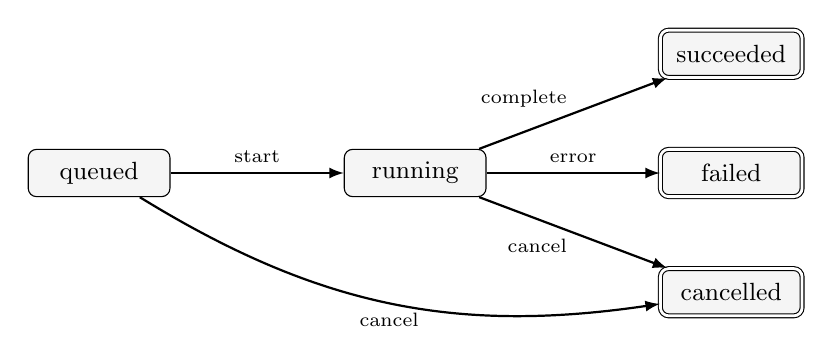
\begin{tikzpicture}[
    st/.style={rectangle, rounded corners=3pt, draw, fill=gray!8,
        minimum width=1.8cm, minimum height=0.6cm, font=\small},
    tm/.style={st, double, double distance=1pt},
    ar/.style={->, >=latex, thick},
    node distance=1.4cm and 2.2cm]
\node[st] (P) {queued};
\node[st, right=of P] (R) {running};
\node[tm, above right=0.9cm and 2.2cm of R] (S) {succeeded};
\node[tm, right=of R] (F) {failed};
\node[tm, below right=0.9cm and 2.2cm of R] (C) {cancelled};
\draw[ar] (P) -- node[above, font=\scriptsize] {start} (R);
\draw[ar] (R) -- node[above left=-2pt, font=\scriptsize] {complete} (S);
\draw[ar] (R) -- node[above, font=\scriptsize] {error} (F);
\draw[ar] (R) -- node[below left=-2pt, font=\scriptsize] {cancel} (C);
\draw[ar] (P) to[bend right=20] node[below, font=\scriptsize] {cancel} (C);
\end{tikzpicture}
\caption{Agent-run lifecycle state machine (FR-AE-01, EC-FC-01).
    Double-bordered states are terminal.}
\label{fig:run-sm}
\end{figure}

An agent run is created in the \emph{queued} state when the API
accepts a prompt.  Once the orchestrator begins execution the run
transitions to \emph{running}.  From \emph{running}, three terminal
transitions are possible: \emph{succeeded} on normal completion,
\emph{failed} on an unrecoverable error, or \emph{cancelled} when a
client-initiated cancellation request is honoured.  A run may also move
directly from \emph{queued} to \emph{cancelled} if the cancellation
arrives before the orchestrator picks up the request.

\begin{figure}[ht]
\centering
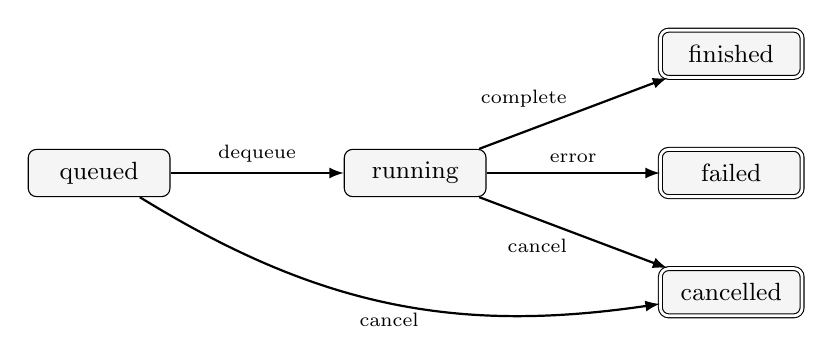
\begin{tikzpicture}[
    st/.style={rectangle, rounded corners=3pt, draw, fill=gray!8,
        minimum width=1.8cm, minimum height=0.6cm, font=\small},
    tm/.style={st, double, double distance=1pt},
    ar/.style={->, >=latex, thick},
    node distance=1.4cm and 2.2cm]
\node[st] (Q) {queued};
\node[st, right=of Q] (R) {running};
\node[tm, above right=0.9cm and 2.2cm of R] (Fi) {finished};
\node[tm, right=of R] (Fa) {failed};
\node[tm, below right=0.9cm and 2.2cm of R] (C) {cancelled};
\draw[ar] (Q) -- node[above, font=\scriptsize] {dequeue} (R);
\draw[ar] (R) -- node[above left=-2pt, font=\scriptsize] {complete} (Fi);
\draw[ar] (R) -- node[above, font=\scriptsize] {error} (Fa);
\draw[ar] (R) -- node[below left=-2pt, font=\scriptsize] {cancel} (C);
\draw[ar] (Q) to[bend right=20] node[below, font=\scriptsize] {cancel} (C);
\end{tikzpicture}
\caption{Job lifecycle state machine (FR-JB-02, EC-FC-07).
    Cancellation is cooperative: the worker checks a cancellation flag between steps.}
\label{fig:job-sm}
\end{figure}

A job enters the \emph{queued} state when it is persisted in the
control-plane database and its identifier is pushed onto the
appropriate queue in the in-memory store.  A dedicated worker process
dequeues the identifier, loads the metadata, and transitions the job to
\emph{running}.  Terminal states mirror those of an agent run:
\emph{finished} on success, \emph{failed} on error, or
\emph{cancelled} when the cooperative cancellation flag (stored in the
in-memory store and checked between orchestration steps) is detected.
Throughout the \emph{running} state the worker emits heartbeat updates;
if the heartbeat ceases, a supervisor can detect the orphaned job and
re-enqueue it (NFR-RE-06).


%----------------------------------------------------------------------
\section{Extended tables}
\label{app:extended-tables}
%----------------------------------------------------------------------

This section expands the traceability summary presented in
Table~\ref{tab:traceability} (Section~\ref{sec:requirements}) by
listing every core-tracked requirement group alongside its
implementation status and the evaluation criteria through which the
group is verified.  The platform defines 127 requirements: 73
functional (eight groups) and 54 non-functional (eight groups).  Of the
87~requirements classified as \emph{core tracked} (those mapped to
quantitative evaluation criteria), 80 are fully implemented and seven
are partially implemented; no requirement is left unaddressed.

\paragraph{Requirements coverage by category.}
Table~\ref{tab:app-req-coverage} summarises implementation status per
requirement group.  The remaining 40~requirements (from FR-AD, FR-UI,
NFR-AU, NFR-SC, NFR-RL, and two FR-JB items) are
implementation-support requirements verified through integration and
end-to-end tests rather than dedicated evaluation criteria.

\begin{table}[ht]
\centering
\caption{Requirements implementation coverage (core-tracked set;
    groups whose total exceeds this column have additional
    implementation-support items verified through integration tests).}
\label{tab:app-req-coverage}
\footnotesize
\begin{tabularx}{\textwidth}{@{}l c c c c X@{}}
    \hline
    \textbf{Group} & \textbf{Core} & \textbf{Full} & \textbf{Partial}
        & \textbf{None} & \textbf{Evaluation criteria} \\
    \hline
    FR-AE (Agent exec.)     & 10 & 10 & 0 & 0 & EC-FC-01\,.\,.\,04, EC-PF-02 \\
    FR-MM (Model mgmt.)     &  8 &  7 & 1 & 0 & EC-RE-01\,.\,.\,03 \\
    FR-TL (Tool ecosystem)  &  9 &  8 & 1 & 0 & EC-FC-06, EC-PF-04, EC-SE-02 \\
    FR-GQ (Graph query)     &  9 &  8 & 1 & 0 & EC-FC-05, EC-PF-03, EC-SE-03 \\
    FR-JB (Background jobs) &  9 &  9 & 0 & 0 & EC-FC-07\,.\,.\,08, EC-PF-05\,.\,.\,07 \\
    FR-AP (API design)      &  8 &  6 & 2 & 0 & (integration tests) \\
    NFR-SE (Security)       & 10 & 10 & 0 & 0 & EC-SE-01\,.\,.\,10 \\
    NFR-MT (Multi-tenancy)  &  8 &  7 & 1 & 0 & EC-SE-03 \\
    NFR-RE (Reliability)    &  8 &  7 & 1 & 0 & EC-RE-01\,.\,.\,08 \\
    NFR-OB (Observability)  &  8 &  8 & 0 & 0 & EC-OB-01\,.\,.\,08 \\
    \hline
    \textbf{Total (tracked)} & \textbf{87} & \textbf{80} & \textbf{7}
        & \textbf{0} & \\
    \hline
\end{tabularx}
\end{table}

\paragraph{Partially implemented requirements.}
Seven requirements are classified as partially implemented.  All seven
carry \emph{Should} or \emph{Could} priority in the MoSCoW
classification and therefore fall outside the minimum viability
threshold.  Table~\ref{tab:app-partial-reqs} identifies each and
summarises the gap.

\begin{table}[ht]
\centering
\caption{Partially implemented requirements and gap descriptions.}
\label{tab:app-partial-reqs}
\small
\begin{tabularx}{\textwidth}{@{}l l X@{}}
    \hline
    \textbf{ID} & \textbf{Priority} & \textbf{Gap description} \\
    \hline
    FR-MM-07 & Could & Model warmup reduces cold-start latency but
        is not invoked automatically on startup for all providers. \\
    FR-TL-07 & Should & Tool-level rate limiting exists but uses a
        shared counter rather than per-tool buckets. \\
    FR-GQ-08 & Could & Query caching is implemented for graph reads
        but TTL is not yet tenant-configurable. \\
    FR-AP-04 & Should & ETag generation is present for selected GET
        endpoints; full coverage is pending. \\
    FR-AP-07 & Should & Deprecation headers are emitted for
        versioned endpoints but migration-guidance payloads are not
        yet included. \\
    NFR-MT-05 & Should & Tenant quotas are tracked but enforcement
        beyond rate limits is not yet activated. \\
    NFR-RE-03 & Should & Redis unavailability degrades caching
        gracefully; a small subset of rate-limit code paths still
        raises exceptions rather than falling back to in-memory
        counters. \\
    \hline
\end{tabularx}
\end{table}

\paragraph{Functional-requirements priority distribution.}
Table~\ref{tab:app-fr-moscow} shows the MoSCoW distribution of the 73
functional requirements.  All 45~\emph{Must} requirements are fully
implemented; the seven partial implementations affect only
\emph{Should} or \emph{Could} items.

\begin{table}[ht]
\centering
\caption{Functional requirements by MoSCoW priority.}
\label{tab:app-fr-moscow}
\small
\begin{tabularx}{\textwidth}{@{}l c c c c@{}}
    \hline
    \textbf{Group} & \textbf{Must} & \textbf{Should} & \textbf{Could}
        & \textbf{Total} \\
    \hline
    Agent Execution (FR-AE)      & 7  & 3 & 0 & 10 \\
    Model Management (FR-MM)     & 4  & 3 & 1 &  8 \\
    Tool Ecosystem (FR-TL)       & 7  & 2 & 0 &  9 \\
    Graph Query (FR-GQ)          & 6  & 2 & 1 &  9 \\
    Background Jobs (FR-JB)      & 7  & 4 & 0 & 11 \\
    Administration (FR-AD)       & 5  & 4 & 1 & 10 \\
    API Design (FR-AP)           & 6  & 2 & 0 &  8 \\
    User Interface (FR-UI)       & 3  & 5 & 0 &  8 \\
    \hline
    \textbf{Total}               & \textbf{45} & \textbf{25} &
        \textbf{3} & \textbf{73} \\
    \hline
\end{tabularx}
\end{table}


%----------------------------------------------------------------------
\section{Reproducibility notes}
\label{app:reproducibility}
%----------------------------------------------------------------------

All quantitative results reported in Chapter~\ref{ch:results} were
produced from a single frozen snapshot of the platform at commit
\texttt{9b3e4c19} (2025-12-18).  Table~\ref{tab:app-env} documents the
software environment; the following paragraphs describe how to
replicate the evaluation.

\begin{table}[ht]
\centering
\caption{Evaluation environment.}
\label{tab:app-env}
\small
\begin{tabularx}{\textwidth}{@{}l X@{}}
    \hline
    \textbf{Component} & \textbf{Version / Configuration} \\
    \hline
    Hardware          & 2016 MacBook~Pro, Intel Core~i7-6820HQ 2.7\,GHz (4~cores / 8~threads), 16\,GB DDR3 \\
    Operating system  & macOS (Darwin kernel) \\
    Python runtime    & CPython 3.11.8 \\
    Web framework     & FastAPI 0.115.x with Uvicorn ASGI server \\
    Relational store  & PostgreSQL 16.x \\
    In-memory store   & Redis 7.x \\
    Graph database    & Memgraph 2.x (container image) \\
    Test framework    & pytest 8.4.x with pytest-asyncio \\
    Load tester       & Locust 2.x (single-machine mode) \\
    LLM providers     & OpenAI API (gpt-4o-mini), Ollama (local, llama3.2) \\
    \hline
\end{tabularx}
\end{table}

\paragraph{Environment setup.}
The evaluation requires three external services---a relational database,
an in-memory store, and a graph database---all of which can be started
via the project's container-orchestration configuration.  The
application itself runs outside the containers so that profiling tools
can attach directly to the Python process.  After installing the Python
dependencies declared in the project manifest, the API server is
launched with environment variables pointing to the three services and
to the OIDC provider used for authentication.

\paragraph{Running the test suite.}
The full test suite (3\,078~tests at the snapshot commit) is executed
through a single invocation of the test runner.  Tests are organised
into directories that mirror the evaluation structure:
\emph{security} tests (EC-SE), \emph{api} contract tests,
\emph{jobs} lifecycle tests, \emph{integration} tests for tool
invocation and graph query, and \emph{e2e} workflow tests.  Selective
execution is available by specifying individual directories or by using
category-based filters (e.g., selecting only performance or security
tests).

\paragraph{Load testing.}
Performance results (EC-PF-01 through EC-PF-07) were obtained using the
load-testing framework at five concurrency levels---1~user (sequential
baseline), 10, 50, 100, and 500~concurrent users---each preceded by a
thirty-second warm-up phase and measured during a sixty-second
steady-state window; every configuration was executed three times and
the median is reported (see Section~\ref{sec:repro-contract}).  The test
profiles exercise health probes, CRUD endpoints, tool invocations, and
job submissions.  Load-test scripts produce CSV files and HTML dashboards
that can be compared against the targets in Table~\ref{tab:ec-pf}.

\paragraph{Threat to reproducibility.}
Because agent-orchestration tests invoke live LLM providers, results may
vary if the provider's model weights are updated or if the service
experiences transient degradation.  The deterministic NL-to-Cypher test
mode (which replaces the LLM call with pre-recorded responses) mitigates
this for graph-query accuracy tests; however, end-to-end orchestration
latency and token-consumption figures remain provider-dependent.

\bigskip
\noindent
In summary, this appendix has provided the reference tables, formal
state-machine diagrams, extended traceability data, and reproduction
procedure that support the claims made in the main body of the thesis.
Together, these materials enable an independent reader to verify the
tool and endpoint counts cited in the evaluation (EQ1), trace every
requirement to its evaluation outcome (EQ1--EQ4), inspect the lifecycle
invariants enforced by the platform, and reproduce the quantitative
results under equivalent conditions.

%%%%%%%%%%%%%%%%%%%%%%%%%%%%%%%%%%%%%%%%%%%%%%%%%%%%%%%%%%%%%%%%%%%%%%%%%%%%%%%
%% BIBLIOGRAPHY
%%%%%%%%%%%%%%%%%%%%%%%%%%%%%%%%%%%%%%%%%%%%%%%%%%%%%%%%%%%%%%%%%%%%%%%%%%%%%%%

\backmatter

\bibliographystyle{sapthesis}
\bibliography{references}

\end{document}
